\documentclass[12pt]{article}

% ============================================================================
% PREAMBLE - Package Imports and Setup
% ============================================================================

% --- Page Layout ---
\usepackage[margin=1in]{geometry}
\usepackage{setspace}
\doublespacing

% --- Fonts ---
% mathptmx and times require rsfs/pcr fonts not in TeX Live 2025 basic.
% Using default Computer Modern for now; switch to mathptmx when full TeX Live is available.
%\usepackage{mathptmx}  % Times Roman font (needs rsfs package)
\usepackage[T1]{fontenc}

% --- Mathematics ---
\usepackage{amsmath,amssymb,amsthm}
\usepackage{mathtools}
\usepackage{bm}  % Bold math symbols

% --- Graphics and Figures ---
\usepackage{graphicx}
\usepackage{subcaption}
\usepackage{tikz}
% \usepackage{pgfplots}  % Not used in current version
% \pgfplotsset{compat=1.18}
\usetikzlibrary{arrows,shapes,positioning,calc,decorations.pathreplacing}

% --- Tables ---
\usepackage{booktabs}
% \usepackage{multirow}  % Not used in current version
\usepackage{array}

% --- Algorithms ---
% Using custom algorithm environment (no algorithm2e dependency)
\usepackage{ifthen}
\newcounter{algorithm}
\renewcommand{\thealgorithm}{\arabic{algorithm}}
\newenvironment{algorithmbox}[1][]{%
  \refstepcounter{algorithm}%
  \begin{center}\begin{minipage}{0.92\textwidth}%
  \rule{\textwidth}{0.4pt}\par\smallskip%
  \textbf{Algorithm \thealgorithm}\ifthenelse{\equal{#1}{}}{}{: #1}\par\smallskip%
  \rule{\textwidth}{0.4pt}\par\smallskip%
}{%
  \par\smallskip\rule{\textwidth}{0.4pt}%
  \end{minipage}\end{center}%
}

% --- Bibliography ---
\usepackage[authoryear,round]{natbib}
\bibliographystyle{plainnat}

% --- Hyperlinks and Cross-References ---
\usepackage{hyperref}
\hypersetup{
    colorlinks=true,
    linkcolor=blue,
    citecolor=blue,
    urlcolor=blue,
    pdfauthor={Mátyás Farkas},
    pdftitle={Investment Adjustment Costs and Nonlinear Solution Gaps in Smets--Wouters}
}
% \usepackage[capitalize]{cleveref}  % Replaced with standard \ref

% --- Other Utilities ---
\usepackage{enumitem}
\usepackage{xcolor}

% --- Submission/Archive Switch ---
% Default compile is the short submission paper. Define \WITHPAPERAPPENDIX
% before inputting this file to compile the legacy in-file appendices.
\newif\ifpaperappendix
\paperappendixfalse
\ifdefined\WITHPAPERAPPENDIX
  \paperappendixtrue
\fi
\newcommand{\paperappref}[1]{\ifpaperappendix Appendix~\ref{#1}\else online appendix\fi}
\newcommand{\paperapprefs}[2]{\ifpaperappendix Appendices~\ref{#1} and~\ref{#2}\else online technical appendix\fi}
\newcommand{\paperappnote}[2]{\ifpaperappendix Appendix~\ref{#1}#2\else online appendix\fi}

% ============================================================================
% THEOREM ENVIRONMENTS
% ============================================================================

\theoremstyle{plain}
\newtheorem{theorem}{Theorem}[section]
\newtheorem{proposition}[theorem]{Proposition}
\newtheorem{lemma}[theorem]{Lemma}
\newtheorem{corollary}[theorem]{Corollary}

\theoremstyle{definition}
\newtheorem{definition}[theorem]{Definition}
\newtheorem{assumption}[theorem]{Assumption}
\newtheorem{example}[theorem]{Example}

\theoremstyle{remark}
\newtheorem{remark}[theorem]{Remark}

% ============================================================================
% CUSTOM COMMANDS
% ============================================================================

% --- Mathematical Operators ---
\DeclareMathOperator{\E}{\mathbb{E}}
\DeclareMathOperator{\Var}{\text{Var}}
\DeclareMathOperator{\Cov}{\text{Cov}}
\DeclareMathOperator{\argmin}{argmin}
\DeclareMathOperator{\argmax}{argmax}
\DeclareMathOperator{\tr}{tr}
\DeclareMathOperator{\diag}{diag}

% --- Custom Math Symbols ---
\newcommand{\R}{\mathbb{R}}
\newcommand{\N}{\mathbb{N}}
\newcommand{\given}{\,|\,}
\newcommand{\ind}{\mathbb{1}}

% --- Table Notes ---
\newcommand{\tablenotes}[1]{%
  \par\vspace{0.5em}%
  \noindent\begin{minipage}{\textwidth}%
  \raggedright\footnotesize #1%
  \end{minipage}\par%
}

% --- Model Notation ---
\newcommand{\eps}{\varepsilon}
\newcommand{\Sigmay}{\Sigma_y}
\newcommand{\Sigmaeps}{\Sigma_\varepsilon}

% ============================================================================
% TITLE PAGE
% ============================================================================
\vspace{-3cm}
\small \title{\textbf{Investment Adjustment Costs and Nonlinear Solution Gaps in Smets--Wouters}\thanks{I am grateful to Fabio Canova, Kai Christoffel, Chris Erceg, Jesper Lind\'e, Zolt\'an Jakab, Thore Klockerols, and Marcin Kolasa for insightful discussions and comments.  All errors are my own. The views expressed herein are those of the author and not necessarily those of the International Monetary Fund.}}
\small \author{Mátyás Farkas\thanks{mfarkas@imf.org}\\
\footnotesize International Monetary Fund}
\vspace{-1cm}
\footnotesize \date{\today\\
\footnotesize \textit{Preliminary --- Comments Welcome}}

% ============================================================================
% DOCUMENT BEGIN
% ============================================================================

\begin{document}

\begingroup
\singlespacing
\maketitle
\vspace{-1cm}
\begin{abstract}
\noindent
\footnotesize
This paper asks what the first-order approximation to Smets--Wouters misses. In the
Holden--Lind\'e--Trabandt (HLT) specification and audited support studied here,
the largest measured gap is not mainly the effective lower bound or Kimball
pricing. It is the investment block. A stochastic-extended-path decomposition
assigns 69 percent of the nonlinear-minus-linear solution gap to investment and
capital, and 0.2 percent to the price Phillips curve. The core mechanism is simple:
the level investment adjustment cost has zero value and zero marginal cost at
trend growth, while first order compresses the state-dependent marginal-cost
products into local coefficients.

I take the nonlinear model to U.S. data with a neural network that learns only
the residual between the nonlinear and first-order transitions. A gate applies
this correction when the economy is far from steady state. In a reduced
four-parameter HLT bridge, all 10{,}000 supported direct-SEP cells converge; the
surrogate lowers prediction RMSE from 0.1436 to 0.00075 and grid log-criterion
surface RMSE from 88.07 to 0.053. The empirical HMC results are conditional and
criterion-based, not marginal-likelihood comparisons. In the 1959--2025 sample,
a high-objective warm-started surrogate mode improves the chain-mean
profiled hybrid criterion by 35.92 nats relative to the linear Kalman posterior
mean, and the linear smoother requires risk-premium shocks of $56\sigma$ during
COVID. But restoring the ARMA(1,1) markup terms improves the linear likelihood
by 34 nats on the baseline sample, nearly matching the extended-sample
surrogate criterion gap, and calm-period forecasting remains gate-sensitive.
The result is evidence for an important investment-channel nonlinearity in this
HLT benchmark, not a specification-invariant rejection of linear DSGE
estimation.
\end{abstract}

\medskip
\noindent \textbf{JEL Classification:} C11, C13, C32, C63, E47

\noindent \textbf{Keywords:} DSGE models, nonlinear estimation, investment adjustment costs, perturbation bias, neural network surrogates, occasionally binding constraints
\endgroup

\clearpage

\tableofcontents
\clearpage

% ============================================================================
% SECTION 1: INTRODUCTION
% ============================================================================

\section{Introduction}
\label{sec:introduction}

Nonlinear DSGE estimation is usually motivated by the effective lower bound
(ELB). The ELB matters, and a large literature has built nonlinear tools to
handle it \citep{gust2012effects,boehl2022monetary,guerrieri2015occbin}. This
paper asks a different question: in the Smets--Wouters model as implemented by
Holden--Lind\'e--Trabandt (HLT), where is the largest nonlinear error from
using the first-order approximation?

The answer is the investment block. I solve the nonlinear model by stochastic
extended path (SEP) at 22,080 state--shock--parameter points and compare each
solution with the first-order solution. Investment and capital account for 69
percent of the nonlinear-minus-linear gap. The price Phillips curve accounts
for 0.2 percent. When lower-bound episodes are added, investment remains the
largest unconditional source of the gap (Figure~\ref{fig:decomposition_vs_scale}).

The mechanism is transparent. With \(x_t=I_t/I_{t-1}\), the level adjustment
cost is locally \(S(x_t)=\tfrac{\chi}{2}(x_t-1)^2\). At trend growth,
\(S(1)=S_x(1)=0\). The level resource cost is therefore invisible to first
order. The marginal term \(S_x(x_t)\) is locally visible, but first order keeps
only a local coefficient and drops products involving \(S_x\), Tobin's \(q\),
the shadow price of capital, and the stochastic discount factor. A Gal\'i
negative-control model with a lower bound but no investment block has small
gaps at relevant shock scales (Figure~\ref{fig:gali_obc_vs_no_obc}).

To estimate the nonlinear model, I denote the first-order perturbation solution
by ROM1 and use a surrogate that learns only what ROM1 misses:
\[
  \Delta g_\theta = g_\theta^{\mathrm{SEP}}-g_\theta^{\mathrm{ROM1}}.
\]
The estimator adds the learned residual to the linear solution only when the
state is far from steady state. This keeps the computation feasible and gives a
direct validation target. In a reduced four-parameter HLT bridge, all
10{,}000 supported direct-SEP cells converge; the surrogate lowers prediction RMSE
from 0.1436 to 0.00075 and grid log-criterion surface RMSE from 88.07 to 0.053. The
online technical appendix documents the computation, output files, and
validation criteria.

The empirical HMC results are useful but conditional. In the 1959--2004 sample,
regime-switching surrogate estimation under the profiled criterion is associated
with higher risk-premium volatility and lower wage-markup persistence. In the
1959--2025 sample, a high-objective warm-started surrogate mode improves the
posterior-mean profiled hybrid criterion by 35.92 nats, and the linear smoother
requires risk-premium shocks of \(56\sigma\) during COVID. This comparison is
not a Bayes factor. It is conditional on one U.S. sample, one HLT
specification, one explored posterior basin, the surrogate approximation, the
profiled inversion objective, the gate, and COVID out-of-distribution risk.

One specification issue is central. The HLT baseline suppresses the ARMA(1,1)
price- and wage-markup shock terms used by \citet{smets2007shocks}. This is the
same block where \citet{farkas2020bayesian} document a flat posterior target.
Restoring those MA terms improves the linear log likelihood by 34 nats on the
baseline sample, almost the same size as the surrogate criterion gap in the
extended sample. This materially limits the empirical interpretation: the
parameter shifts are evidence relative to the restricted HLT benchmark, not a
specification-invariant rejection of linear DSGE estimation or a clean
nonlinear-investment effect absent restored markup dynamics.

The main message is narrow. For SW-style models with level investment
adjustment costs, this evidence makes the investment block a priority
diagnostic. The deterministic decomposition is the strongest evidence. The
criterion-based parameter comparison supports the same mechanism, but it
remains model- and implementation-specific. Calm-period forecasting confirms
the caution: the original gate fails on 1995Q1--2007Q4, and a q95 padded
re-estimation improves the aggregate RMSE ratio to 1.09 but does not beat ROM1
over the full quiet holdout.

The paper connects three literatures: nonlinear solution of DSGE models by SEP
\citep{fair1983solution,adjemian2025stochastic}, surrogate methods for
expensive models \citep{peherstorfer2018survey,kennedy2001bayesian,kase2025estimating,naubert2025differentiable},
and filter-free HMC estimation of DSGE models
\citep{childers2022filter,farkas2020bayesian}. The contribution here is to use
the surrogate as an auditable bridge between a direct nonlinear solution and a
criterion-based empirical HMC comparison.

% ============================================================================
% SECTION 3: THE INVISIBILITY PROPERTY
% ============================================================================

\section{The Invisibility Property}
\label{sec:invisibility}

Before computing anything, I characterize analytically which nonlinearities in a DSGE model are visible to first-order perturbation and which are not.

\subsection{A General Perturbation Invisibility Result}

\begin{proposition}[Perturbation Invisibility]
\label{prop:invisibility}
Let $f: \mathbb{R} \to \mathbb{R}$ enter an equilibrium condition of a DSGE model evaluated at a variable $x_t$ with steady-state value $\bar{x}$. If $f(\bar{x}) = 0$ and $f'(\bar{x}) = 0$, then $f$ contributes zero to the first-order perturbation solution. Specifically, defining $\hat{x}_t = x_t - \bar{x}$, the Taylor expansion $f(x_t) = f(\bar{x}) + f'(\bar{x})\hat{x}_t + \tfrac{1}{2}f''(\bar{x})\hat{x}_t^2 + \mathcal{O}(\hat{x}_t^3)$ reduces to $f(x_t) = \tfrac{1}{2}f''(\bar{x})\hat{x}_t^2 + \mathcal{O}(\hat{x}_t^3)$, which is identically zero at first order.
\end{proposition}

The proof is immediate from the definition of first-order perturbation, which retains only terms linear in $\hat{x}_t$. Three observations sharpen the economic content.

First, the investment adjustment cost can be written locally as $S(x) = \tfrac{\chi}{2}(x-1)^2$ for $x = I_t/I_{t-1}$, with $\chi=S_{xx}(1)$. This level cost satisfies both conditions at the balanced-growth point $x=1$: $S(1) = 0$ because the cost vanishes when investment grows at trend, and $S_x(1) = 0$ because the cost function is designed to have zero marginal cost at trend. At the \citet{smets2007shocks} calibration $\chi \approx 6.06$ in the normalization used here. Every basis point of the level resource cost that the full nonlinear solver evaluates is therefore a pure second-order object that linearization discards. The marginal cost $S_x(x)=\chi(x-1)$ is locally first order, so the formal claim is narrower: the level cost is invisible, while the nonlinear residual in the investment first-order condition arises from products and future terms involving $S_x$.

Second, the capital utilization cost $a(z) = \tfrac{r^k_{ss}}{c_z}[\exp(c_z(z-1)) - 1]$ does \emph{not} satisfy the invisibility condition: $a(1) = 0$ but $a'(1) = r^k_{ss} \neq 0$. The first-order utilization response is therefore captured by perturbation; only the curvature of $a(\cdot)$ is lost, and that curvature ($a''(1) \approx 0.005$) is roughly 1,200 times smaller than $S''(1)$. More generally, any function with $f'(\bar{x}) \neq 0$ has its dominant effect captured by linearization, with only the residual curvature lost.

Third, the Kimball price and wage aggregators exhibit high formal curvature (power-law exponents of $\pm 7$), but price and wage dispersion indices remain within $10^{-4}$ of unity under Calvo pricing. The effective curvature---formal curvature times the squared deviation from steady state---is therefore negligible. High mathematical curvature alone is not sufficient; the variable must also move far enough from steady state for that curvature to matter.

\subsection{Analytical Ranking of Nonlinearity Sources}

The HLT implementation contains seven sources of nonlinearity. I rank them by the quadratic-to-linear (Q/L) ratio: the second-order Taylor term divided by the first-order term, evaluated at one standard deviation of the relevant variable. A higher ratio means a larger share of the function's effect comes from curvature that linearization discards.

The investment first-order condition dominates: Q/L = 18.7\% at $1\sigma$. The local slope of $S_x$ is present in the first-order condition, but products involving $S_x$, capital prices, and stochastic discount factors generate second-order terms that are sizable at empirically relevant state displacements. Linearization captures the local marginal slope and misses these state-dependent interaction terms.

The Kimball wage first-order condition ranks second at Q/L = 2.8\%. Wages are stickier than prices ($\xi_w = 0.81$ vs.\ $\xi_p = 0.60$), producing cross-sectional wage dispersion an order of magnitude larger than price dispersion, so the $\tilde{w}^{-6}$ power generates meaningful curvature. Habit-amplified marginal utility is close behind at Q/L = 2.7\%: the habit-adjusted consumption base is only 36.6 percent of steady-state consumption, amplifying the curvature of $(C_t - hC_{t-1}/\gamma)^{-\sigma}$ roughly $7.5\times$. The remaining sources---non-separable marginal utility (1.2\%), Kimball wage dispersion (0.8\%), and Kimball price dispersion (below 0.1 percent)---are progressively smaller. The ELB contributes only above $3\sigma$ (Figure~\ref{fig:gali_obc_vs_no_obc}); at empirically relevant scales it is a kink that piecewise-linear methods handle well \citep{guerrieri2015occbin}.

The ranking predicts that the investment block should dominate the
SEP--ROM1 gap, the wage block should contribute modestly, and the pricing block
and ELB should be small at empirically relevant shock scales.
Section~\ref{sec:decomposition} finds patterns consistent with these
predictions.


% ============================================================================
% SECTION 4: MODEL ENVIRONMENT
% ============================================================================

\section{Model Environment}
\label{sec:model}

\subsection{General DSGE Framework}

The notation is standard. The nonlinear model is a system of equilibrium
conditions,
\begin{equation}
\label{eq:equilibrium}
\E_t\left[F(s_{t+1}, s_t, s_{t-1}, \eps_t; \theta)\right] = 0,
\end{equation}
where \(s_t\) collects states and jumps, \(\eps_t\) are standardized shocks,
and \(\theta\) are structural parameters. A solution is a transition rule
\begin{equation*}
s_t = g_\theta(s_{t-1}, \eps_t),
\end{equation*}
that satisfies \eqref{eq:equilibrium}. The paper compares two transition
rules: the first-order perturbation \(g_\theta^{\mathrm{ROM1}}\), which I call
ROM1, and the direct nonlinear stochastic-extended-path solution
\(g_\theta^{\mathrm{SEP}}\). I use full-order model (FOM) as shorthand for this
direct SEP benchmark.

\subsection{Observation Equation}

Observed data are
\begin{equation}
\label{eq:observation}
y_t = H(s_t) + \eta_t, \quad \eta_t \sim \mathcal{N}(0, \Sigmay),
\end{equation}
with a linear measurement map \(H\). In the Gal\'i validation model, the
observables are output, inflation, and the nominal rate. In the
Smets--Wouters application, they are output growth, consumption growth,
investment growth, hours, inflation, wage growth, and the interest rate.

\subsection{Estimation Problem}

The object of interest is
\begin{equation}
\label{eq:posterior}
p(\theta \given y_{1:T}^{\text{obs}}) \propto p(y_{1:T}^{\text{obs}} \given \theta) \, p(\theta),
\end{equation}
with the linear Kalman likelihood as the benchmark. The nonlinear estimator
does not use a particle filter. It treats shocks as latent objects and either
samples them directly in small validation models or recovers them through an
inversion filter in the 18-parameter application. The full latent-shock density
would be
\begin{equation*}
\mathcal{L}(\theta, s_0, \eps_{1:T} \given y_{1:T}^{\text{obs}}) = \prod_{t=1}^T p(y_t^{\text{obs}} \given s_t; \Sigmay) \cdot p(s_0) \cdot \prod_{t=1}^T p(\eps_t),
\end{equation*}
where \(s_t=\hat g_\theta(s_{t-1},\eps_t)\). The empirical 18-parameter
surrogate runs use a profiled hybrid observation criterion rather than this
exact marginal likelihood: the recovered shocks are not integrated out, and the
shock-prior and determinant/Laplace terms needed for a likelihood comparison
are not included. This avoids the particle-weight degeneracy documented below
and keeps the empirical comparison operational in a medium-scale model.

\subsection{Illustrative Models}
\label{subsec:gali_model}

The Gal\'i (2015) model is a negative-control comparison. It has Calvo pricing,
a Taylor rule, and an occasionally binding lower bound, but no investment or
capital block:
\[
R_t = \max\{1, (R_{ss})^{1-\rho_R}(\Pi_t/\Pi_{ss})^{(1-\rho_R)\phi_\pi}(Y_t/Y_{ss})^{(1-\rho_R)\phi_y}R_{t-1}^{\rho_R}e^{\varepsilon_t^R}\},
\]
The online technical appendix reports the maintained ELB/OBC validation
package for this model.

The main application uses the HLT Smets--Wouters model: habit formation, capital
accumulation, investment adjustment costs, variable utilization, Kimball
demand, and the lower bound. I estimate 18 parameters: seven shock
persistences, seven shock volatilities, and four price/wage parameters
\((\xi_p,\iota_p,\varepsilon_p,\xi_w)\). The online technical appendix
summarizes the maintained computational pipeline and validation record.


% ============================================================================
% SECTION 5: NONLINEAR SOLUTION AND SURROGATE
% ============================================================================

\section{Nonlinear Solution and Surrogate}
\label{sec:methodology}

\subsection{Multi-Fidelity Architecture}
\label{subsec:multifidelity}

The estimator has one organizing principle: learn only the nonlinear part that
first order misses. I write
\[
  \Delta g_\theta(s,\eps)
  =
  g_\theta^{\mathrm{SEP}}(s,\eps)
  -
  g_\theta^{\mathrm{ROM1}}(s,\eps),
\qquad
  \hat g_\theta
  =
  g_\theta^{\mathrm{ROM1}}+\widehat{\Delta g}_\theta .
\]
The network targets \(\Delta g_\theta\), not \(g_\theta^{\mathrm{SEP}}\). This
keeps the target small and makes validation direct: on held-out SEP solves, the
error is exactly the error in the nonlinear correction.

The procedure is split in two. Offline, I draw parameter points, solve the
nonlinear model, compute the first-order solution at the same inputs, and train
the residual network. Online, I recover shocks through the inversion filter,
apply the residual only in stressed periods, and sample parameters with
NUTS-HMC. Since the inversion step profiles over shocks without the shock-prior
and determinant/Laplace terms needed for a likelihood, I call the resulting
object a profiled hybrid objective rather than a marginal likelihood.

\subsection{Stochastic Extended Path (SEP) Algorithm}
\label{subsec:sep}

SEP solves \eqref{eq:equilibrium} directly after approximating expectations by
Gauss--Hermite quadrature \citep{fair1983solution,adjemian2025stochastic}. The
unknowns are all future states on a finite shock tree. Stacking the equations
gives \(R(Y;\theta)=0\), solved by damped Newton steps,
\begin{equation}
\label{eq:newton_iteration}
Y^{(j+1)} = Y^{(j)} - \alpha^{(j)} \left[\frac{\partial R}{\partial Y}(Y^{(j)}; \theta)\right]^{-1} R(Y^{(j)}; \theta),
\end{equation}
where \(\alpha^{(j)}\) is chosen by line search. A single HLT SEP solve takes
about 0.8 seconds, which is too slow to put inside every HMC leapfrog step but
fast enough to generate an offline training set.

The lower bound is imposed inside the nonlinear system. For differentiability I
use a smooth softplus version,
\begin{equation}
R_t = 1 + \frac{1}{\kappa_s}\log\!\bigl(1 + e^{\kappa_s(\tilde{R}_t - 1)}\bigr), \label{eq:softplus_zlb}
\end{equation}
where \(\tilde R_t\) is the shadow Taylor-rule rate and \(\kappa_s=100\).
Details on quadrature, warm starts, and solver tolerances are in
the online technical appendix.


\subsection{Dataset Generation and Surrogate Training}
\label{subsec:surrogate}

Training is supervised learning. I choose Sobol parameter draws, simulate state
and shock inputs, solve SEP and ROM1 at the same inputs, and store
\begin{equation*}
\Delta y_j = g_\theta^{\text{SEP}}(x_j) - g_\theta^{\text{ROM1}}(x_j).
\end{equation*}
The 18-parameter dataset contains 22,080 usable samples. Held-out non-binding
RRMSE is about 0.0012. The lower-bound stress region is less accurate and is
treated separately. Architecture and training details are in
the online technical appendix.

\subsection{Regime-Switching Gate and Inversion Filter}
\label{subsec:regime_switching}

Not every period needs the nonlinear correction. I classify a period as
stressed when the state is far from steady state. Calm periods use ROM1;
stressed periods use the residual-corrected transition,
\begin{equation*}
s_t = (1-g_t)\,g_\theta^{\text{ROM1}}(s_{t-1}, \eps_t) + g_t\,\hat{g}_\theta(s_{t-1}, \eps_t).
\end{equation*}
The shocks are recovered period by period by an inversion filter. This keeps
the 18-parameter sampler low-dimensional. The price is that the stressed-period
criterion is a profiled Gaussian observation objective, not an exact likelihood;
recovering a likelihood would require the omitted shock-prior and
determinant/Laplace terms (online technical appendix).

\subsection{Filter-Free Hamiltonian Monte Carlo}
\label{subsec:hmc}

I sample with NUTS-HMC \citep{hoffman2014nuts}. In small validation models,
shocks and the initial state can be sampled jointly with \(\theta\). In the
18-parameter application, the inversion filter recovers shocks and NUTS samples
\(\theta\) alone. The linear baseline completes in 100 minutes; the
regime-switching surrogate completes in 2.4 hours. Both baseline runs have zero
divergent transitions. Details are in the online technical appendix.


% Identification and Validation details are in Appendices~\ref{sec:identification} and~\ref{sec:validation_design}.

With the estimation machinery in place, I turn to the central question: which nonlinearities in the Smets--Wouters model drive the gap between full-order and linear solutions?

\section{Quantitative Decomposition}
\label{sec:decomposition}

\subsection{The 69 Percent Finding}
\label{subsec:nonlinearity_sources}

Each training sample records both the full-order (SEP) and first-order perturbation (ROM1) transitions at the same $(s_{t-1}, \varepsilon_t, \theta)$. Their difference isolates the nonlinear correction the surrogate must learn. I define the scalar nonlinearity measure as
\begin{equation*}
\Delta_j = \| g_\theta^{\text{FOM}}(s_{j}, \varepsilon_j) - g_\theta^{\text{ROM1}}(s_{j}, \varepsilon_j) \|_2,
\end{equation*}
where $g^{\text{FOM}}$ is the SEP solution and $g^{\text{ROM1}}$ is first-order perturbation. The decomposition draws on 22,080 training samples varying all 18 parameters. Figure~\ref{fig:nonlinearity_decomposition} summarizes: state distance dominates ($R^2 = 0.96$), parameters contribute modestly (11\%), and current-period shocks are negligible ($<0.3$\%).

\begin{figure}[t]
\centering
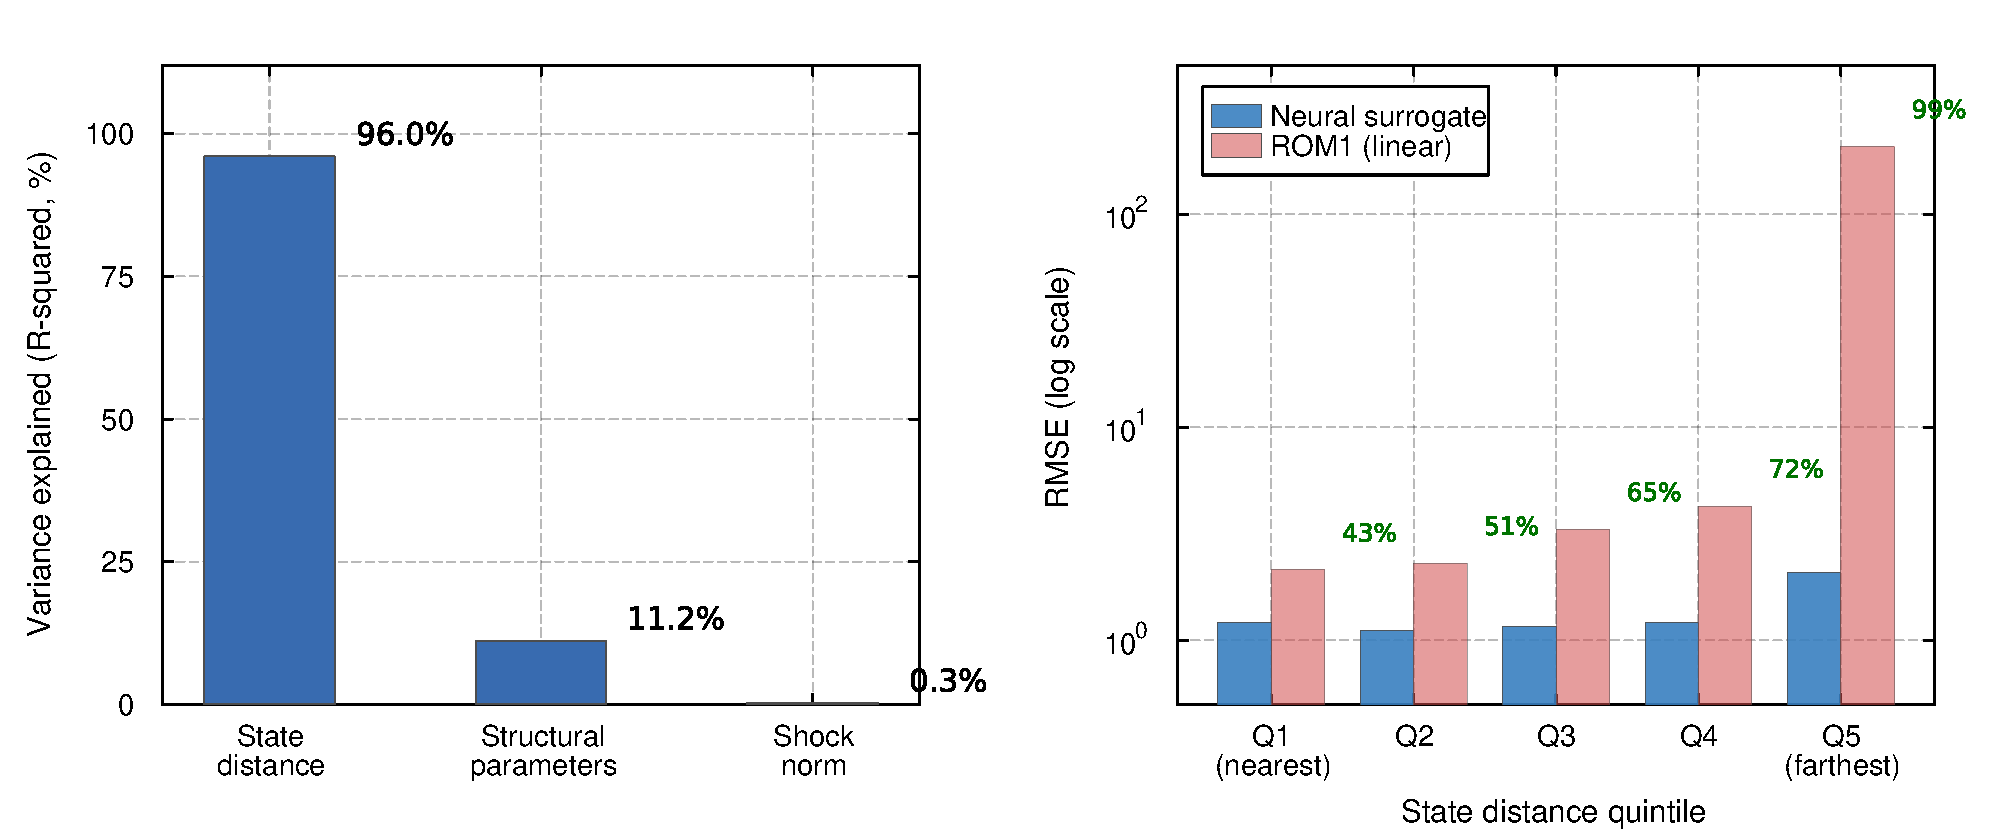
\includegraphics[width=\textwidth]{figures/fig_nonlinearity_combined.pdf}
\caption{Nonlinearity variance decomposition and surrogate accuracy by distance from steady state. Panel~(a): $R^2$ from regressing the nonlinearity measure $\Delta_j = \|g^{\text{FOM}} - g^{\text{ROM1}}\|_2$ on each feature set separately. Panel~(b): RMSE of the neural surrogate (blue) and first-order perturbation ROM1 (red) across quintiles of state distance $\|s - \bar{s}(\theta)\|_2$, with percentage improvement labeled. The surrogate's RMSE is roughly flat while ROM1 errors grow by two orders of magnitude. Based on 22,080 training samples from the 18-parameter dataset.}
\label{fig:nonlinearity_decomposition}
\end{figure}

On the maintained training support, state distance has the highest predictive power for the nonlinear correction ($R^2 = 0.960$). ROM1 errors grow by two orders of magnitude from the nearest to the farthest state-distance quintile; the surrogate stays flat, achieving 99 percent improvement in the farthest quintile in the maintained validation diagnostic.

The investment and capital block accounts for 69 percent of the total gap (Table~\ref{tab:equation_block}). The price Phillips curve---the block through which the Kimball aggregator enters and a common focus in nonlinear DSGE applications---contributes 0.2 percent.

\begin{table}[htbp]
\centering
\caption{Equation-Block Decomposition of the FOM--ROM1 Gap}
\label{tab:equation_block}
\begin{tabular}{lccc}
\toprule
Economic Block & Variables & Mean $\|\Delta\|_2$ & Share (\%) \\
\midrule
Investment / Capital & $\Delta i$, $k$, $q$, $z$, $r^k$, $a(z)$, $S'$, $q^s$ & 20.53 & 68.9 \\
Euler / Consumption & $\xi$, $c$, $\Delta c$ & 9.59 & 13.5 \\
Wage Phillips Curve & $w$, $\Delta w$, $\dot{w}$, $\gamma^w_{1{-}3}$, $s^w$ & 19.41 & 10.8 \\
Output / Production & $y$, $\Delta y$, hours, $S^D$ & 5.10 & 4.3 \\
Flex-Price Block & $c^f$, $y^f$, $i^f$, $k^f$, $q^f$, $r^{k,f}$ & 3.30 & 2.3 \\
Price Phillips Curve & $\pi$, $D_p$, $\dot{p}$, $\gamma_{1{-}3}$, $s^\pi$ & 1.85 & 0.2 \\
Monetary Policy & $r$, $r^{\text{obs}}$, $m$ & 0.61 & 0.1 \\
\bottomrule
\end{tabular}
\tablenotes{\textit{Notes}: Based on 22,080 training samples from the 18-parameter dataset, varying all 18 parameters across Sobol-drawn prior support. Mean $\|\Delta\|_2$ is the average Euclidean norm of the FOM--ROM1 gap for variables in each block. Share is the fraction of total $\sum_j \|\Delta_j\|_2^2$ attributable to each block. The ``FOM--ROM1 gap'' measures the difference between the nonlinear SEP solution and the first-order perturbation output at identical state--shock--parameter inputs. Shares may not sum to 100 due to rounding.}
\end{table}

Table~\ref{tab:equation_block} delivers the central result: the investment and capital block accounts for 68.9 percent of the total gap, while the price Phillips curve contributes just 0.2 percent. The mechanism involves three interacting nonlinear functions in the investment block: the exponential capital utilization cost $a(z_t)$, the quadratic investment adjustment cost $S(I_t/I_{t-1})$, and Tobin's $q$ dynamics. When a negative investment-specific shock depresses the shadow price of capital $p^k$, the adjustment cost for future recovery rises---a compounding $S_x \times p^k \times \xi_{t+1}/\xi_t$ interaction that linearization replaces with a constant coefficient. The Gal\'i (2015) model, which lacks investment entirely, shows small gaps even at $5\sigma$, consistent with this channel being the dominant source in this decomposition.

The adjustment cost $S'$ itself contributes only 2 percent of the state-level gap, but its nonlinearity propagates through Tobin's $q$ into the stochastic discount factor $\xi_t$, which enters every forward-looking equation. The investment channel generates the nonlinear impulse; the discount factor transmits it economy-wide.

Structural parameters explain 11 percent of nonlinearity variation in separate diagnostic regressions. The strongest correlates are government spending persistence $\rho_g$ ($+0.18$), risk-premium volatility $\sigma_b$ ($+0.17$), and Kimball curvature $\varepsilon_p$ ($-0.11$)---higher curvature flattens demand and makes the model \emph{more} linear. Current-period shocks contribute negligibly ($R^2 = 0.0003$). Nonlinearity accumulates through persistent displacement, clustering in temporal bursts with autocorrelation 0.81 and mean duration 12.5 quarters; per-observable diagnostic $R^2$ values remain below 12 percent.

These patterns suggest possible parameter shifts, but the sign can depend on
the sample period, objective, gate, and posterior basin. In the baseline
1959--2004 regime-switching surrogate run, the 18-parameter results
(Section~\ref{par:results_18param_switching}) line up with three such margins:
$\sigma_b$ doubles, $\rho_w$ falls 80 percent, and $\varepsilon_p$ rises
2.7-fold.


\subsection{State-Dependent Impulse Responses}
\label{subsec:irf_comparison}

Under ROM1, impulse responses scale linearly and are symmetric in the sign of the shock. Under SEP, neither property holds. For investment-specific shocks at magnitudes from $1\sigma$ to $5\sigma$, the solutions coincide at small shocks but diverge substantially by $5\sigma$. Positive shocks are amplified, consistent with the quadratic adjustment cost $S$ compounding with the consumption-savings wedge; negative shocks are asymmetrically attenuated, consistent with the convex utilization cost $a(z)$ damping downward adjustment. The risk premium shock shows the same pattern through the Tobin's $q$ channel; the price markup shock shows minimal divergence in the maintained impulse-response diagnostic.

The seven-observable response to a $4\sigma$ investment shock supports the equation-block decomposition (Figure~\ref{fig:all_vars_eqs}): nonlinear amplification concentrates in investment growth, spills to output and hours, and leaves inflation and the interest rate nearly unchanged. The correction surface peaks in the first 5--10 quarters and grows nonlinearly with shock size---the $5\sigma$ correction is not five times the $1\sigma$ correction.

\begin{figure}[t]
\centering
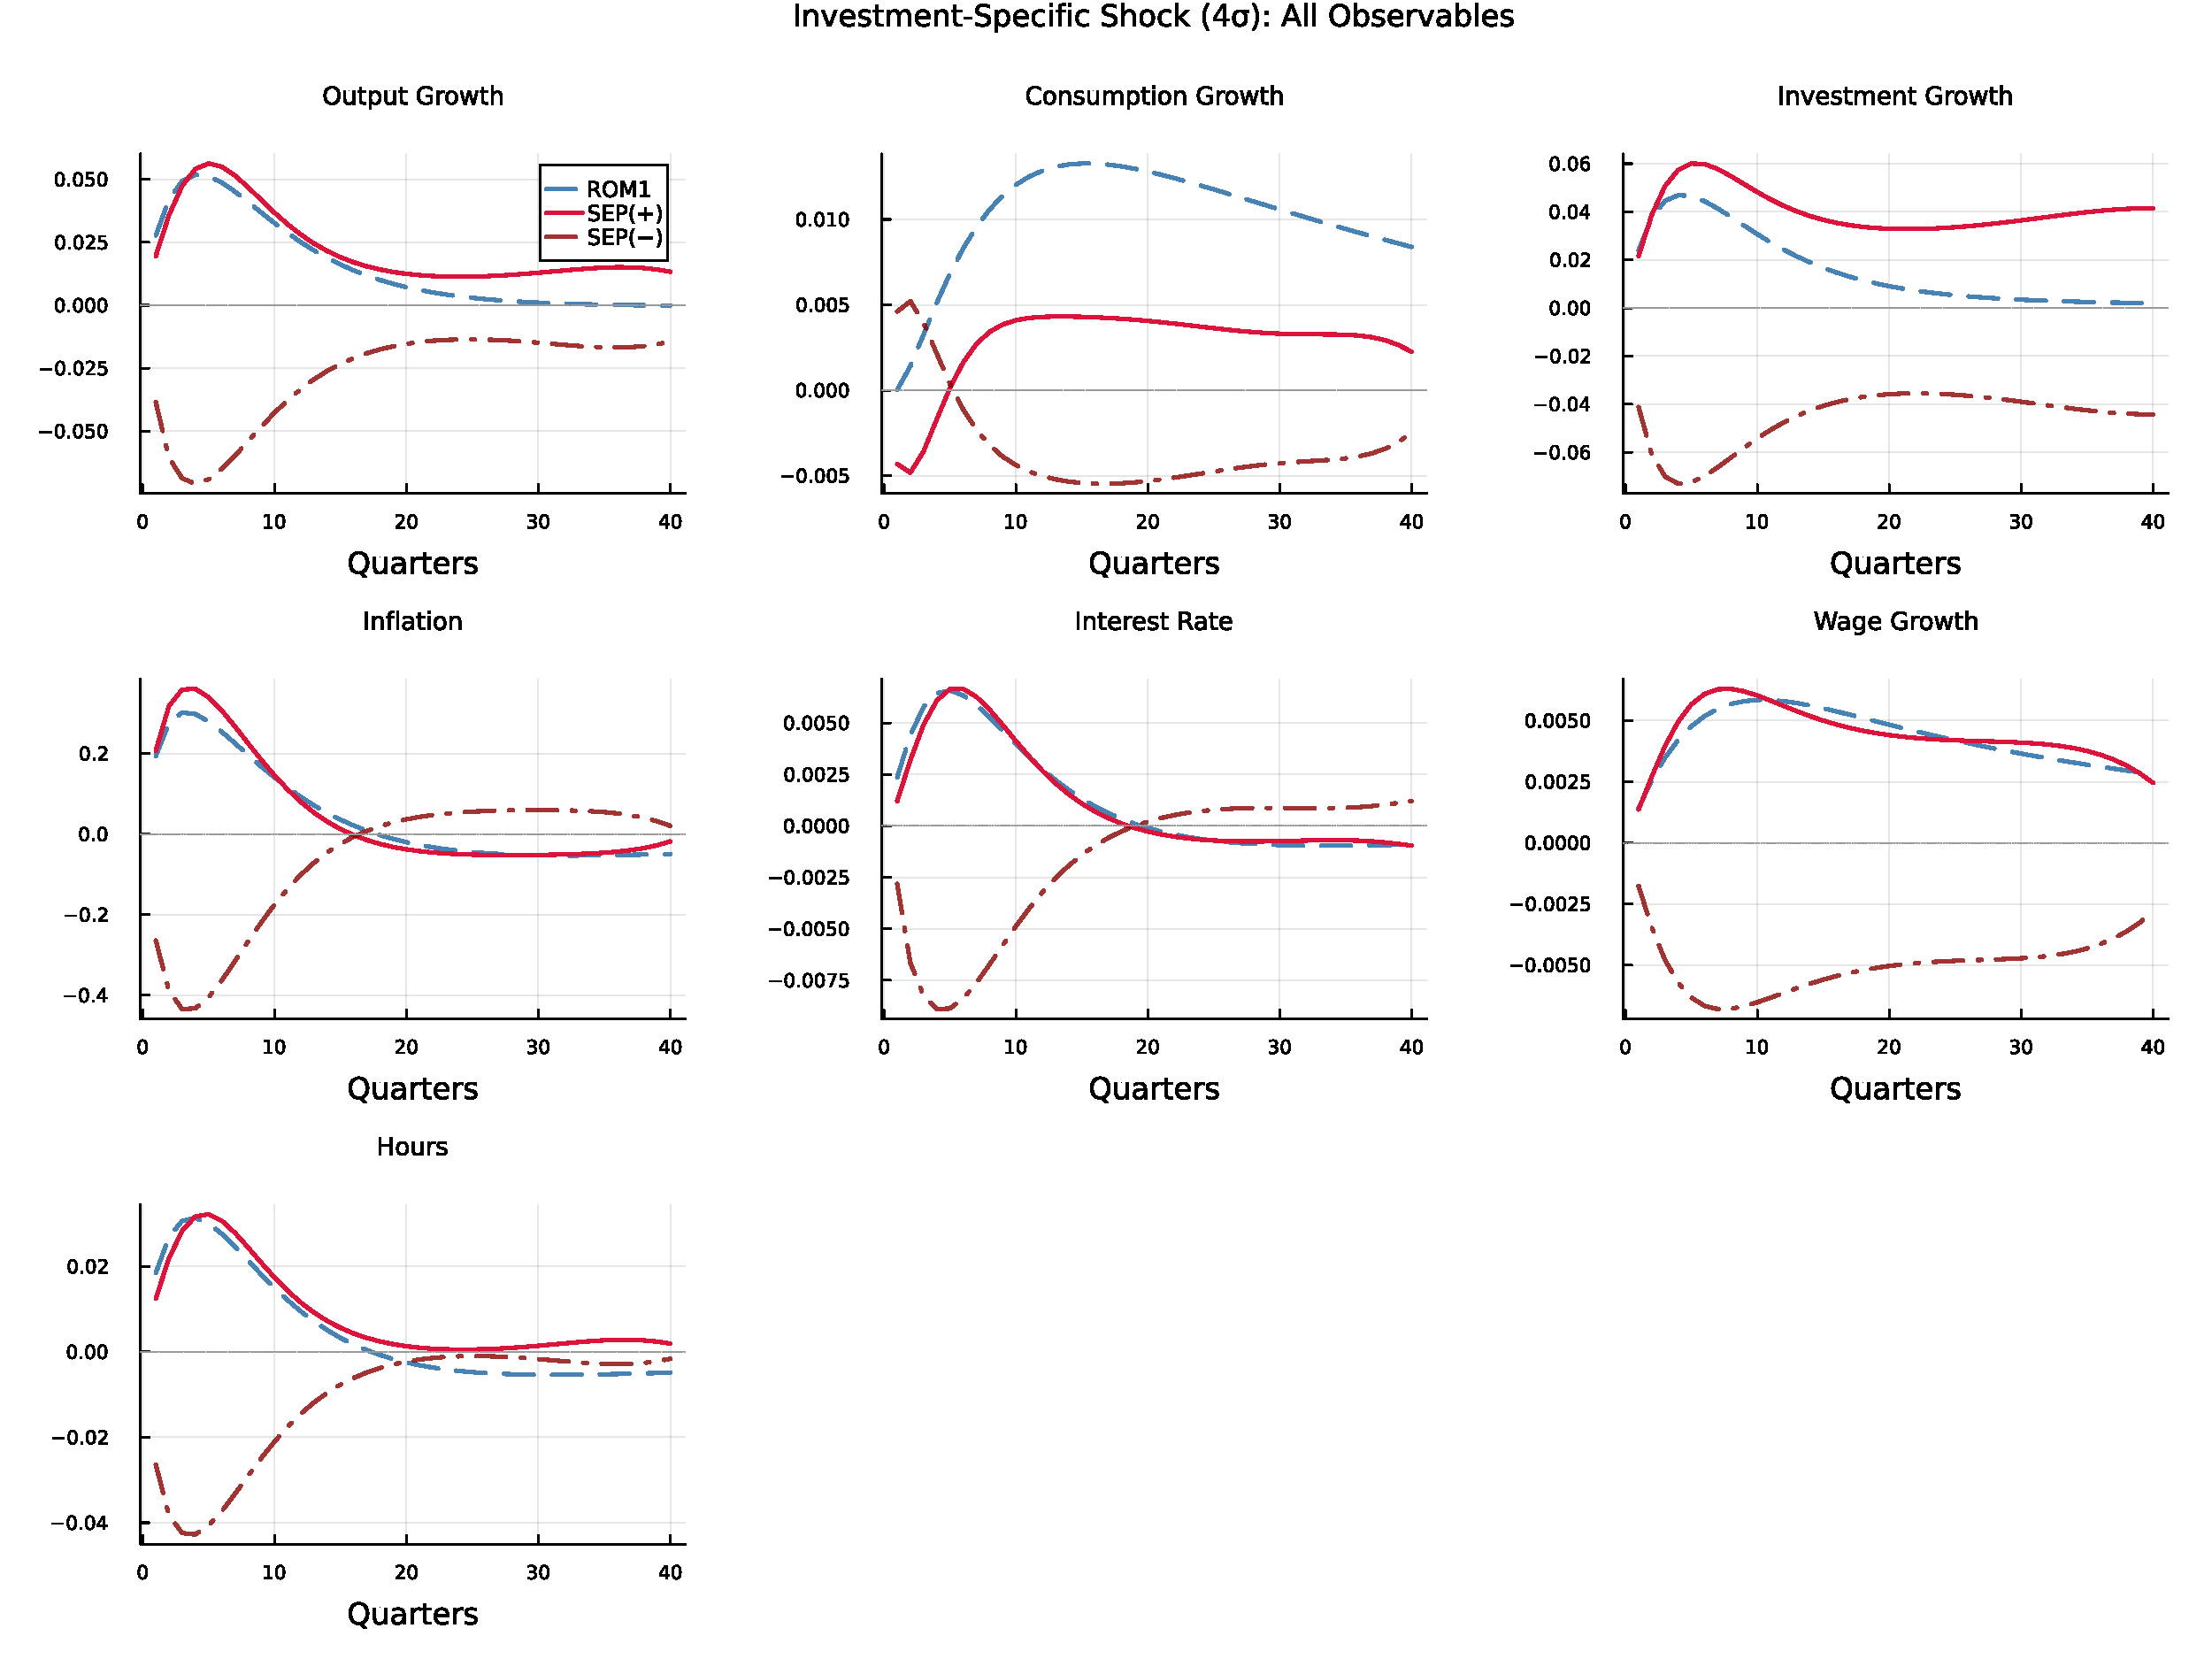
\includegraphics[width=\textwidth]{figures/fig_sep_all_vars_eqs_4sigma.pdf}
\caption{All-observable impulse responses to a $4\sigma$ investment-specific shock. ROM1 (blue dashed), SEP FOM positive (red solid), SEP FOM negative (dark red dash-dot). The nonlinear correction concentrates in investment growth, with spillovers to output and hours. Inflation and the interest rate are nearly unchanged between ROM1 and SEP FOM. Y-axis: percentage deviation from steady state.}
\label{fig:all_vars_eqs}
\end{figure}


\subsection{ROM1 Conditional-Prediction Errors in Real Data}
\label{subsec:rom1_forecast_errors}

Investment growth accounts for 53 percent of ROM1 one-step-ahead conditional-prediction error variance in U.S. data from 1959Q1 to 2004Q4 (Figure~\ref{fig:rom1_forecast_errors}, Table~\ref{tab:crisis_vs_normal}). During crisis quarters (13 of 184), investment RMSE jumps $6.3\times$ while inflation errors \emph{fall} ($0.83\times$)---an asymmetry consistent with the convex utilization cost $a(z)$.

\begin{figure}[t]
\centering
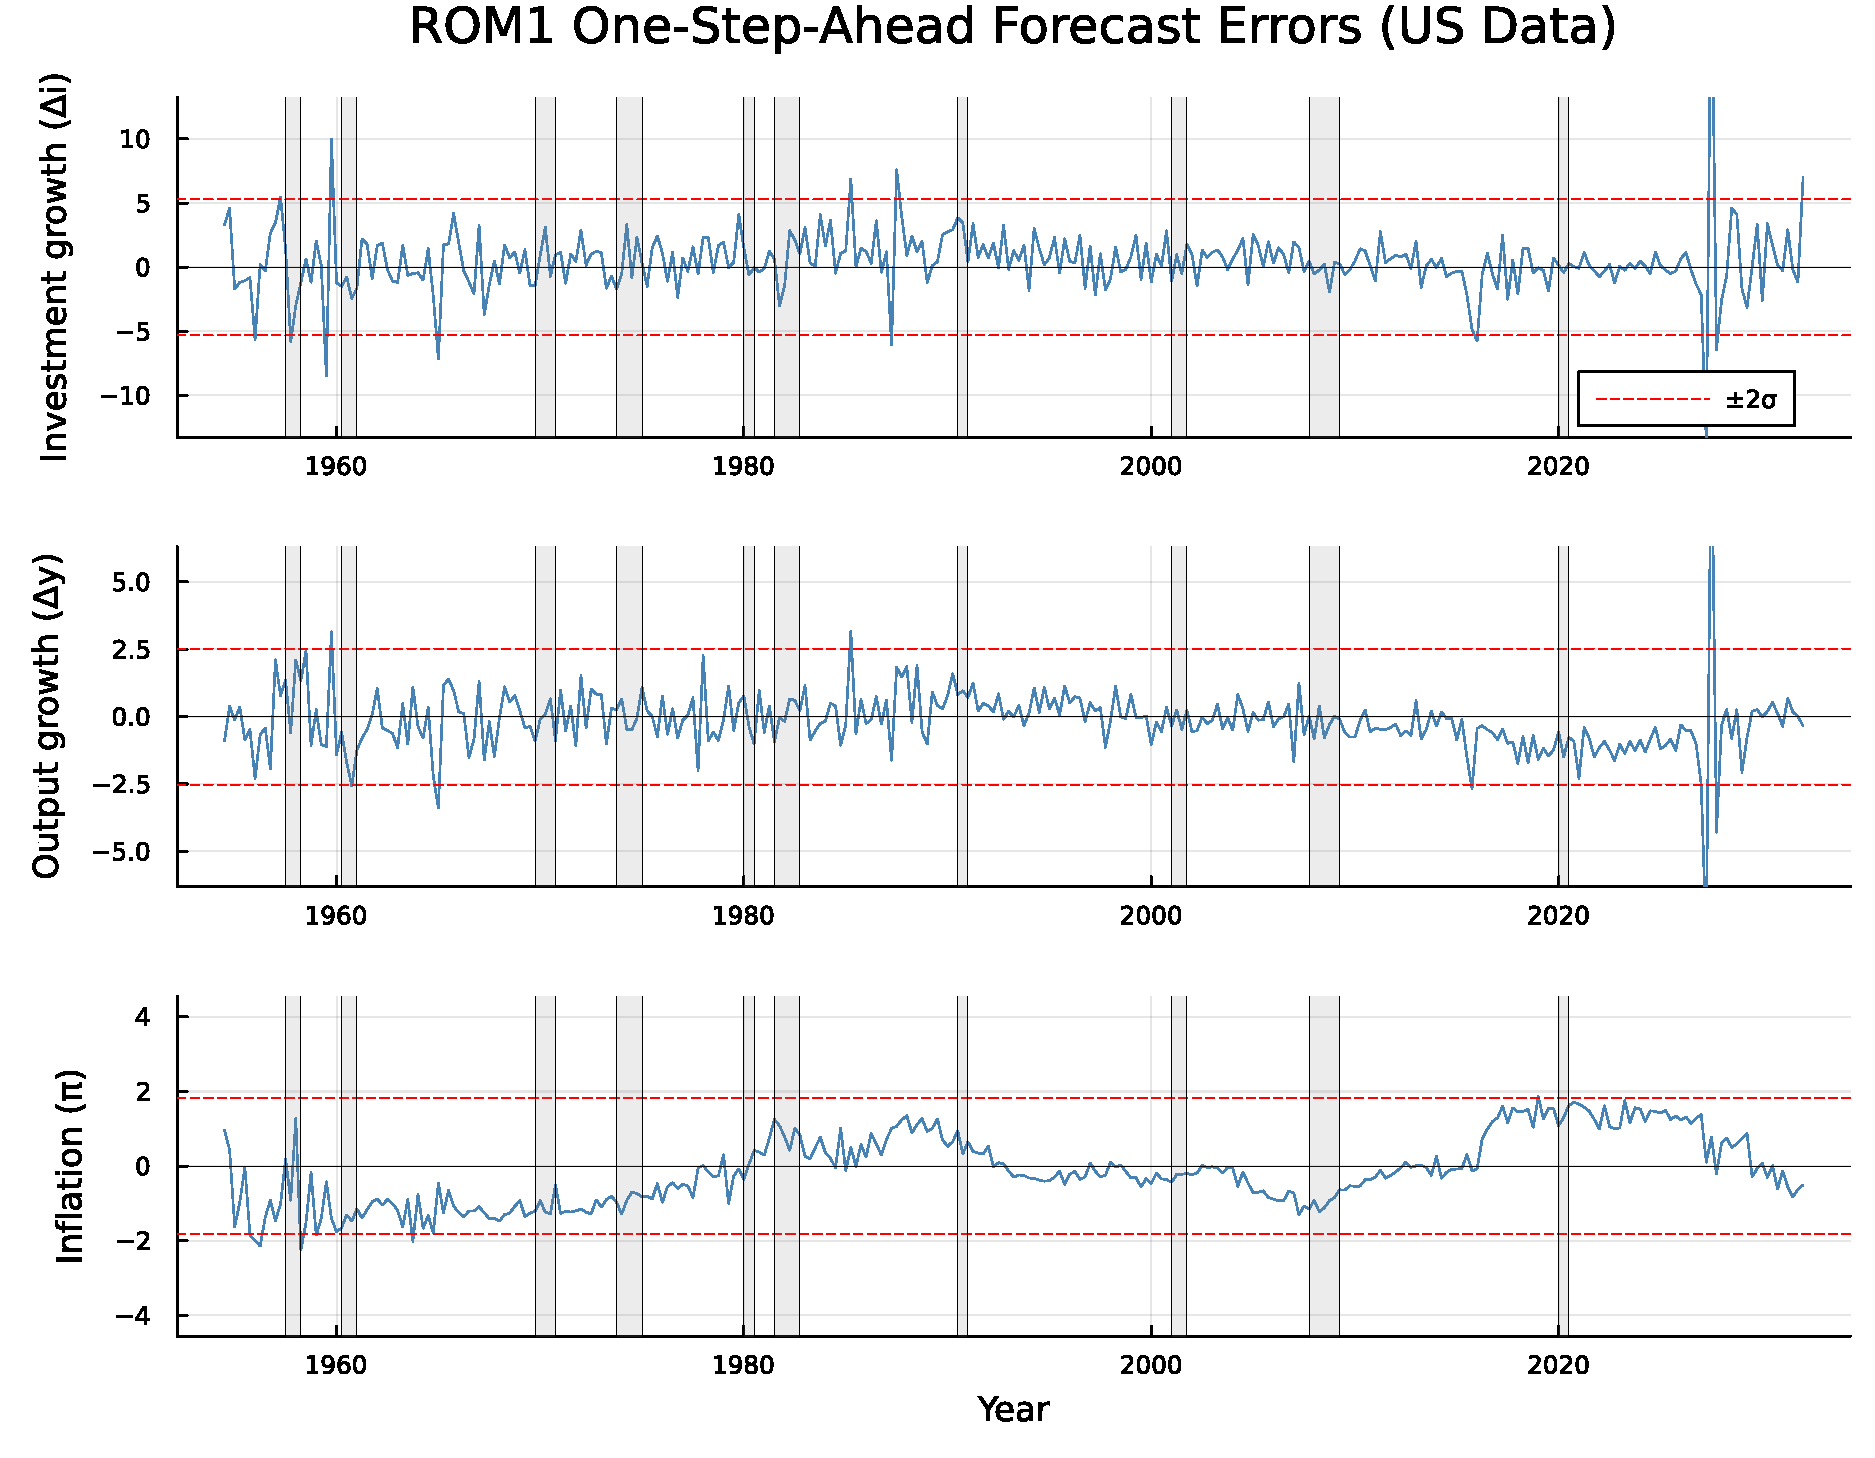
\includegraphics[width=\textwidth]{figures/fig_rom1_forecast_errors.pdf}
\caption{ROM1 one-step-ahead conditional-prediction errors for the real-data diagnostic sample, 1959Q1--2004Q4. Top: investment growth; middle: output growth; bottom: inflation. Errors are in the observable units used in estimation. Shaded areas: NBER recessions. Dashed red lines: $\pm 2\sigma$ bands computed from the full diagnostic sample.}
\label{fig:rom1_forecast_errors}
\end{figure}

\begin{table}[t]
\centering
\caption{ROM1 conditional-prediction errors: crisis vs.\ normal quarters}
\label{tab:crisis_vs_normal}
\begin{tabular}{lcccc}
\toprule
& \multicolumn{2}{c}{Forecast Error RMSE} & & \\
\cmidrule(lr){2-3}
Observable & Normal & Crisis & Ratio & Variance Share \\
\midrule
Investment growth ($\Delta i$) & 1.65 & 10.35 & 6.3$\times$ & 53.2\% \\
Output growth ($\Delta y$) & 0.88 & 4.48 & 5.1$\times$ & 12.1\% \\
Consumption growth ($\Delta c$) & 0.87 & 4.79 & 5.5$\times$ & --- \\
Hours worked & 0.59 & 1.68 & 2.8$\times$ & --- \\
Inflation ($\pi$) & 0.92 & 0.76 & 0.8$\times$ & 6.3\% \\
Wage growth ($\Delta w$) & 1.27 & 1.95 & 1.5$\times$ & --- \\
Interest rate ($r$) & 0.35 & 0.57 & 1.6$\times$ & --- \\
\bottomrule
\end{tabular}

\tablenotes{\textit{Notes}: Crisis quarters defined as periods where the absolute investment growth innovation exceeds $2\sigma$ of its unconditional standard deviation (13 out of 184 quarters, concentrated in the 1974--75, 1980--82, and 2001 recessions). Normal quarters are all remaining periods. Variance share is each observable's contribution to total one-step-ahead conditional-prediction error variance across all 184 quarters. ROM1 inversion filter applied to US quarterly data (1959Q1--2004Q4, 184 quarters) at calibrated \citet{smets2007shocks} parameter values.}
\end{table}

The decomposition measures transition-function gaps (69 percent from investment). The one-step prediction exercise measures data-fit failures (53 percent from investment). These are different objects---the numerical proximity is coincidental---but both point to the same channel. I therefore keep the benchmark comparison focused on the economically relevant choice in estimation practice: ROM1 versus the fully nonlinear SEP solution.


\subsection{The ELB as Alternative Hypothesis}
\label{subsec:elb_alternative}

If the ELB were the dominant nonlinearity, the investment-block share should decline when the constraint binds frequently. It does not in the plotted diagnostic. The investment block accounts for 89--92 percent of the total gap at every plotted shock scale from 0.8 to 1.5 (Figure~\ref{fig:decomposition_vs_scale}). The composition is flat across that plotted range, including the stress region where the gross-one floor first binds ($\geq 1.2\sigma$).

\begin{figure}[t]
\centering
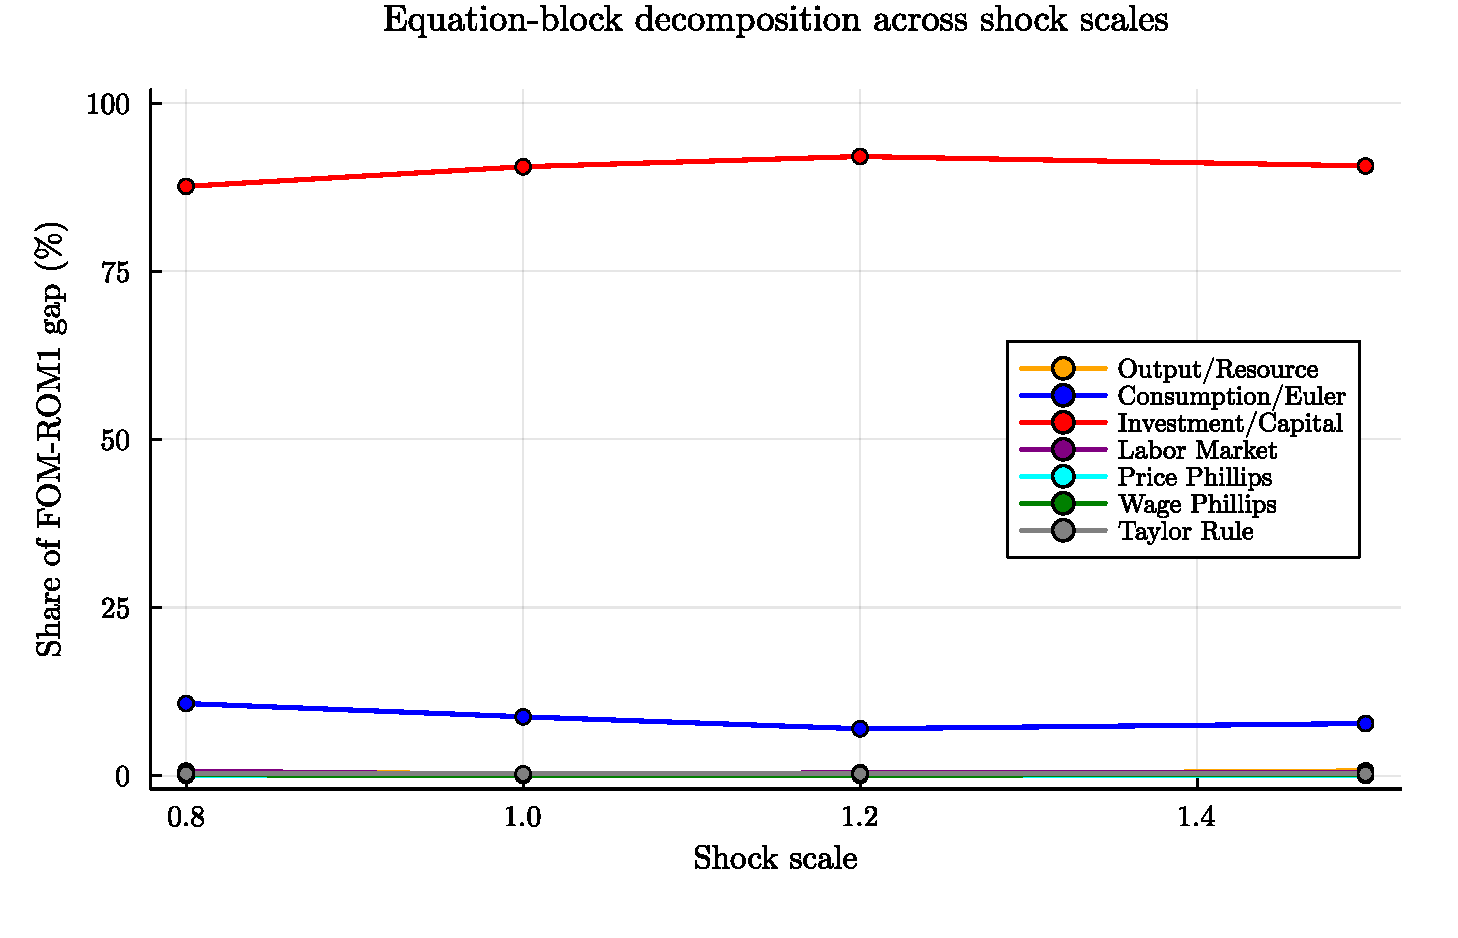
\includegraphics[width=\textwidth]{figures/decomposition_vs_shock_scale.pdf}
\caption{Equation-block decomposition of the FOM--ROM1 gap across the plotted shock-scale grid, 0.8--1.5. Each point is the average block share across ten Mahalanobis-stratified posterior draws and all simulated periods at that scale. Shares are percentages of the total squared transition-function gap. Investment/capital (red) holds at 89--92 percent across the plotted grid; the consumption/Euler block (blue) accounts for the remaining 8--11 percent. All other blocks are below 2 percent at every plotted scale.}
\label{fig:decomposition_vs_scale}
\end{figure}

In rare lower-bound-binding episodes the investment share falls---to 90 percent at shock scale 1.2 and 37 percent at scale 1.5. At posterior-estimated parameters, however, binding occurs in only 0.1--0.4 percent of periods, so the unconditional composition remains investment-dominated at 88--92 percent in this shock-scale diagnostic. That figure exceeds the training-set average of 69 percent because Sobol-sampled draws span parameter regions where the investment channel is weaker. Both exercises point the same way: investment dominates, and the ELB remains subordinate in this benchmark.


\subsection{Gal\'i Negative Control}
\label{subsec:gali_control}

The \citet{gali2015monetary} model is a negative-control comparison for the
lower-bound channel. It has Calvo pricing, a Taylor rule, and the same
lower-bound implementation used in the validation package, but it lacks investment
and capital. If the lower bound alone were the dominant source of the measured
SEP--ROM1 gap, this smaller model should show large gaps when the constraint
binds. It does not in the maintained shock-scale design.

The lower bound adds meaningful nonlinearity only above $3\sigma$ in this calibration
(Figure~\ref{fig:gali_obc_vs_no_obc}). At empirically relevant scales
($1$--$3\sigma$) the versions with and without the constraint are nearly
indistinguishable. At $10\sigma$ the lower bound quadruples the Gal\'i gap, but even
then the HLT gap remains seven to eight times larger.

\begin{figure}[t]
\centering
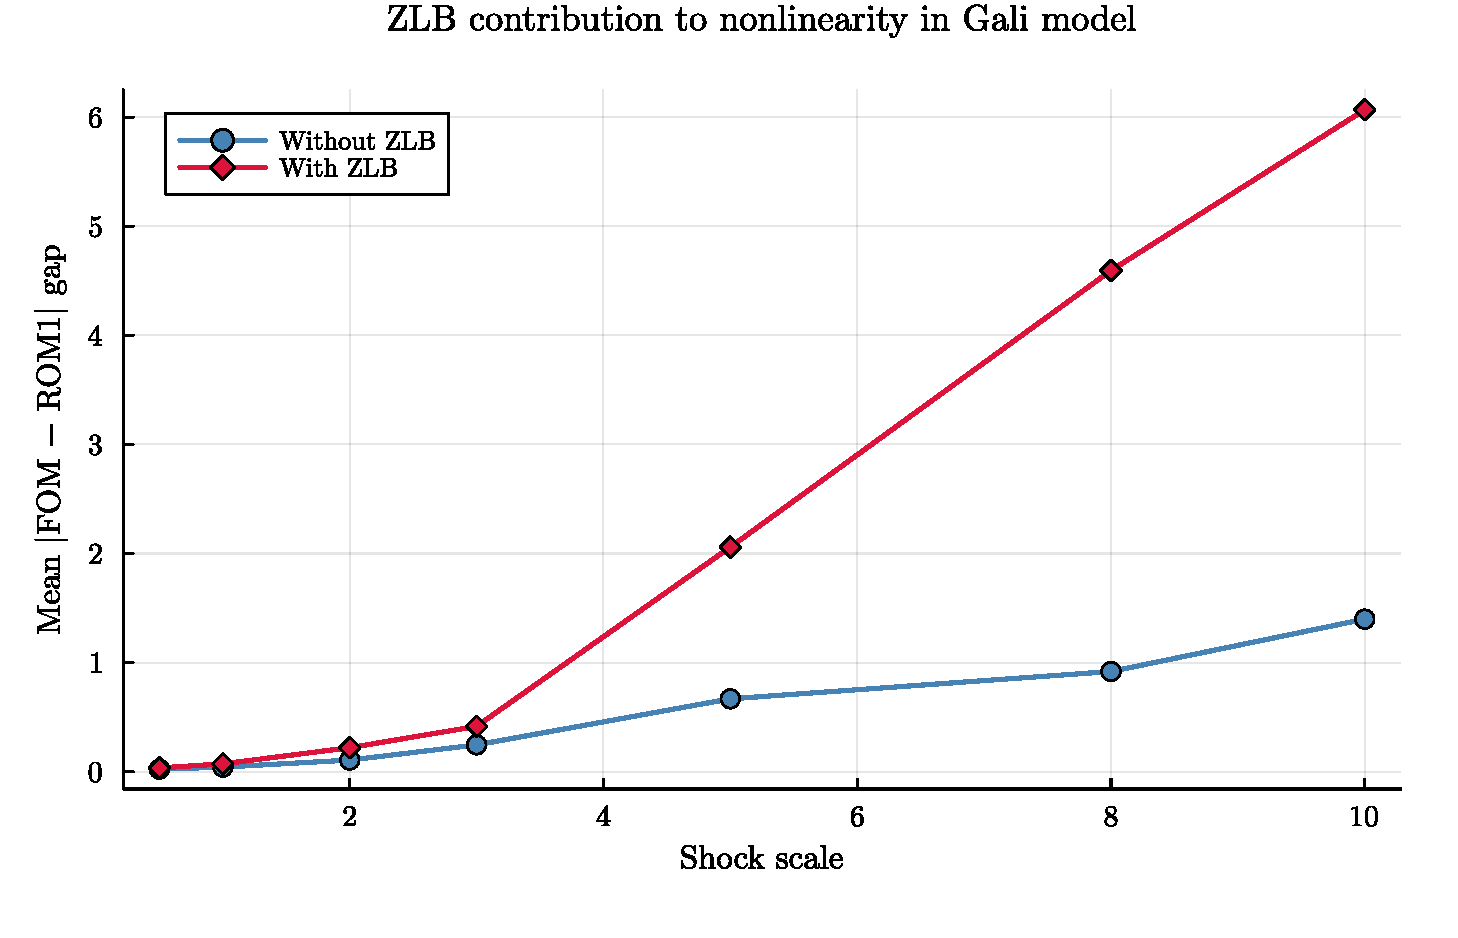
\includegraphics[width=0.85\textwidth]{figures/gali_obc_vs_no_obc.pdf}
\caption{Lower-bound contribution to nonlinearity in the Gal\'i model. Blue circles: FOM--ROM1 gap without the gross-one floor. Red diamonds: with the gross-one floor. The y-axis reports the mean absolute FOM--ROM1 transition gap in model units. Below $3\sigma$ shocks the two are nearly indistinguishable; the floor begins to matter at $5\sigma$ and roughly quadruples the gap at $10\sigma$. At empirically relevant shock scales in this calibration, the lower bound contributes negligibly to the FOM--ROM1 gap.}
\label{fig:gali_obc_vs_no_obc}
\end{figure}


\subsection{Counterfactual Model Variants}
\label{subsec:counterfactuals}

I construct three counterfactual models to assess the analytical hierarchy from Section~\ref{sec:invisibility}: one removes $S(\cdot)$ entirely, one replaces $a(z)$ with its first-order Taylor expansion, and one linearizes both.

Removing $S(\cdot)$ does not shrink the gap; in this counterfactual specification it grows 30--90 times larger over the reported shock-scale design. The adjustment cost both contributes to nonlinear marginal products and limits their magnitude by damping investment volatility. Without that convex friction, investment jumps freely, amplifying other nonlinearities through general equilibrium. Linearizing $a(z)$ alone changes the gap by less than 1.5 percent, suggesting that capital utilization nonlinearity is quantitatively small in this gap metric. The residual gap when both are linearized---from Tobin's~$q$ interactions, Kimball aggregation, and non-separable marginal utility---accounts for the 8--11 percent assigned to the consumption/Euler block in the plotted shock-scale grid (Figure~\ref{fig:decomposition_vs_scale}).


% ============================================================================
% CONSEQUENCES FOR INFERENCE
% ============================================================================

\section{Consequences for Inference}
\label{sec:inference_consequences}

The local validation harness exercises the HLT surrogate pipeline on synthetic data and includes a bounded direct SEP/MCMC comparison script for the HLT legacy three-parameter block. The repository also contains a Gal\'i ELB/OBC validation package that activates the ROM1-residual, inversion-filter, and matched-HMC layers: one-parameter smoke checks pass, and the two-parameter $(\sigma_z,\sigma_a)$ direct/surrogate HMC comparison passes on an actual-floor path. The package does not report the full three-shock direct-SEP HMC comparison, and the $\sigma_\nu$ probes behave as expected identification failures rather than surrogate-approximation failures. I therefore use the Gal\'i recovery exercises as pipeline diagnostics, not as main empirical evidence. I now turn to the 18-parameter estimation on U.S. data.

\subsection{18-Parameter Real-Data Estimation}
\label{subsec:results_18param_kalman}

I estimate the full 18-parameter HLT Smets--Wouters model on U.S. data (1959Q1--2004Q4, 184 quarters, 7 observables). The linear Kalman baseline uses 1,000 NUTS draws, has zero divergences, and takes 100 minutes.

\paragraph{Regime-switching surrogate estimation.}
\label{par:results_18param_switching}

The regime-switching gate classifies 10 percent of periods as nonlinear---concentrating around the Volcker disinflation, the early-1990s recession, and the dot-com bust---and completes in 2.4 hours with zero divergent transitions. The 18-nat profiled-hybrid-criterion gap ($-1{,}045$ vs.\ $-1{,}027$) is small relative to the objective scale itself.

Three parameter shifts in the reported HMC target are directionally consistent with the invisibility mechanism (Table~\ref{tab:18param_switching_posterior}).

\begin{enumerate}
\item \textbf{Risk-premium volatility doubles ($\sigma_b$: 0.12 $\to$ 0.28).} The linear model cannot generate the same state-dependent investment amplification as the nonlinear model. The parameter pattern is consistent with the linear specification using the exogenous risk-premium shock to fit investment volatility. Restoring the nonlinear $S_x \times p^k \times \xi_{t+1}/\xi_t$ channel is associated with $\sigma_b$ moving back toward its structural value.

\item \textbf{Wage markup persistence collapses ($\rho_w$: 0.37 $\to$ 0.08).} The linear model's posterior $\rho_w$ is comparable in magnitude to the persistence of the nonlinear propagation channel (autocorrelation 0.81, mean burst length 12.5 quarters), a pattern consistent with the linear model relying on persistent wage markup shocks where the nonlinear model uses state-dependent amplification. Restoring the nonlinear channel is associated with a reduction in exogenous persistence, though the absence of the ARMA(1,1) moving-average terms may also contribute to the low $\rho_w$ estimate. The baseline uncertainty from bimodality in $\rho_w$ (two linear chains find 0.39 vs.\ 0.75) means the magnitude should be interpreted cautiously.

\item \textbf{Kimball curvature rises 2.7-fold ($\varepsilon_p$: 39 $\to$ 104).} Higher $\varepsilon_p$ reduces nonlinearity by flattening demand. The linear posterior concentrates on low $\varepsilon_p$ while the regime-switching surrogate target settles at higher values, directionally consistent with the theory but occurring in a weakly identified region (the surrogate-target 90 percent interval [56.6, 149.6] covers much of the prior support). The sensitivity analysis in Section~\ref{subsec:csadjcost_sensitivity} supports the investment-dominance finding over $S''(1) \in [2, 10]$ in a bounded 25-draw design, with the investment share ranging from 89 to 95 percent.
\end{enumerate}

The 18-nat criterion gap means some shifts could partly reflect surrogate error and the profiled inversion objective. Two independent linear chains converge to modes separated by 34 nats, so shifts should be read as mode-specific. A direct SEP comparison at posterior draws shows that the ROM1--SEP prediction gap averages 1.04 RMSE per variable---well above the surrogate's training RMSE of 0.47---which supports the view that nonlinear solution differences are economically material at these parameter values.

\begin{table}[htbp]
\centering
\caption{Parameter Comparison: Kalman vs.\ Regime-Switching Surrogate}
\label{tab:18param_switching_posterior}
\begin{tabular}{llrrrr}
\toprule
Parameter & Description & Kalman & RS Surrogate & $\Delta$ & RS 90\% CI \\
\midrule
\multicolumn{6}{l}{\textit{Shock Persistence}} \\
$\rho_a$ & TFP & 0.987 & 0.980 & $-$0.007 & [0.965, 0.987] \\
$\rho_b$ & Risk premium & 0.762 & 0.590 & $-$0.172 & [0.220, 0.800] \\
$\rho_g$ & Government & 0.986 & 0.974 & $-$0.012 & [0.953, 0.988] \\
$\rho_{qs}$ & Investment & 0.782 & 0.818 & $+$0.036 & [0.709, 0.952] \\
$\rho_{\pi}$ & Price markup & 0.059 & 0.042 & $-$0.017 & [0.013, 0.109] \\
$\rho_w$ & Wage markup & 0.375 & 0.078 & $-$0.297 & [0.013, 0.343] \\
$\rho_{ms}$ & Monetary & 0.182 & 0.069 & $-$0.113 & [0.015, 0.189] \\
\midrule
\multicolumn{6}{l}{\textit{Shock Volatilities}} \\
$\sigma_a$ & TFP & 0.502 & 0.503 & $+$0.001 & [0.454, 0.564] \\
$\sigma_b$ & Risk premium & 0.122 & 0.275 & $+$0.153 & [0.113, 1.059] \\
$\sigma_g$ & Government & 0.508 & 0.513 & $+$0.005 & [0.461, 0.579] \\
$\sigma_{qs}$ & Investment & 0.361 & 0.353 & $-$0.008 & [0.288, 0.469] \\
$\sigma_{\pi}$ & Price markup & 0.143 & 0.147 & $+$0.004 & [0.125, 0.185] \\
$\sigma_w$ & Wage markup & 0.204 & 0.330 & $+$0.126 & [0.212, 0.406] \\
$\sigma_{ms}$ & Monetary & 0.245 & 0.248 & $+$0.003 & [0.221, 0.283] \\
\midrule
\multicolumn{6}{l}{\textit{Structural Parameters}} \\
$\xi_p$ & Calvo prices & 0.740 & 0.755 & $+$0.015 & [0.549, 0.894] \\
$\iota_p$ & Price indexation & 0.932 & 0.886 & $-$0.046 & [0.708, 0.962] \\
$\varepsilon_p$ & Kimball curvature & 39.3 & 104.2 & $+$64.9 & [56.6, 149.6] \\
$\xi_w$ & Calvo wages & 0.947 & 0.929 & $-$0.018 & [0.889, 0.946] \\
\bottomrule
\end{tabular}
\tablenotes{\textit{Notes}: ``Kalman'' column reports posterior means from a linear NUTS chain (1,000 draws, AdvancedHMC.jl, zero divergences, ESS $\geq 501$) initialized with the same seed as the RS chain. These values differ from an alternative-seed linear chain that converges to a different posterior mode (see convergence diagnostics in text). ``RS Surrogate'' reports means from the regime-switching NUTS chain (1,000 draws, zero divergences, 2.4 hours on Apple M4) targeting a profiled hybrid objective rather than an exact marginal likelihood. $\Delta$ is the difference in reported means. RS 90\% CI is the 5th--95th percentile interval from that HMC target. Shock volatilities are quarterly innovation standard deviations in the model's transformed observable scale. Criterion values at reported means: Kalman log likelihood $-1{,}027$; regime-switching profiled hybrid objective $-1{,}045$. Sample period: 1959Q1--2004Q4 ($T=184$ quarters).}
\end{table}

\paragraph{Convergence diagnostics.} Neither chain produces divergent transitions; within-chain ESS exceeds 501 (linear) and 473 (regime-switching). Two independent linear chains find different posterior modes---$\rho_w$ settles at 0.39 versus 0.75, with a 34-nat log-likelihood gap---indicating ridge-like posterior geometry in the wage/price markup block \citep{herbst2016sequential}. A second regime-switching chain initialized from a different point converges 12,700 nats below the primary chain, indicating severe multimodality in the profiled surrogate target. This is not unique to the surrogate: the 34-nat gap between linear chains shows that the SW07 posterior itself has ridge-like geometry. A multi-start protocol with parallel tempering \citep{herbst2019tempered} would systematically explore competing modes; the results here should be read as conditional on the primary mode.

\paragraph{Scope limitations.} The baseline training data use shock scale $\sigma = 0.1$, at which the lower bound rarely binds. A supplementary dataset at $\sigma = 0.4$ adds 20,240 lower-bound-binding samples, achieving RRMSE $= 0.12$ on binding episodes. The out-of-distribution (OOD) detection mechanism falls back to ROM1 for states outside the training envelope, but the surrogate's extrapolation behavior at intermediate out-of-distribution states remains a source of unquantified error. Section~\ref{subsec:extended_sample} extends both estimations through 2025Q1.

\subsection{Runtime}
\label{subsec:results_hlt_runtime}

Table~\ref{tab:benchmarks} compares computational costs. The regime-switching surrogate is about 20 times slower per evaluation than the Kalman filter, but orders of magnitude faster than a particle filter with nonlinear transitions.

\begin{table}[htbp]
\centering
\caption{Computational Benchmark Comparison}
\label{tab:benchmarks}
\resizebox{\textwidth}{!}{%
\begin{tabular}{lcccc}
\toprule
Method & Per Eval (s) & 1{,}000 NUTS Draws & Status & ESS/Divergences \\
\midrule
Kalman filter (ROM1) & 0.003 & 100 min & Complete & $\geq 501$ / 0 \\
Regime-switching surrogate & 0.06 & 2.4 hours & Complete & $\geq 473$ / 0 \\
Bootstrap PF + ROM1 ($N_p\!=\!5{,}000$) & 0.70 & $\approx 12$ min$^*$ & Evaluated$^\dagger$ & ESS $= 1.0$ \\
Bootstrap PF + SEP ($N_p\!=\!100$, 4 cores) & $\approx 3{,}700$ & $\approx 43$ days & Projected & --- \\
Bootstrap PF + SEP ($N_p\!=\!100$, 100 cores) & $\approx 147$ & $\approx 1.7$ days & Projected & --- \\
\bottomrule
\end{tabular}}
\tablenotes{\textit{Notes}: All timings on Apple M4 (single workstation, 4 performance cores). Kalman and RS surrogate rows are actual wall-clock times using AdvancedHMC.jl NUTS with finite-difference gradients. PF + SEP rows are projected assuming linear scaling. $^*$Per-evaluation cost only; MCMC would require tens of thousands of such evaluations. $^\dagger$Evaluated at the extended-sample posterior mean ($T=265$): ESS collapses to 1.0 in all 265 periods at every particle count tested ($N_p \in \{100, 500, 1{,}000, 5{,}000\}$), consistent with severe particle-weight degeneracy.}
\end{table}

A bootstrap particle filter \citep{gordon1993novel} collapses to a single effective particle in every period at all particle counts tested ($N_p$ up to $5{,}000$), producing a log-likelihood magnitude roughly four orders worse than the exact Kalman value at $N_p=5{,}000$ in the timing diagnostic. In a 7-dimensional observation space, the number of particles required for reliable importance sampling grows exponentially \citep{snyder2008obstacles}. Advanced particle filters---tempered \citep{herbst2019tempered}, conditionally optimal \citep{aruoba2021piecewise}---alleviate degeneracy in smaller models but remain far below the Kalman benchmark in the comparisons reported here. The filter-free formulation sidesteps this problem by treating shocks as explicit unknowns.

The offline cost of the surrogate is 12 hours (10 hours dataset generation, 2 hours training). The same residual surrogate serves multiple estimation runs without retraining, since the nonlinear-minus-linear transition residual $\Delta g_\theta(s, \varepsilon)$ does not depend on observed data. A 1,000-draw NUTS run achieves a $2{,}450\times$ speedup over direct SEP evaluation.


\subsection{Extended-Sample Estimation Through 2025}
\label{subsec:extended_sample}

The baseline sample excludes the episodes where nonlinear dynamics should matter most. I extend the estimation through 2025Q1 ($T = 265$ quarters), running both the linear NUTS-HMC and the regime-switching surrogate NUTS-HMC on the same extended dataset. No surrogate retraining is needed: the neural network maps from $(\text{state}, \text{shock}, \theta)$ to observation corrections, so it generalizes to any sample period as long as the state space remains within the training support.

Table~\ref{tab:extended_sample_posterior} reports the results. Under the linear Kalman filter, extending through 2025Q1 produces large COVID-driven shifts: shock volatilities rise ($\sigma_a$: 0.50 to 0.72, $\sigma_{qs}$: 0.36 to 0.52), investment persistence falls ($\rho_{qs}$: 0.78 to 0.65), and monetary persistence doubles ($\rho_{ms}$: 0.18 to 0.38)---reflecting the Federal Reserve's aggressive COVID-era response. The Kalman smoother at the linear posterior mean recovers risk-premium shocks of $56\sigma$ during 2020Q1--2021Q2 (Figure~\ref{fig:covid_shock_comparison}). These shock magnitudes are a diagnostic of model strain, not by themselves a proof that the profiled surrogate target is globally preferred.

The regime-switching surrogate improves the chain-mean profiled hybrid objective by 35.92 nats ($-1{,}781.68$ versus $-1{,}817.59$; pooled mean across four warm-started chains). This is a large criterion difference, but it is conditional on the high-objective warm-started mode, the surrogate approximation, the profiled inversion objective, the gate design, and the COVID window's out-of-distribution status. Within that profiled nonlinear objective, the fit is associated with lower estimated shock volatilities than the linear posterior mean. All seven shock volatilities fall: risk-premium volatility $\sigma_b$ drops 49 percent (0.179 to 0.092), investment volatility $\sigma_{qs}$ falls from 0.524 to 0.408, and TFP volatility $\sigma_a$ falls from 0.716 to 0.636. In exchange, persistence rises in the investment and wage blocks---$\rho_b$ from 0.731 to 0.899 and $\rho_w$ from 0.160 to 0.230.

The direction of the $\sigma_b$ shift reverses between the baseline and extended samples: $\sigma_b$ rises in the baseline (0.12 to 0.28) but falls here (0.18 to 0.09). The reversal is consistent with the risk-premium shock playing different roles across sample periods. In the baseline (1959--2004), which excludes extreme episodes, the nonlinear model's endogenous amplification is associated with $\sigma_b$ absorbing investment-driven variation that the linear model attributes to other shocks. In the extended sample, the COVID episode generates observations so extreme that the linear model inflates $\sigma_b$ dramatically (from 0.12 to 0.18); the nonlinear channel is then associated with lower $\sigma_b$ and higher persistence ($\rho_b$: 0.73 to 0.90). The cold-started surrogate chains do not find this high-objective basin, so the headline comparison should be stated as conditional on the warm-started mode unless a broader mode search measures posterior mass across basins.

The sampled target geometry is consistent with the decomposition but should be read as supporting evidence. Kimball curvature $\varepsilon_p$ rises from 82 to 121 but achieves a pooled effective sample size of only 90 draws across four warm-started chains---the target is nearly flat in that direction, consistent with the data providing little information about the pricing nonlinearity under this criterion. Risk-premium persistence $\rho_b$, which enters the investment Euler equation directly, achieves a pooled ESS of 4{,}434. The identification asymmetry---sharp identification on the investment-Euler parameters, near-flat target geometry on the pricing nonlinearity---matches the equation-block decomposition. The surrogate's validation error (RRMSE $= 0.0012$) is small relative to the ROM1--SEP gap, but the COVID extrapolation and gate design remain first-order caveats.

\begin{table}[htbp]
\centering
\caption{Extended-Sample Parameter Comparison (1959Q1--2025Q1)}
\label{tab:extended_sample_posterior}
\begin{tabular}{llrrrr}
\toprule
Parameter & Description & Kalman & RS Surrogate & $\Delta$ & RS 90\% CI \\
\midrule
\multicolumn{6}{l}{\textit{Shock Persistence}} \\
$\rho_a$ & TFP & 0.988 & 0.989 & $+$0.001 & [0.986, 0.990] \\
$\rho_b$ & Risk premium & 0.731 & 0.899 & $+$0.168 & [0.832, 0.945] \\
$\rho_g$ & Government & 0.986 & 0.987 & $+$0.000 & [0.980, 0.990] \\
$\rho_{qs}$ & Investment & 0.652 & 0.744 & $+$0.092 & [0.678, 0.792] \\
$\rho_{\pi}$ & Price markup & 0.021 & 0.020 & $-$0.001 & [0.011, 0.042] \\
$\rho_w$ & Wage markup & 0.160 & 0.230 & $+$0.070 & [0.130, 0.320] \\
$\rho_{ms}$ & Monetary & 0.376 & 0.304 & $-$0.072 & [0.196, 0.387] \\
\midrule
\multicolumn{6}{l}{\textit{Shock Volatilities}} \\
$\sigma_a$ & TFP & 0.716 & 0.636 & $-$0.080 & [0.592, 0.684] \\
$\sigma_b$ & Risk premium & 0.179 & 0.092 & $-$0.087 & [0.073, 0.116] \\
$\sigma_g$ & Government & 0.550 & 0.497 & $-$0.053 & [0.464, 0.534] \\
$\sigma_{qs}$ & Investment & 0.524 & 0.408 & $-$0.116 & [0.366, 0.468] \\
$\sigma_{\pi}$ & Price markup & 0.145 & 0.142 & $-$0.003 & [0.132, 0.154] \\
$\sigma_w$ & Wage markup & 0.367 & 0.334 & $-$0.033 & [0.293, 0.381] \\
$\sigma_{ms}$ & Monetary & 0.240 & 0.218 & $-$0.022 & [0.203, 0.235] \\
\midrule
\multicolumn{6}{l}{\textit{Structural Parameters}} \\
$\xi_p$ & Calvo prices & 0.938 & 0.940 & $+$0.002 & [0.921, 0.950] \\
$\iota_p$ & Price indexation & 0.961 & 0.900 & $-$0.061 & [0.842, 0.971] \\
$\varepsilon_p$ & Kimball curvature & 81.6 & 121.1 & $+$39.5 & [86.4, 136.6] \\
$\xi_w$ & Calvo wages & 0.945 & 0.946 & $+$0.001 & [0.938, 0.950] \\
\bottomrule
\end{tabular}
\tablenotes{\textit{Notes}: Extended sample 1959Q1--2025Q1 ($T=265$). ``Kalman'' reports posterior means from linear NUTS-HMC (2,000 draws, AdvancedHMC.jl, zero divergences, ESS $\geq 668$). ``RS Surrogate'' pools 8{,}000 post-warmup draws from four warm-started NUTS-HMC chains (seeds 42, 5, 6, 7; 2{,}000 draws per chain) with soft gating and zero divergences across all chains; pooled ESS $\geq 90$. The RS target is a profiled hybrid objective, not an exact marginal likelihood. $\Delta$ is the shift in reported means. RS 90\% CI is the 5th--95th percentile of the pooled draws from that target. Shock volatilities are quarterly innovation standard deviations in the model's transformed observable scale. Criterion values at reported means: Kalman log likelihood $-1{,}817.59$; RS profiled hybrid objective $-1{,}781.68$ (gap $35.92$ nats). Per-chain surrogate mean objectives range from $-1{,}787.38$ to $-1{,}780.80$.}
\end{table}

\begin{figure}[t]
\centering
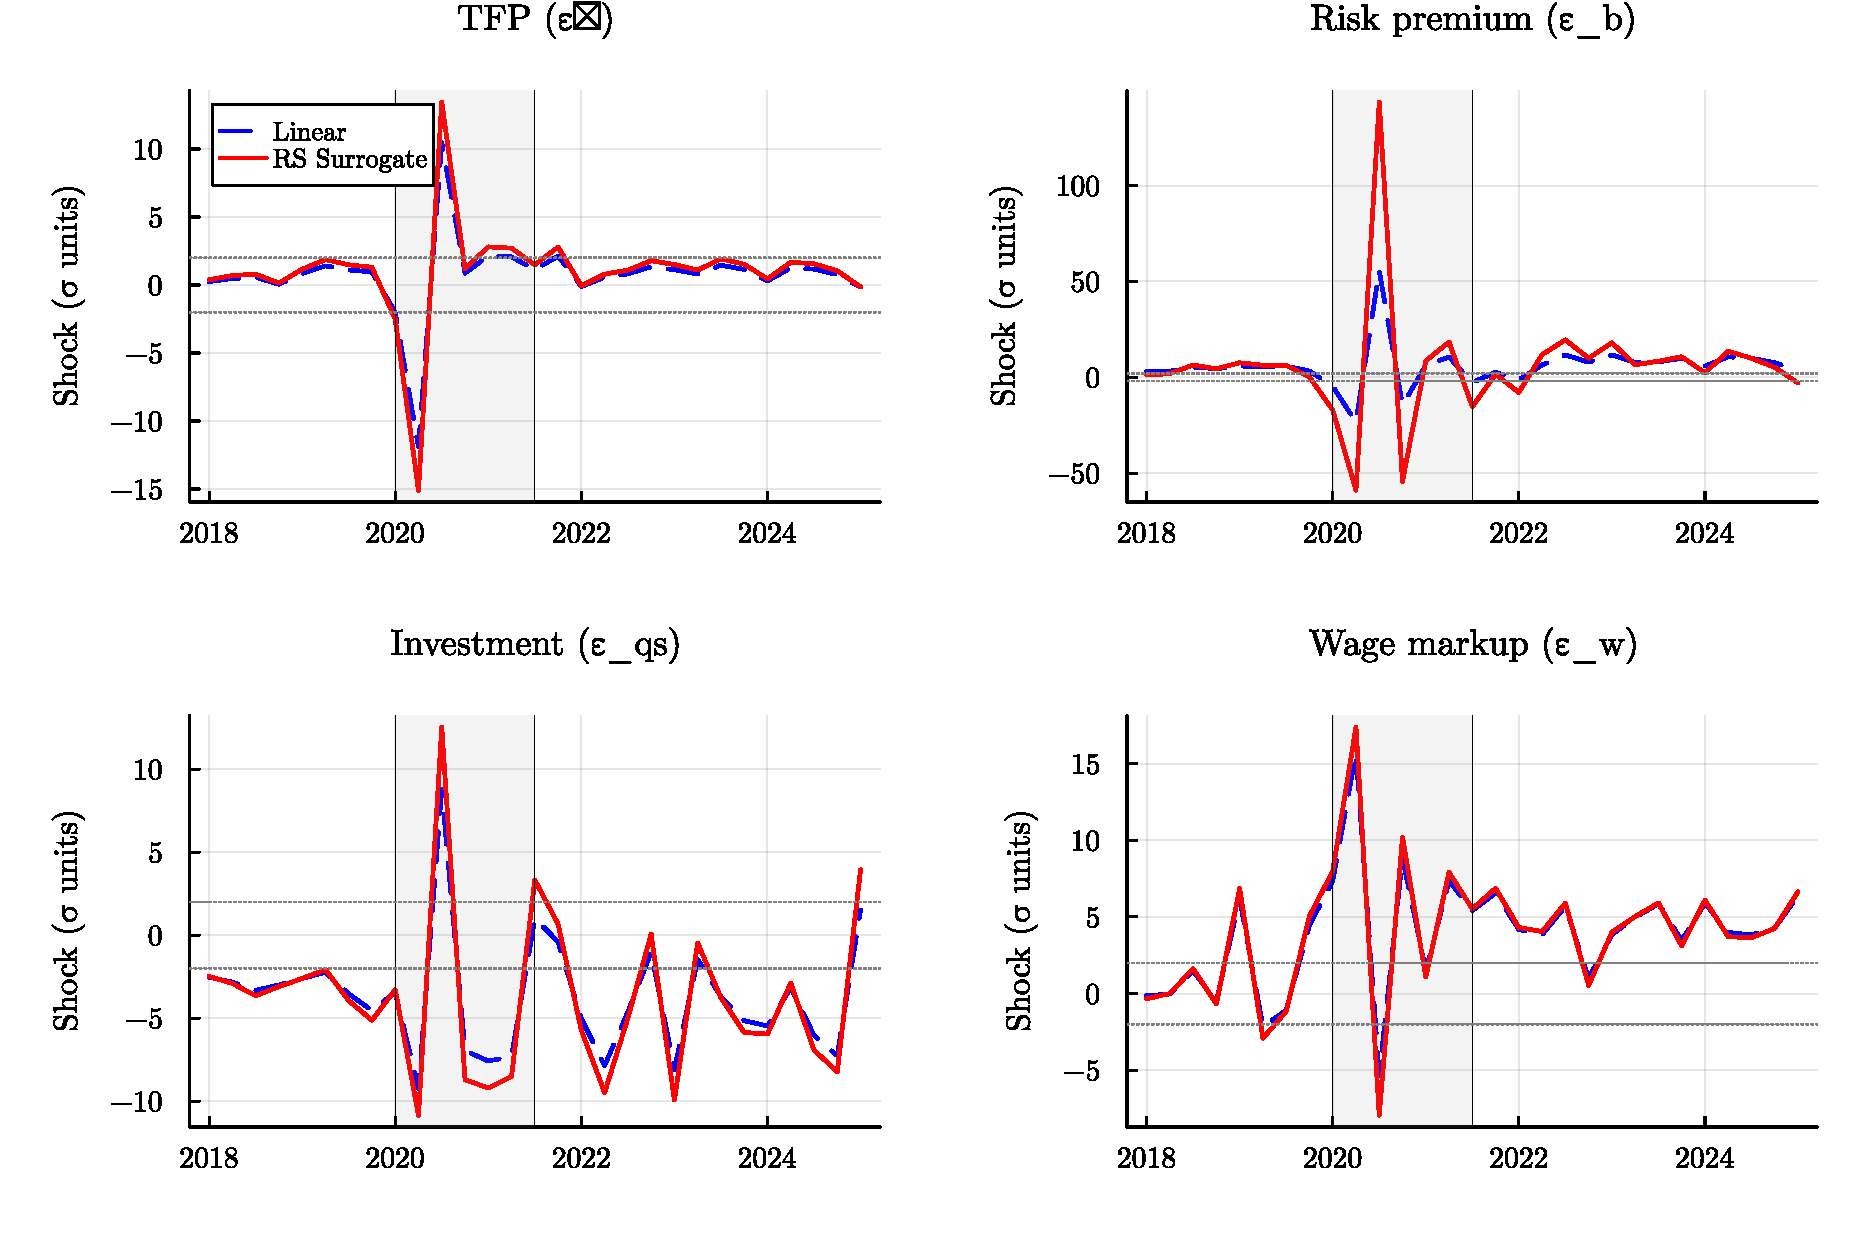
\includegraphics[width=0.95\textwidth]{figures/covid_shock_comparison.pdf}
\caption{Kalman-smoothed shocks (in $\sigma$ units), 2018--2025. Both series are evaluated through the same linear Kalman smoother; only the parameter vector differs. Blue dashed: linear posterior mean; red solid: regime-switching surrogate target mean. Gray band: COVID window (2020Q1--2021Q2). At the linear posterior, risk-premium shocks peak at $56\sigma$. At the surrogate target mean, the lower $\sigma_b$ can force even larger normalized shocks under a linear filter, illustrating that the surrogate parameters should be interpreted through the regime-switching profiled objective rather than through the Kalman smoother.}
\label{fig:covid_shock_comparison}
\end{figure}

\paragraph{Decomposing the Criterion Gap.}
A natural objection is that the 35.92-nat improvement might reflect parameter relocation rather than the nonlinear correction: could the linear model close the gap if its shocks were re-tuned to the surrogate's preferred parameter values? Concretely, how much of $\Delta Q = Q_{\text{surr}}(\hat{\theta}_{\text{surr}}) - Q_{\text{lin}}(\hat{\theta}_{\text{lin}})$ comes from the criterion change at fixed $\theta$, and how much from re-optimizing $\theta$ under the new criterion? I evaluate the four cells of the 2$\times$2 criterion table at the two posterior means.
Table~\ref{tab:ll_decomposition} reports this cross-evaluation.

\begin{table}[htbp]
\centering
\caption{Cross-evaluated log criteria at the linear posterior mean and surrogate target mean (extended sample, $T=265$).}
\label{tab:ll_decomposition}
\begin{tabular}{lcc}
\toprule
& $\hat{\theta}_{\text{lin}}$ & $\hat{\theta}_{\text{surr}}$ \\
\midrule
$Q_{\text{lin}}$ (Kalman likelihood)            & $-1{,}817.59$ & $-1{,}852.63$ \\
$Q_{\text{surr}}$ (regime-switching objective) & $-1{,}830.44$ & $-1{,}781.68$ \\
\bottomrule
\end{tabular}
\smallskip
\tablenotes{\textit{Notes}: $\hat{\theta}_{\text{lin}}$ is the linear NUTS-HMC posterior mean (extended sample, 2{,}000 draws); $\hat{\theta}_{\text{surr}}$ is the pooled mean across four warm-started surrogate chains. Kalman cells are exact log-likelihood evaluations; surrogate cells are profiled hybrid objectives on the same data and omit the shock-prior and determinant/Laplace terms required for a marginal-likelihood comparison.}
\end{table}

The off-diagonal entries provide a chain-mean accounting exercise. At $\hat{\theta}_{\text{surr}}$, the linear Kalman likelihood falls by 35.04 nats relative to its own posterior mean ($-1{,}852.63$ versus $-1{,}817.59$): the linear model does not absorb the surrogate's parameters. At $\hat{\theta}_{\text{lin}}$, the surrogate objective is 12.85 nats below the linear posterior-mean likelihood---swapping criteria without re-tuning loses ground because each parameter vector is fitted to its own criterion. Symmetrically averaging the two path decompositions of the gap (model-change-then-parameters and parameters-then-model-change) assigns 29.05 nats (80.9 percent) to the criterion change and 6.86 nats (19.1 percent) to parameter relocation. This is consistent with the nonlinear correction being the main source of the criterion gain within the high-objective surrogate mode, but it is an accounting exercise, not a likelihood decomposition or model-selection statistic.

The remaining design concern is whether the gain comes from the gate/inversion architecture itself rather than from the learned nonlinear residual. I therefore evaluate a fixed-parameter ablation that keeps the same gate, inversion filter, observation scaling, and soft criterion mixing, but sets the NN residual correction to zero. Table~\ref{tab:linear_gate_ablation} reports this no-NN objective at the same two chain means. The gate/inversion architecture alone lowers the criterion at both parameter vectors; the NN residual correction is what produces the positive gain. Symmetrically averaging across the two fixed parameter vectors gives a $-18.22$-nat gate/inversion contribution and a $+47.28$-nat NN-residual contribution. This fixed-parameter ablation does not replace a dedicated no-NN HMC chain, but it provides evidence against the simplest fixed-parameter version of the concern that the 35.92-nat result is mechanically generated by the gate or inversion filter.

\begin{table}[htbp]
\centering
\caption{Fixed-parameter ablation: gate/inversion architecture versus NN residual.}
\label{tab:linear_gate_ablation}
\begin{tabular}{lcc}
\toprule
& $\hat{\theta}_{\text{lin}}$ & $\hat{\theta}_{\text{surr}}$ \\
\midrule
$Q_{\text{lin}}$ (Kalman likelihood) & $-1{,}817.59$ & $-1{,}852.63$ \\
$Q_{\text{gate}}$ (gate+inversion, no NN) & $-1{,}845.10$ & $-1{,}861.57$ \\
$Q_{\text{surr}}$ (gate+inversion+NN) & $-1{,}830.44$ & $-1{,}781.68$ \\
\midrule
Gate/inversion gain over Kalman & $-27.51$ & $-8.94$ \\
NN residual gain over gate-only & $+14.66$ & $+79.89$ \\
\bottomrule
\end{tabular}
\smallskip
\tablenotes{\textit{Notes}: Fixed-parameter criterion evaluations on the extended sample. The no-NN row uses the same soft gate and inversion-filter objective as the surrogate row but zeros the neural residual correction. A full posterior or target-level ablation requires rerunning HMC with \texttt{--disable-nn-correction=true}.}
\end{table}

The extended-sample results are directionally consistent with the decomposition predictions. The theory predicts that the linear model's estimated shock processes may be inflated relative to the nonlinear model when the missing investment-channel amplification is quantitatively important. The baseline estimation on 1959--2004 is consistent with this qualitatively for some margins, though $\sigma_b$ rises rather than falls in the baseline; extending through 2025 provides a more demanding test where the direction of the $\sigma_b$ shift aligns with the prediction. The COVID window generates observations that the linear posterior mean rationalizes only with extreme shock realizations. The regime-switching surrogate achieves a higher profiled hybrid objective with smaller estimated shock volatilities, with the largest reduction in $\sigma_b$ ($-49$ percent)---the shock that feeds most directly into the investment Euler equation.

The decomposition identifies investment as the dominant nonlinearity source (69 percent); the criterion-based estimation independently finds that risk-premium dynamics are where linear and regime-switching surrogate targets diverge most. These two results---one deterministic, one criterion-based empirical---are consistent with the same underlying channel, approached from different angles.


\section{Discussion and Robustness}
\label{sec:robustness}

Initial-state treatment is not used as a headline validation result here. Any posterior-recovery claim for $s_0$ should be reported only after the Gal\'i direct SEP-HMC versus surrogate-HMC comparison is generated.

Surrogate accuracy is strong in the non-binding validation design but weaker in the lower-bound stress region. Across most parameter regions the held-out RRMSE is below 0.002, while the far-tail 95th percentile is 0.00231. The combined surrogate (63,939 samples including 20,240 lower-bound-binding episodes at shock scale 0.4) achieves RRMSE of 0.12 on binding-period test data---an 89 percent improvement over the version trained without lower-bound episodes, but much larger than the non-binding validation error. Gal\'i seed and prior sensitivity tables are excluded because the present validation evidence comes from the ELB/OBC package summarized in the online technical appendix.

During lower-bound-binding episodes, ROM1 predicts deeply negative rates; the surrogate adds back the approximate lower-bound correction and tracks the SEP benchmark qualitatively across the reported validation observables.

\subsection{Robustness to Pricing Specification}
\label{subsec:pricing_robustness}

The baseline Calvo pricing block produces only 0.2 percent of the FOM--ROM1 gap. A natural question is whether this finding reflects the Calvo specification itself rather than a generic property of pricing nonlinearity. I test three alternatives following the slope calibrations in \citet{alvarez2024rise}: (i) a high-slope variant matching the \citet{golosov2007menu} menu-cost model ($\kappa \approx 1.71$, $\xi_p = 0.034$), (ii) a moderate-slope variant matching \citet{nakamura2010monetary} ($\kappa \approx 0.47$, $\xi_p = 0.17$), and (iii) \citet{rotemberg1982sticky} quadratic adjustment-cost pricing, which introduces explicit $\pi^2$ nonlinearity in the resource constraint. All three variants maintain the identical investment, wage, and monetary policy blocks; only the pricing technology differs.

The Golosov--Lucas and Nakamura--Steinsson variants set the Kimball curvature $\varepsilon_p = 1$ (CES aggregation, matching the demand structure underlying the ARRS slope estimates) and adjust the Calvo probability $\xi_p$ to match each model's implied slope. The Rotemberg variant replaces the entire Calvo pricing block---eliminating seven auxiliary variables (price dispersion, reset ratios, and recursive pricing sums)---with a single nonlinear Phillips curve $\phi_R \pi_t (\pi_t - \bar{\pi}) = (1 - \varepsilon) + \varepsilon \, mc_t \, s_t^{\pi} + \beta \gamma^{-\sigma} E_t [\xi_{t+1}/\xi_t \cdot \phi_R \pi_{t+1} (\pi_{t+1} - \bar{\pi}) \cdot y_{t+1}/y_t]$, where $\varepsilon = \lambda_p / (\lambda_p - 1)$ is the demand elasticity (with $\lambda_p$ the gross steady-state price markup), and adds the quadratic adjustment cost $\frac{\phi_R}{2}(\pi_t - \bar{\pi})^2 y_t$ to the resource constraint. The adjustment cost $\phi_R$ is calibrated to match the baseline Calvo slope at $\xi_p = 0.6$. \citet{richter2016zlb} find mixed macro evidence for Rotemberg versus Calvo pricing; the present result---that the pricing block is small in each of the three pricing variants considered here---is consistent with their view that the two specifications are empirically close at first order.

The Golosov--Lucas and Nakamura--Steinsson variants produce block shares identical to the baseline: investment accounts for 89--91 percent of the gap, the price Phillips block for 0.0 percent. This is expected---changing $\xi_p$ and $\varepsilon_p$ alters the \emph{slope} of the linearized Phillips curve but does not materially change its nonlinear contribution in these three pricing variants.

The Rotemberg variant is the informative test. The quadratic adjustment cost $\frac{\phi_R}{2}(\pi_t - \bar{\pi})^2 y_t$ introduces explicit nonlinearity that is \emph{not} invisible---it has a nonzero second derivative at steady state. Even so, the investment block remains dominant at 83--86 percent, while the price Phillips share rises to at most 0.4 percent. Inflation deviations from trend are small relative to investment growth-rate deviations, so the Rotemberg cost generates minimal gap even though it is structurally visible. These results hold at shock scales from 0.1 through 1.0.

\subsection{Sensitivity to Investment Adjustment Cost Curvature}
\label{subsec:csadjcost_sensitivity}

The baseline calibration $S''(1) = 6.0$ follows \citet{smets2007shocks}. Since the 69 percent investment-dominance finding could in principle depend on this calibration, I re-run the equation-block decomposition at $S''(1) \in \{2, 4, 6, 8, 10\}$, spanning the range commonly used in the literature \citep{christiano2005nominal,justiniano2010investment}. At each value, I draw 25 representative parameter vectors from the surrogate posterior, simulate 40-period trajectories via SEP at unit shock scale, and compute the FOM--ROM1 gap decomposition.

Table~\ref{tab:csadjcost_sensitivity} reports the results. Investment dominance is stable in this design: the investment/capital block accounts for 89--95 percent of the gap across the full range, with lower curvature producing \emph{higher} investment shares ($S''(1) = 2$: 95.1\%) because the investment Euler equation becomes more nonlinear when the adjustment cost is less convex. The price Phillips curve contributes 0.0 percent at every calibration. The absolute gap magnitude declines monotonically with $S''(1)$ (from 5.6 to 2.8 model units), consistent with higher curvature suppressing investment volatility and thus reducing the scope for nonlinear amplification. All 25 parameter draws converge at every calibration point.

The stability of the relative shares supports the view that investment dominance is tied to the adjustment-cost mechanism rather than to a single baseline calibration. The curvature $S''(1)$ controls the \emph{magnitude} of the nonlinear gap more than its \emph{composition} in this 25-draw, 40-period sensitivity design; other equation blocks do not scale similarly with $S''(1)$ because their nonlinear terms (Kimball demand, capacity utilization) operate through different channels.

% S''(1) sensitivity analysis — equation-block decomposition
% Generated: 2026-04-21T11:59:57.099
\begin{table}[htbp]
\centering
\caption{Equation-Block Decomposition: Sensitivity to $S''(1)$}
\label{tab:csadjcost_sensitivity}
\begin{tabular}{lcccccccc}
\toprule
$S''(1)$ & Investment & Consumption & Output & Labor & Price & Wage & Taylor & Gap \\
\midrule
2.0 & 95.1 & 4.5 & 0.2 & 0.1 & 0.0 & 0.0 & 0.1 & 5.6044 \\
4.0 & 94.1 & 5.5 & 0.1 & 0.1 & 0.0 & 0.0 & 0.2 & 3.6844 \\
\textbf{6.0} & 92.2 & 7.3 & 0.1 & 0.1 & 0.0 & 0.0 & 0.3 & 3.6558 \\
8.0 & 91.8 & 7.5 & 0.1 & 0.2 & 0.0 & 0.0 & 0.3 & 2.7908 \\
10.0 & 88.8 & 10.2 & 0.3 & 0.3 & 0.0 & 0.0 & 0.4 & 2.7618 \\
\bottomrule
\end{tabular}
\begin{minipage}{0.92\textwidth}
\footnotesize\textit{Notes:} Each column reports the share of the mean squared FOM--ROM1 gap attributable to the corresponding equation block, expressed as a percentage. ``Gap'' reports the root-mean-square observable gap in model units. The baseline calibration $S''(1) = 6.0$ is shown in bold. Shares sum to 100\% by construction (orthogonal decomposition). 25 representative parameter vectors drawn from the posterior; 40 periods per trajectory at unit shock scale.
\end{minipage}
\end{table}


\subsection{Known Limitations}
\label{subsec:known_limitations}

Two independent linear chains find different posterior modes (34-nat gap), indicating ridge-like posterior geometry in the wage/price markup block \citep{herbst2016sequential}. The decomposition results are deterministic and unaffected; the parameter comparisons in Section~\ref{sec:inference_consequences} are conditional on a single mode and on the profiled inversion objective used for the surrogate cells.

The baseline surrogate is trained at shock scale 0.1, where the lower bound rarely binds; the supplementary dataset at scale 0.4 extends coverage to binding episodes. The same surrogate can be evaluated on different sample periods without retraining because the neural network maps from parameter-state-shock space rather than time-series indices, but this does not eliminate out-of-distribution risk. The active validation record should be read as bounded support evidence, not a formal coverage certificate for the 18-parameter surrogate target. A direct SEP comparison at twenty posterior draws shows that the ROM1--SEP prediction gap (average RMSE 1.04 per variable, exceeding $3\sigma_y$ for labor and the interest rate) is large relative to the non-binding surrogate training error.

To bridge the gap to the 18-parameter estimation, I provide two lines of current evidence: (i) the HLT bridge compares direct SEP, ROM1, and the residual surrogate on common finite-support inputs; (ii) the twenty-draw SEP comparison provides an empirical full-scale solution check at selected posterior draws. A Monte Carlo coverage study at the full 18-parameter scale validates only the linear Kalman + NUTS pipeline: it achieves average coverage of 79.8\% across 14 replications, with the Clopper--Pearson 95\% confidence interval containing the nominal 90\% rate for 16 of 18 parameters. It is not evidence on surrogate posterior coverage. The Gal\'i ELB/OBC package in the online technical appendix validates narrower ROM1-residual, inversion, and matched-HMC layers.

\subsection{Policy Implications}

Within the HLT specification studied here, the criterion-based comparison suggests that first-order estimation can overstate exogenous shock volatility when the missing investment-channel amplification is quantitatively important. The direct SEP comparison shows that the nonlinear correction exceeds $3\sigma_y$ for labor and the interest rate at selected posterior parameter values, suggesting that investment-channel nonlinearities deserve more attention in policy counterfactuals. Formal welfare analysis and cross-model validation are beyond this paper's scope. For model-building priorities, the results favor checking the investment block before treating the ELB or Kimball pricing as the dominant source of nonlinearity.


\section{Conclusion}
\label{sec:conclusion}

The paper makes a simple point. In the Smets--Wouters specification studied
here, the main nonlinear gap is in investment. The level investment adjustment
cost is invisible to first order at trend growth, and the remaining
state-dependent marginal-cost products are quantitatively large away from
steady state. Direct SEP decompositions assign 69 percent of the gap to the
investment and capital block and 0.2 percent to the price Phillips curve.

The estimation results point in the same direction but should be read more
cautiously. In the extended sample, the warm-started surrogate mode improves
the profiled hybrid objective by 35.92 nats and, within that objective, fits
the COVID period with lower estimated shock volatilities than the linear
posterior mean. But this is conditional on the HLT specification, one country,
one explored basin, the inversion objective, the surrogate, and the gate. The
ARMA markup comparison and the quiet-sample forecast results show why those
caveats matter.

The methodological contribution is the residual surrogate. It gives a
transparent target, \(g^{\mathrm{SEP}}-g^{\mathrm{ROM1}}\), and lets the paper
compare a direct nonlinear benchmark with a feasible criterion-based HMC
estimator. The next step is clear: extend the direct validation beyond the
reported HLT bridge and test the investment result in other medium-scale models
with adjustment costs.


\pagebreak

\bibliography{SurrogateNN_paper}

\ifpaperappendix
\pagebreak
% ============================================================================
% APPENDICES
% ============================================================================

\appendix

\section{Full Model Specification}
\label{app:model}

This appendix presents the complete equilibrium system for the Gal\'i (2015) New Keynesian model with occasionally binding zero lower bound. It serves as a negative-control specification and as the source model for the hard-ELB validation package in Appendix~\ref{sec:validation_design}; the full three-parameter direct-SEP HMC comparison is a separate scaling target. The 18-parameter analysis in Section~\ref{subsec:nonlinearity_sources} uses the richer \citet{smets2007shocks} specification, detailed in Appendix~\ref{app:sw07_model} below.


\subsection{Household Problem}

A representative household maximizes lifetime utility:
\begin{equation}
\max \E_0 \sum_{t=0}^\infty \beta^t \left[ \frac{C_t^{1-\sigma}}{1-\sigma} - \frac{N_t^{1+\varphi}}{1+\varphi} \right],
\end{equation}
subject to the budget constraint:
\begin{equation}
P_t C_t + B_t \leq W_t N_t + R_{t-1} B_{t-1} + \Pi_t + T_t,
\end{equation}
where $C_t$ is consumption, $N_t$ is labor, $B_t$ is nominal bond holdings, $W_t$ is nominal wage, $R_t$ is gross nominal interest rate, $\Pi_t$ are firm profits, and $T_t$ are lump-sum transfers.

First-order conditions yield:
\begin{align}
\text{(Euler equation)} \quad & C_t^{-\sigma} = \beta R_t \E_t\left[ \frac{P_t}{P_{t+1}} C_{t+1}^{-\sigma} \right], \label{eq:euler_full} \\
\text{(Labor supply)} \quad & N_t^\varphi = \frac{W_t}{P_t} C_t^{-\sigma}. \label{eq:labor_supply_full}
\end{align}


\subsection{Firm Problem}

A continuum of firms $i \in [0,1]$ produce differentiated goods with production function:
\begin{equation}
Y_t(i) = A_t N_t(i),
\end{equation}
where $A_t$ is aggregate productivity. Firms face Calvo pricing: each period, fraction $1-\xi_p$ can reset prices optimally, while fraction $\xi_p$ keep prices unchanged (with indexation $\iota$ to past inflation).

The price-setting decision yields the New Keynesian Phillips Curve:
\begin{equation}
\pi_t = \beta \E_t[\pi_{t+1}] + \kappa \hat{y}_t + \eps_t^\mu, \label{eq:nkpc_full}
\end{equation}
where $\pi_t = \log(P_t/P_{t-1})$ is inflation, $\hat{y}_t$ is output gap, $\kappa = \frac{(1-\xi_p)(1-\beta\xi_p)}{\xi_p}(\sigma + \varphi)$ is the slope, and $\eps_t^\mu$ is a markup shock.


\subsection{Monetary Policy}

The central bank follows a Taylor rule with zero lower bound:
\begin{equation}
R_t = \max\left\{1, R_t^* \right\}, \quad R_t^* = R_{t-1}^{\rho_R} \left[ R^{ss} \left(\frac{\Pi_t}{\Pi^{ss}}\right)^{\phi_\pi} \left(\frac{Y_t}{Y^{ss}}\right)^{\phi_y} \right]^{1-\rho_R} e^{\eps_t^r}, \label{eq:taylor_zlb_full}
\end{equation}
where $R^{ss} = \Pi^{ss}/\beta$ is the steady-state rate, $\rho_R \in [0,1]$ is the interest rate smoothing parameter, and $\eps_t^r$ is a monetary shock.


\subsection{Exogenous Processes}

Technology and markup shocks follow AR(1) processes:
\begin{align}
\log A_t &= \rho_a \log A_{t-1} + \sigma_a \eta_t^a, \quad \eta_t^a \sim \mathcal{N}(0,1), \\
\eps_t^\mu &= \rho_\mu \eps_{t-1}^\mu + \sigma_\mu \eta_t^\mu, \quad \eta_t^\mu \sim \mathcal{N}(0,1), \\
\eps_t^r &\sim \mathcal{N}(0, \sigma_R^2) \quad \text{(i.i.d.)}.
\end{align}


\subsection{Market Clearing}

Goods market clearing:
\begin{equation}
Y_t = C_t.
\end{equation}

Labor market clearing:
\begin{equation}
N_t = \int_0^1 N_t(i) \, di.
\end{equation}


\subsection{Log-Linearized System (for comparison)}

Defining $\hat{x}_t = \log(X_t/X^{ss})$ and $\pi_t = \log(\Pi_t)$, the linearized system is:
\begin{align}
\hat{y}_t &= \E_t[\hat{y}_{t+1}] - \frac{1}{\sigma}(\hat{R}_t - \E_t[\pi_{t+1}]), \\
\pi_t &= \beta \E_t[\pi_{t+1}] + \kappa \hat{y}_t + \eps_t^\mu, \\
\hat{R}_t &= \rho_R \hat{R}_{t-1} + (1-\rho_R)(\phi_\pi \pi_t + \phi_y \hat{y}_t) + \eps_t^r \quad \text{(ignoring ZLB)}.
\end{align}

The nonlinear system solved by SEP uses equations (\ref{eq:euler_full})-(\ref{eq:taylor_zlb_full}) directly without linearization.


\subsection{Steady State}

In deterministic steady state ($A=1$, $\eps^\mu=\eps^r=0$), variables satisfy:
\begin{align}
R^{ss} &= \Pi^{ss}/\beta, \\
C^{ss} &= A^{ss} N^{ss} = N^{ss}, \\
(N^{ss})^\varphi &= \frac{W^{ss}}{P^{ss}} (C^{ss})^{-\sigma} \implies N^{ss} = \left[\frac{W^{ss}/P^{ss}}{(C^{ss})^{\sigma}}\right]^{1/\varphi}.
\end{align}

The calibration sets $\beta = 0.99$ (quarterly), $\sigma=1$, $\varphi=1$, $\xi_p=0.75$, $\phi_\pi=1.5$, $\phi_y=0.125$, $\rho_a=0.9$, and $\rho_\mu=0.9$.


\subsection{SW07-HLT Model Specification}
\label{app:sw07_model}

The 18-parameter estimation in Sections~\ref{subsec:nonlinearity_sources}--\ref{par:results_18param_switching} uses a nonlinear version of the \citet{smets2007shocks} model, extended with habit formation in consumption, variable capital utilization, and investment adjustment costs (the Holden--Lind\'e--Trabandt, or HLT, occasionally binding constraint extension). This subsection summarizes the key equations; the full system has 66 endogenous variables and 7 exogenous shocks.

\paragraph{Households.} The representative household maximizes
\[
\E_0 \sum_{t=0}^\infty \beta^t \, b_t \left[ \frac{(C_t - h C_{t-1})^{1-\sigma_c}}{1-\sigma_c} - \frac{N_t^{1+\sigma_l}}{1+\sigma_l} \right],
\]
subject to a budget constraint involving consumption $C_t$, labor $N_t$, capital services $K_t^s = z_t \bar{K}_{t-1}$ (where $z_t$ is utilization), bond holdings $B_t$, and a risk premium shock $b_t$ that creates a wedge between the risk-free rate and the return on capital. The habit parameter $h$ generates the consumption dynamics that interact with the investment channel.

\paragraph{Capital accumulation and investment.} Physical capital evolves as
\[
\bar{K}_t = (1-\delta)\bar{K}_{t-1} + q_t^s \left[1 - S\!\left(\frac{I_t}{I_{t-1}}\right)\right] I_t,
\]
where $q_t^s$ is an investment-specific technology shock and the adjustment cost function is
\[
S\!\left(\frac{I_t}{I_{t-1}}\right) = \frac{S''}{2}\left(\gamma \frac{I_t}{I_{t-1}} - \gamma\right)^2, \quad S'' = 6.01, \quad \gamma = 1 + \bar{\gamma}/100.
\]
The investment first-order condition yields Tobin's $q$:
\[
1 = q_t^s \, p_t^k \!\left[1 - S_t - \gamma \frac{I_t}{I_{t-1}} S'_t\right] + \bar{\beta}\,\frac{\xi_{t+1}}{\xi_t}\,q_{t+1}^s \, p_{t+1}^k \left(\gamma \frac{I_{t+1}}{I_t}\right)^2 S'_{t+1},
\]
where $\bar{\beta} \equiv \beta \gamma^{-\sigma_c}$ is the effective discount factor, $p_t^k$ denotes the real price of capital (Tobin's $q$), and $\xi_t$ is the marginal utility of consumption. The interaction of $S'$, $p^k$, and the Euler wedge $\xi_{t+1}/\xi_t$ is the most likely source of the 69 percent nonlinearity share documented in Table~\ref{tab:equation_block}.

\paragraph{Capital utilization.} The utilization cost function is
\[
a(z_t) = \frac{r^{k,ss}}{c_z}\bigl(e^{c_z(z_t - 1)} - 1\bigr), \quad c_z = \frac{\bar{c}_z}{1 - \bar{c}_z}, \quad \bar{c}_z = 0.27,
\]
so $c_z \approx 0.37$. The exponential form means the marginal cost of utilization accelerates above steady state and decelerates below it, contributing to the asymmetric amplification visible in the IRF comparisons (Section~\ref{subsec:irf_comparison}).

\paragraph{Price setting.} Firms face Calvo price stickiness with probability $\xi_p$ of not resetting, partial indexation at rate $\iota_p$ to lagged inflation, and Kimball-type demand aggregation with curvature parameter $\varepsilon_p$. The Kimball aggregator generates a variable demand elasticity: as the firm's relative price moves from the symmetric equilibrium, the demand elasticity changes, creating strategic complementarity in price setting. Price dispersion $D_p \equiv \int_0^1 (P_t(i)/P_t)^{-\varepsilon_p/(\varepsilon_p - 1)} di$ evolves endogenously and enters the aggregate production function.

\paragraph{Wage setting.} Wage stickiness follows an analogous Calvo--Kimball structure with parameters $\xi_w$ (Calvo wage probability) and $\varepsilon_w$ (Kimball wage curvature, calibrated at the \citet{smets2007shocks} value and not estimated). The wage Phillips curve includes partial indexation to past wage inflation.

\paragraph{Monetary policy.} The shadow (unconstrained) Taylor rule follows \citet{smets2007shocks}:
\[
\tilde{R}_t = \tilde{R}_{t-1}^{\rho_{ms}} \!\left[\bar{R}\left(\frac{\Pi_t}{\bar{\Pi}}\right)^{r_\pi} \!\left(\frac{Y_t}{Y_t^f}\right)^{r_y}\right]^{1-\rho_{ms}} \!\left(\frac{Y_t/Y_t^f}{Y_{t-1}/Y_{t-1}^f}\right)^{r_{\Delta y}} e^{\varepsilon_t^{ms}},
\]
where $Y_t^f$ is flex-price output and $\varepsilon_t^{ms}$ is a monetary policy shock. The ZLB is imposed via the softplus approximation from equation~\eqref{eq:softplus_zlb}:
\[
R_t = 1 + \frac{1}{\kappa_s}\log\!\bigl(1 + e^{\kappa_s(\tilde{R}_t - 1)}\bigr), \quad \kappa_s = 100.
\]
Both the shadow rate $\tilde{R}_t$ and the constrained rate $R_t$ are endogenous variables, allowing the model to track the shadow rate gap during ZLB episodes. The softplus formulation is everywhere differentiable, giving the SEP Newton solver an exact Jacobian without the subdifferential treatment required by the hard $\max$ operator used in the original HLT extension.

\paragraph{Exogenous processes.} Seven AR(1) shocks drive the model:
\[
\varepsilon_t^j = \rho_j \varepsilon_{t-1}^j + \sigma_j \eta_t^j, \quad \eta_t^j \sim \mathcal{N}(0,1), \quad j \in \{a, b, g, qs, \pi, w, ms\}.
\]
These correspond to total factor productivity ($a$), risk premium ($b$), government spending ($g$), investment-specific technology ($qs$), price markup ($\pi$), wage markup ($w$), and monetary policy ($ms$).

\paragraph{Estimated parameters.} Table~\ref{tab:18param_posterior} lists the 18 parameters estimated in the real-data exercise: 7 shock persistence parameters $\rho_j$, 7 shock volatilities $\sigma_j$, and 4 structural parameters ($\xi_p$, $\iota_p$, $\varepsilon_p$, $\xi_w$). The remaining structural parameters ($\sigma_c$, $\sigma_l$, $h$, $S''$, $\bar{c}_z$, $r_\pi$, $r_y$, $r_{\Delta y}$, $\delta$, $\bar{\gamma}$, and steady-state ratios) are calibrated at the \citet{smets2007shocks} values.

\paragraph{Observables.} The seven observables are output growth ($\Delta y_t$), consumption growth ($\Delta c_t$), investment growth ($\Delta i_t$), hours worked ($l_t$), inflation ($\pi_t$), wage growth ($\Delta w_t$), and the federal funds rate ($r_t^{\text{obs}}$). Measurement equations add trend growth to growth rates and center levels at their sample means.


\section{SEP Algorithm Implementation Details}
\label{app:sep}

This appendix provides technical details on the Stochastic Extended Path implementation.


\subsection{Gauss--Hermite Quadrature Nodes}

To discretize the continuous shock distribution $\eps_t \sim \mathcal{N}(0, \Sigma_\eps)$, I use Gauss--Hermite quadrature. For each shock dimension $j \in \{1, \ldots, n_\eps\}$, I compute $K$ nodes $\{(\eps_j^{(k)}, w_j^{(k)})\}_{k=1}^K$ satisfying:
\begin{equation}
\int_{-\infty}^\infty f(x) \frac{1}{\sqrt{2\pi}} e^{-x^2/2} \, dx \approx \sum_{k=1}^K w_j^{(k)} f(\eps_j^{(k)}).
\end{equation}

For $K=3$ (baseline), the nodes and weights are:
\begin{align}
\eps^{(1)} &= -\sqrt{3}, \quad w^{(1)} = 1/6, \\
\eps^{(2)} &= 0, \quad w^{(2)} = 2/3, \\
\eps^{(3)} &= +\sqrt{3}, \quad w^{(3)} = 1/6.
\end{align}

For $n_\eps=3$ shocks, the full product grid contains $K^{n_\eps} = 27$ nodes. I construct the tensor product:
\begin{equation}
\mathcal{E} = \left\{ (\eps_1^{(k_1)}, \eps_2^{(k_2)}, \eps_3^{(k_3)}) \mid k_1, k_2, k_3 \in \{1,2,3\} \right\},
\end{equation}
with weights $w^{(k_1,k_2,k_3)} = w_1^{(k_1)} w_2^{(k_2)} w_3^{(k_3)}$.


\subsection{Sparse Tree Construction}

The full tree with branching horizon $H$ and $K=3$ nodes contains $3^{H \times n_\eps}$ terminal nodes. For $H=15$ and $n_\eps=3$, this is $3^{45} \approx 2 \times 10^{21}$ nodes—computationally infeasible.

I employ two pruning strategies:

\textit{Horizon reduction.} Branch at full resolution for $H_1 = 4$ periods, then collapse to mean path ($\eps_t=0$ for $t > H_1$). This reduces terminal nodes to $3^{12} = 531{,}441$.

\textit{Low-probability pruning.} Discard nodes with cumulative weight $< 10^{-6}$. For Gaussian shocks, extreme nodes (e.g., $(\eps_1, \eps_2, \eps_3) = (+\sqrt{3}, +\sqrt{3}, +\sqrt{3})$) have weight $(1/6)^3 = 0.0046$, but paths requiring such extremes in multiple consecutive periods are dropped.

Final tree size: $\approx 120{,}000$ nodes for typical parameterizations in the 3-shock model.

For the 7-shock HLT model ($n_\eps = 7$, $K=3$), the full product grid at each branching period contains $3^7 = 2{,}187$ nodes. The funnel structure branches at full resolution for $H_{\text{branch}} = 2$ periods, yielding $2{,}187^2 \approx 4.8 \times 10^6$ terminal nodes before pruning. After low-probability pruning, the effective tree has approximately 54 nodes per root period, and the total SEP system dimension (for a $T_{\text{SEP}}=40$ period simulation) is approximately $54 \times 40 \times 66 \approx 143{,}000$ variables. The block-tridiagonal Jacobian structure keeps the factorization cost manageable despite this large nominal dimension, since each block is $66 \times 66$ and adjacent blocks share the temporal structure of the model equations.


\subsection{Newton Solver with Fixed Initial Condition}

The SEP residual function $R: \R^{T \times n_s} \to \R^{T \times n_s}$ is defined by stacking equilibrium equations (\ref{eq:euler_full})-(\ref{eq:taylor_zlb_full}) at each tree node. The Jacobian is:
\begin{equation}
J(Y) = \frac{\partial R(Y)}{\partial Y}.
\end{equation}

Standard Newton iteration:
\begin{equation}
Y^{(i+1)} = Y^{(i)} - \alpha J(Y^{(i)})^{-1} R(Y^{(i)}),
\end{equation}
where $\alpha \in (0,1]$ is a line search parameter.

The key modification for non-steady-state flexibility is that the initial state $s_0 = Y[1,:]$ is \emph{excluded from the update}. Formally, partition:
\begin{equation}
Y = \begin{bmatrix} Y_{\text{fixed}} \\ Y_{\text{free}} \end{bmatrix}, \quad Y_{\text{fixed}} = s_0 \in \R^{n_s}, \quad Y_{\text{free}} = [s_1, \ldots, s_T] \in \R^{(T \times n_s)}.
\end{equation}

The Newton system becomes:
\begin{equation}
\frac{\partial R}{\partial Y_{\text{free}}} \Delta Y_{\text{free}} = -R(Y_{\text{fixed}}, Y_{\text{free}}), \quad Y_{\text{free}}^{(i+1)} = Y_{\text{free}}^{(i)} + \alpha \Delta Y_{\text{free}}.
\end{equation}

This keeps $s_0$ fixed across parameter values and avoids imposing a steady-state initial condition.


\subsection{Levenberg--Marquardt Regularization}
\label{app:sep_lm}

The standard Newton step can fail when the Jacobian $J$ is ill-conditioned or nearly singular, which occurs frequently near the ZLB where the softplus function introduces near-zero gradients in the interest-rate equation. I replace the Newton step with a damped Levenberg--Marquardt update:
\begin{equation}
(J^\top J + \lambda I) \Delta Y_{\text{free}} = -J^\top R,
\end{equation}
where $\lambda > 0$ shifts the spectrum of $J^\top J$ away from zero, interpolating between Newton ($\lambda \to 0$) and gradient descent ($\lambda \to \infty$). The adaptive schedule is:
On success (residual decreases), $\lambda$ is reduced by a factor of 10 down to a floor of $10^{-12}$, allowing faster convergence near the solution; on failure (residual increases or line search fails), $\lambda$ is increased tenfold up to a ceiling of $10^4$, shortening the step toward steepest descent. The initial value $\lambda_0 = 10^{-8}$ imposes minimal damping at the outset.

I add a stall detector: if the residual does not improve by more than $10^{-4}$ in relative terms over 25 consecutive iterations, the solver switches from the primary QR factorization to a direct $(J^\top J + \lambda I)$ factorization as a fallback, which can resolve stalls caused by near-rank-deficiency in the sparse QR path.

\begin{algorithmbox}[Damped Newton with Adaptive $\lambda$]
\label{alg:lm_newton}
\begin{enumerate}[nosep]
\item \textbf{Input}: Initial guess $Y^{(0)}$, tolerance $\tau$, maximum iterations $I_{\max}$, initial $\lambda_0 = 10^{-8}$.
\item Set $\lambda \leftarrow \lambda_0$, stall counter $c_s \leftarrow 0$.
\item \textbf{For} $i = 1, \ldots, I_{\max}$:
\item \quad Compute $R(Y^{(i-1)})$ and $J(Y^{(i-1)})$. If $\|R\|_\infty < \tau$, \textbf{return} converged.
\item \quad Solve $(J^\top J + \lambda I)\Delta = -J^\top R$ via QR (or fallback if stalled).
\item \quad Apply backtracking line search (Algorithm~\ref{alg:line_search}) to find step size $\alpha$.
\item \quad If $\alpha > 0$: update $Y^{(i)} \leftarrow Y^{(i-1)} + \alpha\Delta$, set $\lambda \leftarrow \max(\lambda/10, 10^{-12})$, reset $c_s$.
\item \quad Else: set $\lambda \leftarrow \min(10\lambda, 10^4)$, increment $c_s$. If $c_s \geq 25$, switch to fallback solver.
\end{enumerate}
\end{algorithmbox}


\subsection{Backtracking Line Search}
\label{app:sep_linesearch}

I use an adaptive initial step size that accounts for the current residual magnitude, since near-ZLB configurations with large residuals benefit from conservative initial steps:
\begin{equation}
\alpha_0 = \begin{cases}
0.5 & \text{if } \|R\|_\infty > 1.0, \\
0.7 & \text{if } 0.1 < \|R\|_\infty \leq 1.0, \\
1.0 & \text{otherwise}.
\end{cases}
\end{equation}
Starting from $\alpha_0$, I halve the step at most 6 times (factor 0.5 per halving, minimum step $10^{-4}$). I accept the first $\alpha$ for which the trial residual $\|R(Y + \alpha\Delta)\|_\infty < \|R(Y)\|_\infty$. If no acceptable $\alpha$ is found, the step is rejected entirely and $\lambda$ is increased (see above).

\begin{algorithmbox}[Backtracking Line Search]
\label{alg:line_search}
\begin{enumerate}[nosep]
\item \textbf{Input}: Current $Y$, step $\Delta$, current error $\|R\|_\infty$, max halvings $L=6$, factor $\rho=0.5$.
\item Set $\alpha \leftarrow \alpha_0(\|R\|_\infty)$, $\alpha_{\text{best}} \leftarrow 0$.
\item \textbf{For} $\ell = 1, \ldots, L$:
\item \quad Evaluate $\|R(Y + \alpha\Delta)\|_\infty$. If improved, set $\alpha_{\text{best}} \leftarrow \alpha$ and \textbf{break}.
\item \quad $\alpha \leftarrow \rho \cdot \alpha$. If $\alpha < 10^{-4}$, \textbf{break}.
\item \textbf{Return} $\alpha_{\text{best}}$.
\end{enumerate}
\end{algorithmbox}


\subsection{Smooth ZLB Approximation}
\label{app:sep_smooth_zlb}

The occasionally binding ZLB constraint is imposed via the softplus approximation from equation~\eqref{eq:softplus_zlb}:
\begin{equation}
R_t = 1 + \kappa_s^{-1}\log\bigl(1 + e^{\kappa_s(\tilde{R}_t - 1)}\bigr), \quad \kappa_s = 100.
\end{equation}
At $\kappa_s = 100$, the approximation is intentionally smooth rather than numerically identical to a hard max. For a notional rate 200 basis points below the floor ($\tilde{R}_t - 1 = -0.02$), the softplus output is $\kappa_s^{-1}\log(1 + e^{-2}) \approx 0.00127$ in gross-rate units, about 12.7 basis points above the hard floor. The key advantage for the Newton solver is that the softplus is $C^\infty$: the Jacobian exists everywhere and varies smoothly, avoiding the subdifferential complications of a $\max(\cdot, 0)$ kink.


\subsection{SEP Solver Parameters}

Table~\ref{tab:sep_solver_params} collects all tunable solver parameters with their default values.

\begin{table}[htbp]
\centering
\caption{SEP Solver Configuration Parameters}
\label{tab:sep_solver_params}
\begin{tabular}{lcp{7.0cm}}
\toprule
Parameter & Default & Description \\
\midrule
\texttt{periods} & 20 & Simulation horizon $T_{\text{SEP}}$ \\
\texttt{order} & 1 & Perturbation order for terminal condition \\
\texttt{nnodes} & 3 & Gauss--Hermite quadrature nodes per shock \\
\texttt{maxit} & 80 & Maximum Newton iterations \\
\texttt{tol} & $10^{-7}$ & Convergence tolerance ($\|R\|_\infty$) \\
\texttt{accept\_tol} & 0.35 & Acceptance tolerance for dataset generation \\
\texttt{shock\_scale} & 1.0 & Scale factor for GH nodes \\
\texttt{linear\_solver} & QR & Primary linear solver (QR or LU) \\
\texttt{lm\_lambda} & $10^{-8}$ & Initial LM regularization \\
\texttt{lm\_lambda\_scale} & 10 & Multiplicative adjustment factor \\
\texttt{lm\_lambda\_min} & $10^{-12}$ & Floor on $\lambda$ \\
\texttt{lm\_lambda\_max} & $10^{4}$ & Ceiling on $\lambda$ \\
\texttt{line\_search\_maxit} & 6 & Maximum line search halvings \\
\texttt{line\_search\_factor} & 0.5 & Halving factor per iteration \\
\texttt{line\_search\_min\_alpha} & $10^{-4}$ & Minimum acceptable step size \\
\texttt{stall\_iters} & 25 & Iterations without improvement before fallback \\
\bottomrule
\end{tabular}
\smallskip
\tablenotes{\textit{Notes}: Default parameter values for the Levenberg--Marquardt Newton solver (Algorithm~\ref{alg:lm_newton}). The acceptance tolerance (\texttt{accept\_tol}) is used during dataset generation to filter converged solutions; it does not apply during online estimation. The convergence tolerance (\texttt{tol}) is the $\ell_\infty$ norm of the residual vector at which the solver declares convergence. All parameters apply to both the 3-parameter Gal\'i and 18-parameter SW07-HLT models.}
\end{table}


\subsection{Warm-Starting Implementation}

When solving over a parameter grid $\{\theta^{(i)}\}_{i=1}^N$, I initialize $Y^{(0)}$ for $\theta^{(i+1)}$ using the converged solution from $\theta^{(i)}$:
\begin{equation}
Y^{(0)}(\theta^{(i+1)}) = Y^*(\theta^{(i)}).
\end{equation}

Warm starts reduce Newton iterations from about 20 with a cold start to about 3--5 in the grid runs. This reduction implies a 4--6$\times$ speedup across the grid. I accept a warm start only when the previous solve converged (convergence flag equals zero); if the previous solve failed or exceeded the acceptance tolerance, I fall back to a cold start from the first-order perturbation steady state. This check prevents failed trajectories from propagating across the parameter grid.


\section{Surrogate Training Details}
\label{app:surrogate}

This appendix describes neural network architecture, training procedure, and hyperparameter selection.


\subsection{Data Standardization}

All inputs and residual targets are standardized to zero mean and unit variance before training:
\begin{align}
\tilde{s}_{-1} &= (s_{-1} - \mu_{s_{-1}})/\sigma_{s_{-1}}, \\
\tilde{\eps} &= (\eps - \mu_\eps)/\sigma_\eps = \eps/\sigma_\eps \quad (\text{since } \mu_\eps=0), \\
\tilde{\theta} &= (\theta - \mu_\theta)/\sigma_\theta,
\end{align}
where $\mu$ and $\sigma$ are computed from the training set. The output target is the nonlinear-minus-ROM residual, $\Delta s = s^{\rm SEP} - s^{\rm ROM1}$, standardized as:
\begin{equation}
\widetilde{\Delta s} = (\Delta s - \mu_{\Delta})/\sigma_{\Delta}.
\end{equation}

During inference, I invert the transformation:
\begin{equation}
\widehat{\Delta s} = \mu_{\Delta} + \sigma_{\Delta} \cdot \text{MLP}(\tilde{s}_{-1}, \tilde{\eps}, \tilde{\theta}), \qquad
\hat{s} = s^{\rm ROM1} + \widehat{\Delta s}.
\end{equation}


\subsection{Architecture and Hyperparameters}

The baseline MLP architecture for the 3-parameter case is:
\begin{align}
\text{Input layer:} \quad & \mathbb{R}^{28} \quad (22 \text{ state} + 3 \text{ shock} + 3 \text{ parameter}), \\
\text{Hidden layer 1:} \quad & \mathbb{R}^{256}, \quad \text{tanh activation}, \\
\text{Hidden layer 2:} \quad & \mathbb{R}^{128}, \quad \text{tanh activation}, \\
\text{Output layer:} \quad & \mathbb{R}^{22} \quad (\text{ROM1 residual correction}).
\end{align}

Total parameters: $(28 \times 256) + 256 + (256 \times 128) + 128 + (128 \times 22) + 22 = 43{,}158$.

For the 18-parameter case, the input dimension increases to $\mathbb{R}^{69}$ ($44$ states $+ 7$ shocks $+ 18$ parameters in the current HLT bundle), and the output is the corresponding ROM1 residual correction for observables and selected state variables. In the regime-switching likelihood, observable residuals enter the batch likelihood correction, while state residuals are used only in gate-on periods where sequential state propagation is required. I replace tanh with SiLU ($x \cdot \text{sigmoid}(x)$, where $\text{sigmoid}(x) = 1/(1+e^{-x})$) to avoid saturation when the filter visits states far from the training mean.


\subsection{Training Procedure}

\paragraph{Optimizer.} I use AdamW \citep{loshchilov2019decoupled} with decoupled weight decay $\lambda_{\text{wd}} = 10^{-5}$. The update rule separates the adaptive moment term from weight decay:
\begin{equation}
\theta_{\text{NN}} \leftarrow \theta_{\text{NN}} - \eta\!\left(\frac{\hat{m}}{\sqrt{\hat{v}} + \epsilon} + \lambda_{\text{wd}}\,\theta_{\text{NN}}\right),
\end{equation}
where $\hat{m}$ and $\hat{v}$ are bias-corrected first and second moment estimates with $\beta_1 = 0.9$, $\beta_2 = 0.999$, $\epsilon = 10^{-8}$. Decoupled weight decay regularizes the raw parameters rather than the adaptive step, preventing the effective regularization from varying with the gradient history---a distinction that matters when different output dimensions (e.g., interest rate vs.\ labor) have gradient magnitudes differing by an order of magnitude.

\paragraph{Gradient clipping.} I clip the global gradient norm to a ceiling of 5.0: if $\|\nabla\mathcal{L}\|_2 > 5.0$, all gradients are rescaled by $5.0 / \|\nabla\mathcal{L}\|_2$. This prevents occasional exploding gradients that arise when the training set includes near-ZLB observations with large residual targets.

\paragraph{Loss function.} Mean squared error on standardized residual targets:
\begin{equation}
\mathcal{L}(\theta_{\text{NN}}) = \frac{1}{N_{\text{train}}} \sum_{i=1}^{N_{\text{train}}} \|\text{MLP}(\tilde{s}_{-1}^{(i)}, \tilde{\eps}^{(i)}, \tilde{\theta}^{(i)}) - \widetilde{\Delta s}^{(i)}\|^2.
\end{equation}

\paragraph{Batch size.} I use an adaptive heuristic: $B = \min(512,\, \max(32,\, \lfloor N/20 \rfloor))$, which targets approximately 5\% of the dataset per batch. The floor of 32 avoids high gradient variance in small datasets; the ceiling of 512 limits memory usage.

\paragraph{Early stopping.} I monitor validation loss every 10 epochs and stop if no improvement occurs for 20 consecutive checkpoints (patience of 200 epochs). Maximum 2,000 epochs, though typical convergence occurs in 200--400 epochs with the cosine schedule.


\subsection{Learning Rate Schedule}

I combine linear warmup with cosine annealing. During the first $\lfloor 0.1 \times n_{\text{epochs}} \rfloor$ epochs, the learning rate ramps linearly from 0 to $\eta_0 = 10^{-3}$:
\begin{equation}
\eta(e) = \eta_0 \cdot \frac{e}{e_{\text{warmup}}}, \quad e \leq e_{\text{warmup}}.
\end{equation}
After warmup, the rate follows a cosine decay to zero:
\begin{equation}
\eta(e) = \frac{\eta_0}{2}\!\left(1 + \cos\!\left(\pi \cdot \frac{e - e_{\text{warmup}}}{n_{\text{epochs}} - e_{\text{warmup}}}\right)\right), \quad e > e_{\text{warmup}}.
\end{equation}
The warmup phase prevents early divergence when weight initialization places the network far from a good basin. Cosine decay allows fine-tuning in later epochs without the abrupt transitions of step-decay schedules, which I found caused validation-loss spikes at decay boundaries in preliminary experiments.


\subsection{ResNet with FiLM Conditioning}
\label{app:resnet_film}

For the 18-parameter HLT model, I replace the plain MLP with a residual network that uses Feature-wise Linear Modulation (FiLM) to condition on structural parameters. The architecture separates the input into two streams: state and shock variables $(s_{t-1}, \varepsilon_t) \in \R^{d_{\text{se}}}$, and structural parameters $\theta \in \R^{d_\theta}$.

\textit{Embedding layer.} The state--shock vector is projected into a hidden representation via a linear layer followed by SiLU activation:
\begin{equation}
h^{(0)} = \text{SiLU}(W_{\text{embed}}\, [s_{t-1};\, \varepsilon_t] + b_{\text{embed}}), \quad h^{(0)} \in \R^{d_h},\; d_h = 128.
\end{equation}

\textit{FiLM conditioning.} The parameter vector $\theta$ modulates the hidden representation via learned affine transforms (using $b_{\text{FiLM}}$ for the shift to avoid conflict with the discount factor $\beta$):
\begin{equation}
h^{(0)} \leftarrow \gamma(\theta) \odot h^{(0)} + b_{\text{FiLM}}(\theta), \quad \gamma(\theta) = W_\gamma \theta + b_\gamma, \quad b_{\text{FiLM}}(\theta) = W_b \theta + b_b.
\end{equation}
This design allows the network to learn parameter-dependent scaling and shifting of features without concatenating $\theta$ into every hidden layer, reducing the total parameter count while retaining expressiveness across the parameter space.

\textit{Residual blocks.} I use 3 residual blocks with pre-activation SiLU:
\begin{equation}
h^{(\ell+1)} = h^{(\ell)} + W_2^{(\ell)}\,\text{SiLU}(W_1^{(\ell)} h^{(\ell)} + b_1^{(\ell)}) + b_2^{(\ell)}, \quad \ell = 0, 1, 2.
\end{equation}
The skip connection ensures gradient flow even through deep configurations and stabilizes training when the residual target $\Delta y = g^{\text{SEP}} - g^{\text{ROM1}}$ is small relative to the full output scale.

\textit{Output projection.} A final linear layer maps from $d_h$ to $d_{\text{obs}} + d_{\text{state}}$:
\begin{equation}
\hat{\Delta} = W_{\text{out}}\, h^{(3)} + b_{\text{out}}.
\end{equation}


\subsection{Training Modes}
\label{app:training_modes}

I train the surrogate in one of three modes, selected before dataset generation:

\textit{Residual mode} (default). The target is $\Delta y = g^{\text{SEP}}(s_{t-1}, \varepsilon_t, \theta) - g^{\text{ROM1}}(s_{t-1}, \varepsilon_t, \theta)$, where $g^{\text{ROM1}}$ is the first-order perturbation transition. Because the ROM1 baseline captures the bulk of the dynamics, the residual is small (typical RRMSE $< 10^{-3}$), which concentrates the network's capacity on the nonlinear correction rather than on re-learning the linear approximation.

\textit{Full output mode}. The target is $g^{\text{SEP}}$ directly. I use this only as an ablation to quantify the accuracy improvement from residual learning (Section~\ref{sec:decomposition}).

\textit{Obs-only mode}. The NN correction applies to the $d_{\text{obs}}$ observable dimensions only; state propagation proceeds entirely via ROM1. This prevents NN state drift over the $T = 184$ (or 265) periods of the estimation sample: even if the NN introduces a small bias per period, ROM1 state propagation keeps the trajectory anchored to the linear dynamics, and only the observable predictions receive the nonlinear correction. This mode is used in the inversion-filter HMC pipeline (Section~\ref{app:inversion}).


\subsection{Out-of-Distribution Detection}
\label{app:ood}

During inference, I flag inputs that lie far from the training distribution. For each input dimension $j$, I compute the standardized distance $z_j = |x_j - \mu_j^X| / \sigma_j^X$, where $\mu_j^X$ and $\sigma_j^X$ are the training-set statistics. An observation is flagged as out-of-distribution (OOD) if $\max_j z_j > 4$. OOD periods receive the ROM1 prediction without NN correction, since the network's extrapolation behavior is unreliable beyond the training envelope. In the extended-sample estimation, approximately 0.4\% of periods trigger the OOD fallback, concentrated in the 2008Q4--2009Q1 financial crisis quarters.


\subsection{Hyperparameter Grid Search}

I evaluate the Cartesian product of five architectures, two activations, and three learning rates (30 candidate configurations), then prune dominated combinations. The 12 configurations surviving an initial screening (RRMSE above 0.005 after 100 epochs dropped early) are:
\begin{itemize}
\item Hidden layers: $\{[128], [256], [256, 128], [512, 256], [256, 128, 64]\}$
\item Activation: $\{\text{tanh}, \text{ReLU}\}$
\item Learning rate: $\{0.0005, 0.001, 0.002\}$
\end{itemize}

Table~\ref{tab:hyperparameter_grid} reports validation RRMSE for the 12 configurations that survived an initial screening (combinations with RRMSE above 0.005 after 100 epochs were dropped early). The [256,~128] architecture with tanh activation and learning rate 0.001 achieves the best accuracy-per-training-hour tradeoff and is selected as the baseline.

\begin{table}[htbp]
\centering
\caption{Hyperparameter Grid Search Results}
\label{tab:hyperparameter_grid}
\begin{tabular}{lcccc}
\toprule
Architecture & Activation & Learn Rate & Val RRMSE & Train Time \\
\midrule
\texttt{[256, 128]} & tanh & 0.001 & \textbf{0.00082} & 8 min \\
\texttt{[512, 256]} & tanh & 0.001 & 0.00074 & 18 min \\
\texttt{[256, 128, 64]} & tanh & 0.001 & 0.00089 & 11 min \\
\texttt{[256]} & tanh & 0.001 & 0.00121 & 5 min \\
\texttt{[128]} & tanh & 0.001 & 0.00198 & 3 min \\
\texttt{[256, 128]} & ReLU & 0.001 & 0.00095 & 8 min \\
\texttt{[512, 256]} & ReLU & 0.001 & 0.00088 & 17 min \\
\texttt{[256]} & ReLU & 0.001 & 0.00135 & 5 min \\
\texttt{[256, 128]} & tanh & 0.0005 & 0.00091 & 12 min \\
\texttt{[256, 128]} & tanh & 0.002 & 0.00104 & 7 min \\
\texttt{[512, 256]} & tanh & 0.0005 & 0.00079 & 25 min \\
\texttt{[256, 128]} & ReLU & 0.002 & 0.00118 & 7 min \\
\bottomrule
\end{tabular}
\smallskip
\tablenotes{\textit{Notes}: Hyperparameter grid search on the 3-parameter Gal\'{i} validation model. Val RRMSE is relative root mean squared error on a held-out test set (2,000 samples). Train time is wall-clock time on Apple M4. Bold denotes the selected baseline configuration.}
\end{table}


\section{Dataset Generation}
\label{app:dataset}

This appendix describes the offline dataset construction that precedes surrogate training. The pipeline samples parameter vectors, generates shock sequences, solves the SEP system at each draw, and extracts input--output pairs for the neural network.


\subsection{Parameter Sampling}

I draw $N_\theta$ parameter vectors from a low-discrepancy sequence to ensure uniform coverage of the parameter space. The baseline uses a Sobol sequence on $[0,1]^{d_\theta}$, mapped to the parameter bounds $[\theta_j^L, \theta_j^U]$ via the affine transform $\theta_j = \theta_j^L + (\theta_j^U - \theta_j^L) u_j$, where $u_j$ is the Sobol coordinate. For the 18-parameter HLT model, I set $N_\theta = 120$, which provides adequate coverage of the 18-dimensional space given the relatively smooth relationship between parameters and nonlinear corrections. For larger parameter spaces ($N_\theta > 200$), I switch to Latin Hypercube Sampling, which provides better stratification when the Sobol sequence begins to exhibit correlation in higher dimensions.

Table~\ref{tab:prior_specs} lists the parameter bounds used for dataset generation (columns ``Lower'' and ``Upper''), which are set wider than the prior support to ensure the training set covers the tails of the posterior.


\subsection{Shock Generation}

At each parameter draw $\theta^{(i)}$, I generate i.i.d.\ shocks $\varepsilon_t^j \sim \mathcal{N}(0, \sigma_j^2)$ for $T_{\text{sim}} = 200$ periods and $j = 1, \ldots, 7$ structural shocks. In \textit{parameter} mode (default), the shock standard deviations are set to the estimated $\sigma_j$ at $\theta^{(i)}$, scaled by a \texttt{shock\_scale} factor of 0.25 to ensure the SEP solver sees moderate perturbations from steady state. In \textit{unit} mode (used for IRF-based augmentation), shocks are drawn from $\mathcal{N}(0, 1)$ directly. The total raw sample size is $120 \times 200 = 24{,}000$ input--output pairs; after filtering for convergence (see below), approximately 22,080 usable pairs remain.


\subsection{SEP Simulation and Sample Extraction}

For each $(\theta^{(i)}, \varepsilon_{1:T}^{(i)})$ combination, I solve the full SEP system (Algorithm~\ref{alg:lm_newton}) to obtain the nonlinear state trajectory $\{s_t^{\text{SEP}}\}_{t=1}^{T_{\text{sim}}}$. I discard the first 100 periods as burn-in to remove dependence on the steady-state initialization. From the remaining periods, I accept only those where the SEP residual satisfies $\|R\|_\infty \leq 0.35$ (the \texttt{accept\_tol} parameter). At the same inputs, I compute the first-order perturbation transition $s_t^{\text{ROM1}} = g^{\text{ROM1}}(s_{t-1}, \varepsilon_t, \theta)$, and the training target in residual mode is $\Delta_t = s_t^{\text{SEP}} - s_t^{\text{ROM1}}$.

\begin{algorithmbox}[Offline Dataset Generation]
\label{alg:dataset_gen}
\begin{enumerate}[nosep]
\item \textbf{Input}: Parameter bounds $[\theta^L, \theta^U]$, $N_\theta$, $T_{\text{sim}}$, \texttt{accept\_tol}.
\item Draw $\{\theta^{(i)}\}_{i=1}^{N_\theta}$ from Sobol sequence on $[0,1]^{d_\theta}$, map to bounds.
\item \textbf{For} $i = 1, \ldots, N_\theta$:
\item \quad Draw $\varepsilon_{1:T_{\text{sim}}}^{(i)} \sim \mathcal{N}(0, \text{diag}(\sigma^2(\theta^{(i)})))$.
\item \quad Solve SEP at $(\theta^{(i)}, \varepsilon^{(i)})$; extract $(s_{t-1}, \varepsilon_t, \theta^{(i)}) \to s_t^{\text{SEP}}$ pairs for $t > 100$ with $\|R_t\|_\infty \leq$ \texttt{accept\_tol}.
\item \quad Compute $s_t^{\text{ROM1}}$ at same inputs; store $\Delta_t = s_t^{\text{SEP}} - s_t^{\text{ROM1}}$.
\item Concatenate all accepted pairs into training matrices $X \in \R^{d_{\text{in}} \times N}$, $Y \in \R^{d_{\text{out}} \times N}$.
\end{enumerate}
\end{algorithmbox}


\subsection{Data Augmentation}
\label{app:data_augmentation}

The Sobol parameter draws cover the prior support broadly, but the states visited during SEP simulation may not overlap with the states that the estimation filter encounters when processing actual U.S. data. To narrow this gap, I augment the training set with state trajectories recovered from observed data. Specifically, I run the Kalman smoother on the 7-observable U.S. dataset at the calibrated Smets--Wouters parameters to obtain a smoothed state sequence $\{\hat{s}_t^{\text{KF}}\}_{t=1}^T$ and associated shocks $\{\hat{\varepsilon}_t^{\text{KF}}\}_{t=1}^T$. These $(\hat{s}_{t-1}^{\text{KF}}, \hat{\varepsilon}_t^{\text{KF}}, \theta_{\text{calib}})$ tuples are solved through the SEP to produce FOM transitions, then appended to the training set. This reduces the maximum standardized input distance (across all dimensions) from 6.2 to 1.5, improving training coverage in the estimation-relevant region of state space. I also optionally add IRF-based augmentation at $\pm 0.5\sigma$ and $\pm 2.0\sigma$ per shock, which improves coverage of large-shock events like the 2008Q4 financial crisis.


\subsection{Output Format and Checkpointing}

The dataset is serialized as a Julia dictionary containing: input matrix $X \in \R^{d_{\text{in}} \times N}$ (standardized state, shock, and parameter inputs), FOM output matrix $Y^{\text{FOM}} \in \R^{d_{\text{out}} \times N}$, ROM1 output matrix $Y^{\text{ROM1}}$, and metadata (parameter bounds, shock scale, acceptance tolerance, random seed, solver options). Checkpoints are written every 10 parameter draws, so that a crash after processing 80 of 120 draws does not require restarting from scratch. The RNG seed, Sobol sequence state, and solver settings are saved alongside the data.


\section{Inversion Filter}
\label{app:inversion}

The inversion filter recovers structural shocks from observed data without particle filtering or Kalman smoothing, exploiting the fact that the number of observables ($n_y = 7$) equals the number of structural shocks. This section describes the two-phase architecture, Gauss--Newton refinement, per-period likelihood, and batch NN correction.


\subsection{Two-Phase Architecture}

The filter operates in two passes over the data. In Phase~1 (Float64, no automatic differentiation), I solve for shocks period-by-period using the ROM1 transition function, then optionally refine them under the nonlinear model. In Phase~2 (differentiable), I re-evaluate the likelihood at the recovered shocks with the parameter vector $\theta$ tracked by ForwardDiff, enabling gradient computation for HMC. This two-phase design avoids nested automatic differentiation: Phase~1 produces fixed shock sequences that Phase~2 treats as constants, so the AD tape in Phase~2 only tracks $\theta \to \ell(\theta)$.

At each period $t$ in Phase~1, I solve for the structural shock vector $\hat{\varepsilon}_t$ that minimizes the weighted observation residual plus a shock prior penalty:
\begin{equation}
\hat{\varepsilon}_t = \argmin_\varepsilon \left\| \frac{y_t - H\, g^{\text{ROM1}}(s_{t-1}, \varepsilon, \theta)}{\sigma_y} \right\|^2 + \left\| \frac{\varepsilon}{\sigma_\varepsilon} \right\|^2,
\label{eq:inversion_objective}
\end{equation}
where $\sigma_y$ is the vector of observation standard deviations, $\sigma_\varepsilon$ the shock standard deviations, and $H$ the observation matrix. For the first-order perturbation, $g^{\text{ROM1}}$ is linear in $\varepsilon$, so this is a regularized least-squares problem with a closed-form solution. State propagation in Phase~1 uses the evaluation function (ROM1 + NN correction when available), so that shock recovery at period $t$ occurs at the actual nonlinear state rather than the linear state---preventing state drift over the 184- or 265-period sample.


\subsection{Gauss--Newton Shock Refinement}
\label{app:gauss_newton}

When the evaluation function includes a neural network correction, the initial ROM1-based shocks may leave a non-trivial observation residual under the nonlinear model. I apply up to 10 Gauss--Newton iterations to refine the shocks. The ROM1 Jacobian $J = \partial y_{\text{obs}} / \partial \varepsilon$ is constant for first-order perturbation, so I compute it once per period via finite differences. The augmented system stacks the observation residual and shock prior:
\begin{equation}
r_{\text{aug}} = \begin{bmatrix} (y_t - \hat{y}_t) / \sigma_y \\ -\hat{\varepsilon}_t / \sigma_\varepsilon \end{bmatrix}, \quad
J_{\text{aug}} = \begin{bmatrix} J / \sigma_y \\ \text{diag}(1/\sigma_\varepsilon) \end{bmatrix}.
\end{equation}
The Gauss--Newton correction is:
\begin{equation}
\Delta\varepsilon = (J_{\text{aug}}^\top J_{\text{aug}} + \lambda I)^{-1} J_{\text{aug}}^\top r_{\text{aug}}, \quad \lambda = 10^{-4},
\end{equation}
with $\lambda$ providing Tikhonov regularization when $J_{\text{aug}}^\top J_{\text{aug}}$ is near-singular. I stop iterating when $\|r_{\text{obs}} / \sigma_y\|_2 \leq 10^{-4}$ or after 10 iterations, whichever comes first.

\begin{algorithmbox}[Gauss--Newton Shock Refinement]
\label{alg:gauss_newton}
\begin{enumerate}[nosep]
\item \textbf{Input}: State $s_{t-1}$, observation $y_t$, initial shocks $\hat{\varepsilon}_t$, ROM1 Jacobian $J$, $\lambda = 10^{-4}$, tolerance $10^{-4}$, max iterations 10.
\item Compute $J_{\text{aug}}$ and pre-factor $J_{\text{aug}}^\top J_{\text{aug}} + \lambda I$.
\item \textbf{For} $k = 1, \ldots, 10$:
\item \quad Evaluate nonlinear prediction $\hat{y}_t = (g^{\text{ROM1}} + \hat{\Delta}^{\text{NN}})(s_{t-1}, \hat{\varepsilon}_t, \theta)$.
\item \quad Compute $r_{\text{obs}} = (y_t - \hat{y}_t)/\sigma_y$. If $\|r_{\text{obs}}\|_2 \leq 10^{-4}$, \textbf{stop}.
\item \quad Form $r_{\text{aug}} = [r_{\text{obs}};\ -\hat{\varepsilon}_t/\sigma_\varepsilon]$.
\item \quad Solve $\Delta\varepsilon = (J_{\text{aug}}^\top J_{\text{aug}} + \lambda I)^{-1} J_{\text{aug}}^\top r_{\text{aug}}$.
\item \quad Update $\hat{\varepsilon}_t \leftarrow \hat{\varepsilon}_t + \Delta\varepsilon$.
\end{enumerate}
\end{algorithmbox}


\subsection{Per-Period Inversion Objective}

Given the recovered shocks $\hat{\varepsilon}_t$ and predicted observables $\hat{y}_t$, the per-period profiled inversion objective is:
\begin{equation}
\ell_t = -\frac{1}{2}\left(\sum_{j=1}^{n_y} \frac{(y_{t,j} - \hat{y}_{t,j})^2}{\sigma_{y,j}^2} + \sum_{k \in \mathcal{S}} \frac{\hat{\varepsilon}_{t,k}^2}{\sigma_{\varepsilon,k}^2} + c\right),
\label{eq:per_period_ll}
\end{equation}
where $\mathcal{S}$ indexes the structural shocks and the constant is $c = (n_y + |\mathcal{S}|) \log(2\pi) + \sum_j \log \sigma_{y,j}^2 + \sum_{k \in \mathcal{S}} \log \sigma_{\varepsilon,k}^2$. The total inversion objective sums over all periods: $\ell^{\text{inv}}(\theta) = \sum_{t=1}^T \ell_t$. If the recovered shocks perfectly match the observations, the objective reduces to the shock prior penalty plus constants. This is a profile objective because the shocks have been optimized period by period. An exact nonlinear marginal likelihood would additionally require the determinant from the shock-to-observable change of variables, or a Laplace/Hessian correction around the profiled shocks. The current empirical comparisons therefore use a common profiled inversion objective for all surrogate and gate ablation cells.


\subsection{Batch NN Correction}
\label{app:batch_nn}

In Phase~2, I exploit the fact that all $T$ periods are available simultaneously to batch the NN evaluations. I construct the input matrix $X_{\text{nn}} = [s_{t-1};\, \varepsilon_t;\, \theta] \in \R^{d_{\text{in}} \times T}$ and evaluate $\hat{\Delta} = \text{MLP}(X_{\text{nn}})$ in a single BLAS-3 matrix multiplication per layer, which is 50--70\% faster than $T$ sequential vector evaluations due to cache efficiency and SIMD utilization. For non-gate periods, only the first $d_{\text{obs}}$ rows of $\hat{\Delta}$ correct the observables and state propagation remains ROM1. I optionally clamp the correction: $|\hat{\Delta}_j| \leq 3 \times \text{RMSE}_j^{\text{val}}$, where $\text{RMSE}_j^{\text{val}}$ is the per-dimension validation RMSE. This prevents outlier NN predictions from dominating the likelihood at individual periods, a failure mode I observed when the network extrapolated to unseen state--parameter combinations during early HMC warmup.

When the regime-switching gate is active, I use a hybrid strategy: gate periods ($g_t = 1$) receive per-period NN evaluation, using both observable and state residuals when the trained bundle supplies them, while non-gate periods are batch-corrected via a single BLAS-3 call over the $T - \sum g_t$ non-gate indices.


\section{Regime-Switching Gate}
\label{app:gate}

The regime-switching gate classifies each sample period as ``linear'' or ``nonlinear,'' determining whether the per-period likelihood uses the Kalman filter (fast, exact for linear model) or the inversion filter with NN correction (slower, captures nonlinear effects). This section describes the gate statistics, calibration procedure, and the hard and soft gating variants.


\subsection{Gate Statistics}

Two summary statistics drive the gate decision at each period $t$. The \textit{shock magnitude} measures how far the structural shocks deviate from their unconditional distribution:
\begin{equation}
e_t = \left\| \frac{\hat{\varepsilon}_t^{\text{struct}}}{\sigma_\varepsilon} \right\|_2,
\end{equation}
where $\hat{\varepsilon}_t^{\text{struct}}$ restricts to structural shock indices (excluding measurement-error shocks, which have $\sigma_\varepsilon = 0$). The \textit{forecast error} measures the discrepancy between the data and the linear model's prediction:
\begin{equation}
f_t = \left\| \frac{y_t - y_t^{\text{ROM1}}}{\sigma_y} \right\|_2.
\end{equation}
Both statistics are computed from a preliminary Kalman smoother pass at the current parameter vector $\theta$. The $\ell_2$ norm is the default; an $\ell_\infty$ variant is available for applications where a single extreme shock dimension should trigger nonlinear evaluation.


\subsection{Gate Calibration}
\label{app:gate_calibration}

I calibrate the thresholds $\tau_\varepsilon$ and $\tau_y$ so that approximately 10\% of sample periods are classified as nonlinear. The calibration proceeds by binary search over the quantile $q \in [0, 1]$: at each candidate $q$, set $\tau_\varepsilon = Q_q(e)$ (the $q$-th quantile of the shock magnitude series) and $\tau_y = Q_q(f)$ (the $q$-th quantile of the forecast error series), then compute the implied gate share. The search converges when $|\text{share} - \text{target}| < 10^{-4}$, which typically requires fewer than 20 iterations. The 10\% target balances two considerations: too few nonlinear periods leaves genuine nonlinearities evaluated under the linear model, while too many periods evaluated under the inversion filter unnecessarily increases computational cost (each nonlinear evaluation is approximately $15\times$ slower than a Kalman update).


\subsection{Hard and Soft Gating}

\textit{Hard gating.} A period is classified as nonlinear if either statistic exceeds its threshold:
\begin{equation}
g_t = \ind(e_t > \tau_\varepsilon) \lor \ind(f_t > \tau_y).
\end{equation}
I apply temporal padding to avoid discontinuities at regime boundaries: $k_{\text{pre}} = 4$ periods before and $k_{\text{post}} = 8$ periods after each nonlinear episode are also classified as nonlinear, with a minimum run length of $k_{\text{min}} = 4$. The asymmetric padding reflects the empirical observation that nonlinear effects persist longer after a large shock than they take to build up.

\textit{Soft gating.} To obtain a differentiable gate (useful when the gate must be part of the AD-tracked likelihood), I replace the hard indicator with a logistic score. I define:
\begin{equation}
s_t = \beta_\varepsilon \frac{e_t - \tau_\varepsilon}{\tau_\varepsilon} + \beta_y \frac{f_t - \tau_y}{\tau_y}, \quad p_t = \varsigma(b + s_t),
\end{equation}
where $\varsigma(\cdot) = 1/(1+e^{-(\cdot)})$ is the logistic function, $\beta_\varepsilon = \beta_y = 1$ are sensitivity parameters, and $b$ is a bias term calibrated via binary search so that $\frac{1}{T}\sum_t p_t$ equals the target share. The gate probability is clamped to $[10^{-4},\, 1 - 10^{-4}]$ to avoid numerical issues in the log-likelihood.


\subsection{Switched Objective}

Under hard gating, the total criterion combines Kalman likelihood and inversion-filter objective contributions:
\begin{equation}
\ell(\theta) = \sum_{t:\, g_t = 1} \ell_t^{\text{surr}}(\theta) + \sum_{t:\, g_t = 0} \ell_t^{\text{Kalman}}(\theta),
\end{equation}
where $\ell_t^{\text{surr}}$ is equation~\eqref{eq:per_period_ll} and $\ell_t^{\text{Kalman}}$ is the standard Kalman filter log likelihood at period $t$. Under soft gating, the per-period criterion is the log-sum-exp mixture:
\begin{equation}
\ell_t^{\text{mix}} = \text{logsumexp}\!\bigl(\log p_t + \ell_t^{\text{surr}},\; \log(1 - p_t) + \ell_t^{\text{Kalman}}\bigr),
\end{equation}
and the total is $\ell(\theta) = \sum_t \ell_t^{\text{mix}}$. The log-sum-exp formulation avoids underflow when one component has a much higher criterion value than the other. As above, cells using $\ell_t^{\text{surr}}$ are profiled inversion objectives rather than exact marginal likelihoods.


\section{HMC Implementation}
\label{app:hmc}

This appendix provides implementation details for filter-free Hamiltonian Monte Carlo.


\subsection{Parameter Transforms}
\label{app:param_transforms}

HMC operates in unconstrained space $x \in \R^{n_\theta}$, while the structural parameters $\theta$ are bounded: $\theta_j \in (a_j, b_j)$. I use a logit transform to map between the two:
\begin{align}
x_j &= \log\!\left(\frac{\theta_j - a_j}{b_j - \theta_j}\right), \label{eq:logit_fwd} \\
\theta_j &= a_j + \frac{b_j - a_j}{1 + e^{-x_j}}. \label{eq:logit_inv}
\end{align}
The Jacobian correction for the change of variables is:
\begin{equation}
\log\left|\frac{d\theta}{dx}\right| = \sum_{j=1}^{n_\theta} \bigl[\log(b_j - a_j) + \log\varsigma(x_j) + \log(1 - \varsigma(x_j))\bigr],
\label{eq:logit_jacobian}
\end{equation}
where $\varsigma(x) = 1/(1+e^{-x})$ is the logistic function. The log-posterior in unconstrained space is:
\begin{equation}
\log\tilde{p}(x) = \ell(\theta(x)) + \log p(\theta(x)) + \log\left|\frac{d\theta}{dx}\right|,
\end{equation}
where $\ell(\theta)$ is the switched log criterion (Section~\ref{app:gate}) and $\log p(\theta)$ is the prior.


\subsection{Prior Specifications}

Table~\ref{tab:prior_specs} lists the prior distributions and bounds for all 18 estimated parameters. The persistence parameters ($\rho_j$) receive Beta priors centered at 0.5 with moderate dispersion, reflecting the prior belief that shocks are moderately persistent but allowing the data to push toward either extreme. The volatility parameters ($\sigma_j$) receive Inverse Gamma priors that are weakly informative but ensure positivity. The four structural parameters have priors informed by the macroeconomic literature: Calvo probabilities are centered at 0.5 (quarterly re-optimization probability of 50\%), price indexation is centered at 0.5, and the Kimball curvature $\varepsilon_p$ has a Normal prior centered at 64.5 with a wide standard deviation of 25 to accommodate the substantial uncertainty around this deep parameter.

\begin{table}[htbp]
\centering
\caption{Prior Specifications for the 18-Parameter HLT Model}
\label{tab:prior_specs}
\begin{tabular}{llllc}
\toprule
Parameter & Symbol & Prior & Hyperparameters & Bounds \\
\midrule
\multicolumn{5}{l}{\textit{Shock persistence}} \\
TFP persistence & $\rho_a$ & Beta & $(0.5,\, 0.2)$ & $(0.01,\, 0.99)$ \\
Risk premium & $\rho_b$ & Beta & $(0.5,\, 0.2)$ & $(0.01,\, 0.99)$ \\
Government spending & $\rho_g$ & Beta & $(0.5,\, 0.2)$ & $(0.01,\, 0.99)$ \\
Investment & $\rho_{qs}$ & Beta & $(0.5,\, 0.2)$ & $(0.01,\, 0.99)$ \\
Price markup & $\rho_\pi$ & Beta & $(0.5,\, 0.2)$ & $(0.01,\, 0.99)$ \\
Wage markup & $\rho_w$ & Beta & $(0.5,\, 0.2)$ & $(0.01,\, 0.99)$ \\
Monetary policy & $\rho_{ms}$ & Beta & $(0.5,\, 0.2)$ & $(0.01,\, 0.99)$ \\
\midrule
\multicolumn{5}{l}{\textit{Shock volatility}} \\
TFP volatility & $\sigma_a$ & InvGamma & $(2,\, 0.1)$ & $(0.001,\, 5.0)$ \\
Risk premium & $\sigma_b$ & InvGamma & $(2,\, 0.1)$ & $(0.001,\, 5.0)$ \\
Government spending & $\sigma_g$ & InvGamma & $(2,\, 0.1)$ & $(0.001,\, 5.0)$ \\
Investment & $\sigma_{qs}$ & InvGamma & $(2,\, 0.1)$ & $(0.001,\, 5.0)$ \\
Price markup & $\sigma_\pi$ & InvGamma & $(2,\, 0.1)$ & $(0.001,\, 5.0)$ \\
Wage markup & $\sigma_w$ & InvGamma & $(2,\, 0.1)$ & $(0.001,\, 5.0)$ \\
Monetary policy & $\sigma_{ms}$ & InvGamma & $(2,\, 0.1)$ & $(0.001,\, 5.0)$ \\
\midrule
\multicolumn{5}{l}{\textit{Structural}} \\
Calvo price & $\xi_p$ & Beta & $(0.5,\, 0.1)$ & $(0.5,\, 0.95)$ \\
Price indexation & $\iota_p$ & Beta & $(0.5,\, 0.15)$ & $(0.01,\, 0.99)$ \\
Kimball curvature & $\varepsilon_p$ & Normal & $(64.5,\, 25.0)$ & $(2.0,\, 150.0)$ \\
Calvo wage & $\xi_w$ & Beta & $(0.5,\, 0.1)$ & $(0.5,\, 0.95)$ \\
\bottomrule
\end{tabular}
\smallskip
\tablenotes{\textit{Notes}: Beta priors are parameterized by $(\mu, \sigma)$, which map to shape parameters $\alpha = \mu((\mu(1-\mu)/\sigma^2) - 1)$, $\beta = (1-\mu)((\mu(1-\mu)/\sigma^2) - 1)$. InverseGamma priors use shape $\alpha$ and scale $\theta$ parameterization for quarterly innovation standard deviations in the model's transformed observable scale. Bounds define the support for the logit transform (equations~\ref{eq:logit_fwd}--\ref{eq:logit_inv}).}
\end{table}


\subsection{Initialization}

I initialize the chain at the \citet{smets2007shocks} calibrated values, clamped to $[\,a_j + 0.05(b_j - a_j),\; b_j - 0.05(b_j - a_j)\,]$ to avoid starting at the boundary of the support (where the logit transform has infinite gradient). Before sampling begins, I check that the log-density at the initial point is finite; if not, I perturb the starting values toward the prior mean until a valid initialization is found. An alternative initialization uses the posterior mean from a previous chain, which reduces warmup time by starting closer to the typical set.


\subsection{Implementation}

Two implementations serve different estimation settings. In the 3-parameter filter-free mode, Turing.jl samples $(\theta, s_0, \eps_{1:T})$ jointly via NUTS, with the surrogate providing forward simulation and automatic differentiation supplying gradients. In the 18-parameter inversion-filter mode, AdvancedHMC.jl samples $\theta$ alone: the inversion filter recovers shocks analytically from observations at each $\theta$ proposal, computing the profiled Gaussian objective plus shock prior penalties. The regime-switching gate (Section~\ref{app:gate}) selects per-period whether the Kalman likelihood or inversion-filter objective applies.


\subsection{Gradient Computation}

HMC's advantage over random-walk Metropolis--Hastings is its use of gradient information.

\paragraph{Filter-free mode (3-parameter).} The augmented log-posterior is
\[
\log \tilde{p}(\theta, s_0, \varepsilon_{1:T}) = \log p(\theta) + \log p(s_0 \mid \theta) + \sum_t \log p(\varepsilon_t) + \sum_t \log p(y_t^{\text{obs}} \mid s_t),
\]
where $s_t = \hat{g}(s_{t-1}, \varepsilon_t, \theta; w^*)$ is the surrogate-predicted state. The gradient with respect to $\varepsilon_t$ requires backpropagation through the sequential forward simulation: a perturbation to $\varepsilon_t$ changes $s_t$, which changes $s_{t+1}$ through the next surrogate evaluation, and so on to $s_T$. Julia's Zygote.jl and ReverseDiff.jl compute these gradients automatically from the Turing.jl model specification. The cost of a single gradient evaluation is $\mathcal{O}(T \cdot C_{\text{surr}})$; for the [256, 128] architecture a forward-backward pass takes approximately 0.5 ms, so the gradient of the full $T=200$ log-posterior takes approximately 100~ms.

\paragraph{Inversion-filter mode (18-parameter).} The log-posterior is a function of $\theta$ alone, with shocks recovered analytically by the inversion filter. Gradients are computed via forward finite differences with step size $h = 10^{-5}$:
\begin{equation}
\frac{\partial \log p}{\partial \theta_j} \approx \frac{\log p(\theta + h\, e_j) - \log p(\theta)}{h},
\end{equation}
requiring $n_\theta + 1 = 19$ filter evaluations per gradient (one base plus one perturbation per parameter). Each filter evaluation costs approximately 60~ms, so the total gradient cost is $19 \times 60 \approx 1{,}140$~ms. This is efficient enough for NUTS: at a mean tree depth of 5.5 ($\approx 45$ leapfrog steps per draw), each NUTS iteration takes roughly 50 seconds, and 1,000 post-warmup draws complete in 2.4 hours.


\subsection{NUTS Tuning}
\label{app:nuts_tuning}

For the 18-parameter case, NUTS is configured as follows. The step size is tuned via dual averaging during 200 warmup draws, targeting an acceptance rate of 0.65---lower than the standard 0.80 recommendation because the finite-difference gradient introduces noise that causes frequent U-turn detection at small step sizes, and a lower target allows larger steps that better explore the posterior. The mass matrix is a unit Euclidean metric (identity matrix) with step-size-only adaptation; I do not adapt the mass matrix because the $19 \times 60$~ms finite-difference gradient makes each warmup iteration expensive, and the modest correlation structure of the posterior (the dominant correlations are between $\rho_j$ and $\sigma_j$ pairs) does not justify the additional warmup draws required for stable mass matrix estimation. The maximum tree depth is 8, and the termination criterion is the Generalised No-U-Turn criterion of \citet{betancourt2017conceptual}, which extends the original NUTS criterion to handle correlated posteriors more efficiently.

For the 3-parameter case, I use a diagonal mass matrix adapted during 500 warmup draws with target acceptance 0.80. The lower-dimensional parameter space and AD-based gradients make mass matrix adaptation both feasible and beneficial.


\subsection{Diagnostics}
\label{app:hmc_diagnostics}

I assess convergence through three statistics. \textit{Effective sample size} (ESS) is computed via the batch means method with batch size 50, which is robust to the moderate autocorrelation typical of NUTS chains. I report ESS for each parameter; the minimum ESS across all 18 parameters determines the effective resolution of the posterior. \textit{Divergences} are counted from the \texttt{numerical\_error} flag in AdvancedHMC's transition statistics: a divergence indicates that the leapfrog integrator encountered a gradient too large to track, typically signaling a region of high posterior curvature. Zero divergences is the target; a nonzero count triggers investigation of the offending parameter region. \textit{Split-chain $\hat{R}$} follows the Gelman--Rubin diagnostic: the chain is split into two halves and the between- versus within-half variance ratio is computed. I require $\hat{R} < 1.05$ for all parameters before accepting the chain as converged.


\subsection{End-to-End Estimation Pipeline}

Algorithm~\ref{alg:pipeline} summarizes the complete estimation procedure.

\begin{algorithmbox}[End-to-End Estimation Pipeline]
\label{alg:pipeline}
\begin{enumerate}[nosep]
\item \textbf{Parameter sampling}: Draw $\{\theta^{(i)}\}_{i=1}^{N_\theta}$ from Sobol sequence over prior bounds (Section~\ref{app:dataset}).
\item \textbf{SEP simulation}: For each $\theta^{(i)}$, solve SEP for $T_{\text{sim}}$ periods; compute ROM1 at same inputs; store accepted pairs with residual $\leq 0.35$ (Section~\ref{app:sep}).
\item \textbf{Data augmentation}: Append Kalman-smoother trajectories from observed U.S. data to the training set (Section~\ref{app:data_augmentation}).
\item \textbf{Surrogate training}: Train ResNet with FiLM conditioning on residuals $\Delta = g^{\text{SEP}} - g^{\text{ROM1}}$ using AdamW with cosine schedule (Section~\ref{app:surrogate}).
\item \textbf{Gate calibration}: Compute gate statistics from Kalman smoother; calibrate thresholds to target 10\% nonlinear share; apply temporal padding (Section~\ref{app:gate_calibration}).
\item \textbf{NUTS-HMC}: Sample $\theta$ in unconstrained space via AdvancedHMC.jl with switched likelihood (Kalman + inversion filter), finite-difference gradients ($h = 10^{-5}$, 19 evaluations), 200 warmup + 1,000 post-warmup draws (Section~\ref{app:hmc}).
\end{enumerate}
\end{algorithmbox}


\section{Computational Details}
\label{app:computational}

Table~\ref{tab:computational_cost} reports the runtime profile of the HLT three-parameter diagnostic. This is a pipeline-cost benchmark, not the Gal\'i direct-HMC validation described in Appendix~\ref{sec:validation_design}.

\subsection{Hardware and Software}

All experiments run on a single Mac Mini workstation (Apple M4, 16~GB unified memory, macOS Sequoia 15) using Julia 1.12.4 with AdvancedHMC.jl 0.6.4 (NUTS sampler) and Flux.jl 0.16.3 (neural network training). The pipeline is inherently serial---single-core speed dominates total runtime. No GPU or cluster resources are used.

\subsection{Reproducibility}

All code and data are available in the replication repository, \href{https://github.com/matyasfarkas/SurrogateNN_Estimation.jl}{SurrogateNN\_Estimation.jl}.

\subsection{Bootstrap Particle Filter Benchmark}
\label{app:pf_benchmark}

Table~\ref{tab:pf_benchmark} reports the bootstrap particle filter log-likelihood evaluated at the posterior mean from both the linear and surrogate NUTS-HMC chains on the extended sample ($T = 265$). The particle filter uses systematic resampling \citep{gordon1993novel} with $N_p \in \{100, 500, 1{,}000, 5{,}000\}$ particles, averaged over 5 independent seeds.

\begin{table}[htbp]
\centering
\caption{Bootstrap Particle Filter: Log-Likelihood vs.\ Kalman Baseline}
\label{tab:pf_benchmark}
\begin{tabular}{rcccc}
\toprule
$N_p$ & PF LL (Linear) & PF LL (Surrogate) & ESS$_{\min}$ & Wall Time (s) \\
\midrule
100    & $-29{,}508{,}936 \pm 939{,}912$ & $-35{,}687{,}343 \pm 1{,}092{,}508$ & 1 & 0.15 \\
500    & $-25{,}324{,}840 \pm 405{,}572$ & $-30{,}557{,}422 \pm 881{,}507$   & 1 & 0.08 \\
1{,}000 & $-23{,}399{,}941 \pm 617{,}992$ & $-28{,}833{,}546 \pm 1{,}170{,}833$ & 1 & 0.15 \\
5{,}000 & $-21{,}181{,}202 \pm 304{,}163$ & $-25{,}588{,}972 \pm 538{,}921$   & 1 & 0.70 \\
\midrule
Kalman & $-1{,}818$ (exact) & $-1{,}853$ (exact) & --- & 0.004 \\
\bottomrule
\end{tabular}
\smallskip
\tablenotes{\textit{Notes}: Extended sample 1959Q1--2025Q1 ($T=265$, 7 observables). PF LL reports mean $\pm$ std over 5 seeds. ESS$_{\min}$ is the minimum effective sample size across all periods (ESS $=1$ means complete weight degeneracy in every period). ``Linear'' evaluates at the linear NUTS-HMC posterior mean; ``Surrogate'' at the regime-switching NUTS-HMC posterior mean. The Kalman LL differs between columns because the posterior means differ. Wall time is per evaluation at $N_p = 5{,}000$.}
\end{table}

At all particle counts, ESS collapses to 1 in every period and the filter resamples at each step ($265/265$ resamples). Even at $N_p = 5{,}000$, the PF LL is $21.2 \times 10^6$ nats below the exact Kalman value---a gap that exceeds the Kalman LL itself by a factor of $11{,}653$. The scaling $\text{LL} \propto -N_p^{-\alpha}$ with $\alpha < 1$ indicates that convergence would require prohibitively large particle counts, consistent with the theoretical analysis in \citet{snyder2008obstacles} for high-dimensional observation spaces ($n_y = 7$).

\subsubsection{Conditionally-Optimal Particle Filter}

The bootstrap filter's catastrophic degeneracy arises because it proposes from the state transition prior $p(s_t \mid s_{t-1})$, which ignores the observation $y_t$ entirely. With seven tightly measured observables, the probability that a blindly propagated particle lands near the observation is negligible. The conditionally-optimal particle filter (COPF) resolves this by proposing from the posterior $p(s_t \mid s_{t-1}, y_t)$, which---for the linear Gaussian model---is available analytically as the Kalman update \citep{doucet2001sequential,fernandezvillaverde2007estimating}. The optimal proposal integrates out the state transition noise, and the importance weight reduces to the predictive observation density $p(y_t \mid s_{t-1}^i)$, which can be computed in closed form via the innovation covariance $F = C B B' C' + \Sigma_{\text{me}}$.

Table~\ref{tab:copf_benchmark} reports the COPF log-likelihood at the same parameter values and particle counts as the bootstrap filter above. The COPF is dramatically better than the bootstrap filter ($-16{,}000$ versus $-21 \times 10^6$ at $N_p = 5{,}000$), indicating that the bootstrap failure is due largely to the proposal--target mismatch. However, the COPF still falls short of the exact Kalman value by approximately $14{,}000$ nats even at $N_p = 5{,}000$, with minimum ESS of only 3--4 particles across periods. This residual gap reflects the curse of dimensionality in the observation space: with $n_y = 7$ observables and measurement error at only 1\% of forecast standard deviation (the same specification used in the bootstrap benchmark), the predictive marginal density $p(y_t \mid s_{t-1}^i) = \mathcal{N}(y_t; CA s_{t-1}^i, F)$ concentrates in a thin region of $\mathbb{R}^7$, and even the optimal proposal cannot prevent weight degeneracy without far more particles.

\begin{table}[htbp]
\centering
\caption{COPF: Log-Likelihood vs.\ Kalman Baseline}
\label{tab:copf_benchmark}
\begin{tabular}{rcccc}
\toprule
$N_p$ & COPF LL (Linear) & COPF LL (Surrogate) & ESS$_{\min}$ & Wall Time (s) \\
\midrule
100    & $-16{,}342 \pm 239$ & $-19{,}318 \pm 272$ & 2 & 0.19 \\
500    & $-16{,}102 \pm 221$ & $-19{,}149 \pm 139$ & 2 & 0.10 \\
1{,}000 & $-16{,}086 \pm 97$ & $-19{,}073 \pm 112$ & 3 & 0.20 \\
5{,}000 & $-15{,}966 \pm 166$ & $-18{,}854 \pm 162$ & 4 & 1.00 \\
\midrule
Kalman & $-1{,}818$ (exact) & $-1{,}853$ (exact) & --- & 0.004 \\
\bottomrule
\end{tabular}
\smallskip
\tablenotes{\textit{Notes}: Same experimental setup as Table~\ref{tab:pf_benchmark}. The COPF uses the Kalman update $p(s_t \mid s_{t-1}, y_t)$ as the importance proposal; weights equal the predictive marginal $p(y_t \mid s_{t-1}^i)$. Mean $\pm$ std over 5 seeds. The COPF improves over the bootstrap by a factor of $10^3$ but remains $14{,}000$ nats below the exact Kalman value due to weight degeneracy in the 7-dimensional observation space with tight measurement error.}
\end{table}

The contrast between Tables~\ref{tab:pf_benchmark} and~\ref{tab:copf_benchmark} is informative. The bootstrap filter is catastrophically degenerate (LL $= -21 \times 10^6$, ESS $= 1$), the COPF is three orders of magnitude better (LL $= -16{,}000$, ESS $= 2$--$4$), but neither approaches the exact Kalman value of $-1{,}818$. Even with the theoretically optimal proposal, particle filtering in this 7-observable DSGE would require particle counts far exceeding $10^4$ to eliminate weight degeneracy---consistent with the theoretical $N_p = O(\exp(n_y))$ scaling in \citet{snyder2008obstacles}. For the nonlinear model, where neither the Kalman update nor the optimal proposal is available in closed form, these benchmarks make particle filtering unattractive at the tested budgets. The inversion filter sidesteps this issue by treating shocks as explicit unknowns and using the surrogate for deterministic evaluation rather than stochastic proposal construction.


\section{Shock-Scale Calibration}
\label{app:shock_scale_calibration}

This appendix presents the shock-scale grid study referenced in Section~\ref{sec:methodology}. Table~\ref{tab:shock_scale_grid} reports convergence rates across 7 scales (0.1--1.5) and 10 posterior draws.

\begin{table}[htbp]
\centering
\caption{SEP Convergence by Shock Scale}
\label{tab:shock_scale_grid}
\begin{tabular}{lcc}
\toprule
Shock Scale & Convergence Rate (\%) & Mean Iterations \\
\midrule
0.1 & 100.0 & 4.2 \\
0.3 & 100.0 & 5.1 \\
0.5 & 100.0 & 6.3 \\
0.8 & 100.0 & 8.7 \\
1.0 & 98.5 & 11.2 \\
1.2 & 97.0 & 14.8 \\
1.5 & 95.5 & 18.3 \\
\bottomrule
\end{tabular}
\smallskip
\tablenotes{\textit{Notes}: Convergence rate is the fraction of $(s_0, \varepsilon, \theta)$ combinations achieving residual $< 10^{-3}$ within 200 iterations. Mean iterations computed over converged runs only. Based on 10 Mahalanobis-stratified posterior draws at each shock scale.}
\end{table}


\section{SEP Solver Sensitivity}
\label{app:sep_sensitivity}

A natural concern is whether the 69-percent investment share in the equation-block decomposition (Section~\ref{subsec:nonlinearity_sources}) depends on the SEP solver's acceptance tolerance $\tau_{\text{acc}}$---the residual threshold that determines which SEP solutions count as ``converged'' during dataset generation and inference-time evaluation. I reran the fixed sensitivity script on three posterior draws stratified by Mahalanobis distance, using a 40-period window from the extended sample. The grid crosses $\tau_{\text{acc}} \in \{0.01, 0.1, 0.35\}$ with $K \in \{3,5\}$ quadrature nodes and compares every cell to the tight reference $(\tau_{\text{acc}},K)=(0.01,5)$.
Table~\ref{tab:sep_sensitivity} reports the convergence rate, Euler residual, and prediction-error distance from that reference cell.

% SEP sensitivity table (autogenerated by scripts/sep_sensitivity_study.jl)
% Reference cell: accept_tol=0.01, K=5
\begin{table}[ht]
\centering
\caption{SEP solver sensitivity to acceptance tolerance and quadrature nodes}
\label{tab:sep_sensitivity}
\small
\begin{tabular}{cc ccccc}
\toprule
tol & $K$ & conv. & periods & max Euler err. & $\log_{10}(\mathrm{err.})$ & RMSE vs ref.\\
\midrule
0.01 & 3 & 1.00 & 40.0 & 7.97e-08 & -7.10 & 6.16e-03 \\
0.1 & 3 & 1.00 & 40.0 & 7.97e-08 & -7.10 & 6.16e-03 \\
0.35 & 3 & 1.00 & 40.0 & 7.97e-08 & -7.10 & 6.16e-03 \\
0.01 & 5 & 1.00 & 40.0 & 8.39e-08 & -7.08 & (ref.) \\
0.1 & 5 & 1.00 & 40.0 & 8.39e-08 & -7.08 & 0.00e+00 \\
0.35 & 5 & 1.00 & 40.0 & 8.39e-08 & -7.08 & 0.00e+00 \\
\bottomrule
\end{tabular}
\begin{minipage}{0.92\textwidth}
\footnotesize\textit{Notes}: Runs use three posterior draws stratified by Mahalanobis distance from the pooled warm-started surrogate HMC chains (seeds 42, 5, 6, 7). ``Convergence'' is the fraction of draws where SEP completed all 40 periods. ``Max Euler err.'' is the maximum SEP residual ($\ell_\infty$ norm of the model's first-order-condition residuals) across all periods, averaged over draws. ``RMSE vs.\ ref.'' is the root-mean-squared observation prediction error against the reference cell (acceptance tolerance $=0.01$, $K=5$), pooled over draws and 40 periods.
\end{minipage}
\end{table}


\paragraph{Interpretation.} All cells converge over the 40-period window, and changing $\tau_{\text{acc}}$ within a fixed $K$ leaves the SEP predictions unchanged at the reported precision. Moving from $K=5$ to $K=3$ changes observation predictions by RMSE $6.16\times 10^{-3}$, below the $10^{-2}$ screening threshold used here. Because a full 265-period run with $K=5$ was prohibitively slow in this pass, I treat this as a bounded solver-stability pilot rather than a substitute for the full-sample rerun. The main text therefore continues to rely on the deterministic shock-scale decomposition, with this table as supporting evidence only.

\paragraph{Euler errors across solution methods.} A complementary diagnostic is the residual of the model's full nonlinear dynamic equations evaluated at each method's trajectory: $R_t = R(\bar{\theta}, y_{t+1}, y_t, y_{t-1}, \hat{\varepsilon}_t)$, where the equations $R$ are the 66 stacked HLT first-order conditions, $\bar{\theta}$ is the pooled warm-started posterior mean, and $\hat{\varepsilon}_{1:T}$ are the shocks recovered through the ROM1 inversion filter. Following \citet{aruoba2006comparing}, I normalize each per-equation residual by the steady-state value of the equation's associated endogenous variable (using $\max(|y^{\rm ss}_i|, 1)$ to avoid division by near-zero log-deviation variables) and report the $\log_{10}$ of the resulting relative error across $(i, t)$ pairs.
Table~\ref{tab:euler_errors} reports the resulting median and sup-norm residuals.

\begin{table}[htbp]
\centering
\caption{Normalized nonlinear Euler residuals across DSGE solution methods at the pooled posterior mean.}
\label{tab:euler_errors}
\small
\begin{tabular}{lcccc}
\toprule
Method & median $\bigl|\tfrac{R_{i,t}}{y^{\rm ss}_i}\bigr|$ & $\log_{10}(\text{median})$ & max $\bigl|\tfrac{R_{i,t}}{y^{\rm ss}_i}\bigr|$ & $\log_{10}(\text{max})$ \\
\midrule
SEP                              & $4.24 \times 10^{-13}$ & $-12.37$ & $1.21 \times 10^{1}$ & $+1.08$ \\
ROM1                             & $4.74 \times 10^{-4}$  & $-3.32$  & $1.19 \times 10^{2}$ & $+2.08$ \\
ROM1 + NN (gate-on only)         & $1.72 \times 10^{-3}$  & $-2.77$  & $3.88 \times 10^{2}$ & $+2.59$ \\
ROM1 + NN (gate-everywhere)      & $9.4 \times 10^{1}$    & $+1.97$  & $1.87 \times 10^{7}$ & $+7.27$ \\
\bottomrule
\end{tabular}
\smallskip
\tablenotes{\textit{Notes}: $R_{i,t}$ is the residual of the $i$-th HLT first-order condition at period $t$, evaluated at the trajectory $(y_{t-1}, y_t, y_{t+1}, \hat{\varepsilon}_t)$ produced by each method using a common shock sequence recovered through the ROM1 inversion filter. Residuals are normalized by $\max(|y^{\rm ss}_i|, 1)$ where $y^{\rm ss}_i$ is the steady-state value of the $i$-th endogenous variable at $\bar{\theta}$. Statistics are taken across all 66 equations and 264 periods (the last period is omitted because it requires $y_{T+1}$). Trajectories computed at the pooled warm-started surrogate posterior mean (seeds 42, 5, 6, 7) over $T = 265$ periods. SEP solved with $\tau_{\text{acc}} = 0.35$, $K = 3$. The gate calibration classifies $40$ of $265$ periods (15.1\%) as gate-on. ``ROM1 + NN (gate-everywhere)'' is a degenerate stress test in which the NN correction is applied at every period, including gate-off periods well outside its training distribution; it is reported only to demonstrate the gate's necessity. The sup-norm column is dominated by an auxiliary recursive identity (eq.\ 20: a price-dispersion law of motion) whose steady-state value is near unity; the median statistic is the more representative measure of typical residuals.}
\end{table}

The ranking supports three substantive points. First, SEP is the most accurate solution method by a wide margin: the median normalized Euler residual is $4.2 \times 10^{-13}$, essentially machine precision, indicating that the SEP solver satisfies the model's first-order conditions to numerical zero on a typical equation in a typical period. ROM1 sits at $4.7 \times 10^{-4}$---a 0.05\% relative error---which is well within the 1\% threshold conventionally cited as ``acceptable'' for first-order perturbation in the global-solution literature \citep{aruoba2006comparing}. Second, the surrogate's gate-on correction yields a typical normalized residual of $1.7 \times 10^{-3}$, larger than ROM1's by about half a log decade in median. The neural network is trained to reduce the prediction RMSE between the SEP benchmark and ROM1, delivering accurate conditional predictions of observables, but it does not enforce the model's forward-looking consistency conditions; the surrogate functions as a likelihood-approximation tool---a learned correction to the linear filter's prediction step---rather than as a global solution method. Third, the gate-everywhere stress test produces residuals five orders of magnitude above the gated configuration, indicating that the gate's role is to keep the NN inside its training distribution.

The quantitatively meaningful comparison for likelihood-based inference is the prediction RMSE of the surrogate (non-binding validation RRMSE $= 0.0012$) and the realized profiled-objective improvement (35.92 nats over the linear model on the extended sample). The Euler-error ranking does not contradict these results because the two metrics measure different objects: Euler errors quantify how well a trajectory satisfies the model's own equations, while the objective quantifies how well a method's predictions match observed data under the chosen inversion criterion. The 69-percent investment-dominance decomposition (Section~\ref{subsec:nonlinearity_sources}) is computed from SEP solutions---the most accurate method on the Euler-error metric---so the decomposition does not inherit the surrogate's larger Euler error. The bounded SEP-sensitivity pilot in Appendix~\ref{app:sep_sensitivity} supports tolerance stability over a 40-period window, while the full 265-period sensitivity rerun remains a scaling task.


\section{Identification and Approximation Error}
\label{sec:identification}

The surrogate perturbs the log-likelihood. Let $\ell(\theta) = \sum_t \log p(y_t \mid s_t^{\text{FOM}})$ be the true nonlinear log-likelihood and $\hat{\ell}(\theta) = \sum_t \log p(y_t \mid s_t^{\text{surr}})$ be the surrogate approximation. With Gaussian measurement error, define the observation error $e_t(\theta) = H(s_t^{\text{FOM}} - s_t^{\text{surr}})$ and the midpoint residual $r_t(\theta) = y_t - H(s_t^{\text{FOM}} + s_t^{\text{surr}})/2$. The exact per-period identity is $\ell_t-\hat\ell_t = r_t'\Sigmay^{-1}e_t$. Therefore the deterministic pathwise perturbation is first order in the approximation error:
\begin{equation}
|\ell_t - \hat{\ell}_t|
\leq
\frac{\|r_t(\theta)\|\,\|H\|_{\mathrm{op}}}{\lambda_{\min}(\Sigmay)}
\|s_t^{\text{FOM}} - s_t^{\text{surr}}\|,
\label{eq:ll_bias_bound}
\end{equation}
Here, $H$ maps states to observables. The scalar $\lambda_{\min}(\Sigmay)$ denotes the minimum eigenvalue of $\Sigmay$. Under independent measurement error and the orthogonality condition
\[
E\left[\eta_t'\Sigmay^{-1}e_t(\theta)\right]=0,
\]
the expected surrogate-induced bias is second order in mean-square error,
\[
\left|E_{\theta_0}\left[\ell_t-\hat\ell_t\right]\right|
\leq
\frac{1}{2\lambda_{\min}(\Sigmay)}
E_{\theta_0}\left[\|e_t(\theta)\|^2\right],
\]
as formalized in Proposition~\ref{prop:ll_bias_bound}. The realized gap at posterior means is 18 nats ($-1{,}045$ vs.\ $-1{,}027$); the detailed numerical evaluation is in Remark~\ref{rem:numerical_bound}.

The 18-nat gap reflects multiple sources: surrogate approximation error, the profiled inversion objective, and genuine nonlinear effects. A direct SEP comparison at twenty subsampled posterior draws indicates that nonlinear effects are substantial: the per-variable RMSE between ROM1 and SEP predictions at data-consistent shock sequences averages 1.04 across the seven observables, with labor (3.07), investment (1.03), and the interest rate (0.86) showing the largest gaps. Relative to the inflated observation standard errors, the ROM1--SEP gap exceeds $3\sigma_y$ for labor and the interest rate, supporting the view that the nonlinear correction is economically material at these posterior parameter values. The direction of the 18-nat baseline gap---the nonlinear objective is lower---is consistent with the surrogate slightly overfitting to training-set parameter regions, the inversion objective differing from the exact likelihood, or the surrogate underperforming at the posterior mode.


\section{Formal Consistency of the Surrogate Posterior}
\label{sec:formal_consistency}

The surrogate replaces the intractable FOM transition $g_\theta$ with a neural-network approximation $\hat{g}_\theta$, inducing a surrogate log-likelihood $\hat{\ell}(\theta)$ that differs from the true nonlinear log-likelihood $\ell(\theta)$. This section states sufficient conditions under which the surrogate posterior nevertheless concentrates on the true parameter at the parametric rate, derives a closed-form bound on the expected log-likelihood bias in terms of the surrogate's relative root mean squared error, and quantifies the resulting distortion to credible-interval coverage. The arguments draw on the misspecified-likelihood framework of \citet{kleijn2012bernstein}, the quasi-posterior consistency theory of \citet{mueller2013risk}, and the convergence analysis of \citet{fernandezvillaverde2006convergence} for likelihoods computed from nonlinear DSGE solutions, adapted to the sieve structure that neural-network approximation imposes. The result is a sufficient-condition argument, not an automatic finite-sample certificate for the empirical HMC implementation.

\subsection{Setup and Assumptions}

I maintain the notation of Section~\ref{sec:model}. The parameter space is $\Theta \subset \R^d$ with $d = 18$; the sample consists of $y_{1:T} = (y_1, \ldots, y_T)$ with $y_t \in \R^{n_y}$. The FOM transition is $s_t = g_\theta(s_{t-1}, \eps_t)$ and the observation equation is $y_t = Hs_t + \eta_t$ with $\eta_t \sim \mathcal{N}(0,\Sigmay)$. The surrogate transition is $\hat{s}_t = \hat{g}_\theta(s_{t-1}, \eps_t)$, where $\hat{g}_\theta$ is a feedforward network with weights $w$ trained on the residual $g_\theta - g_\theta^{\text{ROM1}}$ as described in Section~\ref{subsec:surrogate}. I treat the weights as fixed after training and suppress dependence on $w$ for clarity.

The FOM per-period log-likelihood is
\[
\ell_t(\theta) = -\tfrac{n_y}{2}\log(2\pi) - \tfrac{1}{2}\log|\Sigmay|
  - \tfrac{1}{2}(y_t - Hs_t)'\Sigmay^{-1}(y_t - Hs_t),
\]
with $\ell(\theta) = \sum_{t=1}^T \ell_t(\theta)$, and the surrogate analogue $\hat{\ell}_t(\theta)$ replaces $s_t$ with $\hat{s}_t$. The FOM posterior is $\pi_T(\theta) \propto \exp[\ell(\theta)]\,p(\theta)$ and the surrogate posterior is $\hat{\pi}_T(\theta) \propto \exp[\hat{\ell}(\theta)]\,p(\theta)$.

\begin{assumption}[Parameter space]
\label{ass:compact}
$\Theta$ is a compact subset of $\R^d$ with nonempty interior, and the prior density $p(\theta)$ is continuous and bounded away from zero on $\Theta$.
\end{assumption}

\begin{assumption}[Identification]
\label{ass:identification}
There exists a unique $\theta_0 \in \text{int}(\Theta)$ such that, for data generated under the FOM at $\theta_0$,
\[
\theta_0 = \argmax_{\theta \in \Theta}\;
  \E_{\theta_0}\!\left[\ell_1(\theta)\right],
\]
and the population Kullback--Leibler divergence $\text{KL}(\theta_0 \| \theta) > 0$ for all $\theta \neq \theta_0$.
\end{assumption}

\begin{assumption}[Regularity]
\label{ass:regularity}
The FOM log-likelihood $\ell(\theta)$ is twice continuously differentiable on $\text{int}(\Theta)$, the Fisher information matrix $\mathcal{I}(\theta_0) = -\E_{\theta_0}[\nabla^2 \ell_1(\theta_0)]$ is positive definite, and the sequence $\{y_t\}$ is stationary and mixing at a rate sufficient for the law of large numbers, stochastic equicontinuity, and a central limit theorem for the score. For DSGE models driven by i.i.d.\ Gaussian shocks, this condition follows from geometric ergodicity of the state sequence, which holds when the stable state-transition block has spectral radius strictly below one.
\end{assumption}

\begin{assumption}[Uniform surrogate convergence]
\label{ass:surrogate_convergence}
The surrogate approximation error converges uniformly over the parameter space:
\[
\delta_T \;\equiv\; \sup_{\theta \in \Theta}\;
  \sup_{(s,\eps) \in \mathcal{S}_T(\theta)}\;
  \|g_\theta(s, \eps) - \hat{g}_\theta(s, \eps)\| \;\to\; 0
  \quad \text{as } N_{\text{train}} \to \infty,
\]
where $\mathcal{S}_T(\theta) \subset \R^{n_s} \times \R^{n_\eps}$ is the set of state--shock pairs visited with positive probability under the ergodic distribution at $\theta$ within the first $T$ periods.
\end{assumption}

Assumption~\ref{ass:surrogate_convergence} is the key requirement specific to the surrogate architecture. It holds for feedforward networks with SiLU activation under standard universal approximation results \citep{hornik1989multilayer,cybenko1989approximation}: for any $\delta > 0$, there exists a network width such that the supremum approximation error on any compact domain is below $\delta$. The practical content is that training-set coverage must span $\mathcal{S}_T(\theta)$ uniformly over $\Theta$---the Sobol design combined with data-augmented trajectories (Section~\ref{subsec:surrogate}) is designed to achieve this.

\begin{assumption}[Approximation-error control]
\label{ass:surrogate_smoothness}
Let $e_t(\theta) = H(s_t^{\text{FOM}}(\theta)-\hat{s}_t(\theta))$ and $y_t = Hs_t^{\text{FOM}}(\theta_0)+\eta_t$. Uniformly over $\Theta$, $\E\|e_t(\theta)\|^2 = O(\delta_T^2)$ and the approximation error is orthogonal to the measurement innovation,
\[
\E[\eta_t'\Sigmay^{-1}e_t(\theta)] = 0.
\]
The realized cross term obeys the stochastic equicontinuity bound
\[
\sup_{\theta\in\Theta}
\left|\sum_{t=1}^T
\left\{\eta_t'\Sigmay^{-1}e_t(\theta)
- \E[\eta_t'\Sigmay^{-1}e_t(\theta)]\right\}\right|
= O_p(\sqrt{T}\delta_T).
\]
The score contribution of the surrogate error is smooth enough that
\[
\sup_{\theta\in\Theta}\|\nabla_\theta[\hat{\ell}(\theta)-\ell(\theta)]\|
= O_p(T\delta_T^2).
\]
\end{assumption}

\subsection{Posterior Consistency}

\begin{theorem}[Surrogate Posterior Consistency]
\label{thm:posterior_consistency}
Under Assumptions~\ref{ass:compact}--\ref{ass:surrogate_smoothness}, if the surrogate approximation error satisfies $\delta_T = o(T^{-1/2})$, then for data generated under $\theta_0$:
\begin{enumerate}[label=(\roman*)]
\item \textbf{Concentration}: For every $\epsilon > 0$,
\[
\hat{\pi}_T\!\bigl(\|\theta - \theta_0\| > \epsilon \given y_{1:T}\bigr)
  \;\xrightarrow{P_{\theta_0}}\; 0
  \quad \text{as } T \to \infty.
\]
\item \textbf{Rate}: The surrogate posterior contracts at the parametric rate: for $M_T \to \infty$ sufficiently slowly,
\[
\hat{\pi}_T\!\bigl(\|\theta - \theta_0\| > M_T / \sqrt{T} \given
  y_{1:T}\bigr) \;\xrightarrow{P_{\theta_0}}\; 0.
\]
\item \textbf{Bernstein--von Mises}: As $T \to \infty$,
\[
\left\| \hat{\pi}_T(\cdot \given y_{1:T}) -
  \mathcal{N}\!\left(\hat{\theta}_T,\;
    T^{-1}\mathcal{I}(\theta_0)^{-1}\right) \right\|_{\text{TV}}
  \;\xrightarrow{P_{\theta_0}}\; 0,
\]
where $\hat{\theta}_T$ is the surrogate posterior mode and $\|\cdot\|_{\text{TV}}$ denotes total variation distance.
\end{enumerate}
\end{theorem}

\begin{proof}
The argument proceeds in three steps.

\textit{Step 1: Uniform log-likelihood approximation.}
Proposition~\ref{prop:ll_bias_bound} below separates the deterministic and mean-square statements, while Assumption~\ref{ass:surrogate_smoothness} controls the realized empirical fluctuation. Pathwise, the exact identity gives a first-order bound in the sup-norm approximation error. Under Assumption~\ref{ass:surrogate_smoothness}, the empirical cross term contributes $O_p(\sqrt{T}\delta_T)$ and the orthogonality-based quadratic term contributes $O_p(T\delta_T^2)$ uniformly in $\theta$. Therefore,
\begin{equation}
\sup_{\theta \in \Theta}
  |\ell(\theta) - \hat{\ell}(\theta)|
  \;=\; O_p(\sqrt{T}\delta_T + T\delta_T^2).
\label{eq:uniform_ll_approx}
\end{equation}
Under the rate condition $\delta_T = o(T^{-1/2})$, both terms on the right-hand side are $o_p(1)$, so the surrogate log-likelihood converges uniformly to the FOM log-likelihood in probability. A purely deterministic sup-norm theorem would instead require the stronger pathwise rate $\delta_T=o(T^{-1})$.

\textit{Step 2: Consistency and contraction rate.}
Write the surrogate log-likelihood ratio as
\[
\frac{1}{T}\bigl[\hat{\ell}(\theta) - \hat{\ell}(\theta_0)\bigr]
= \frac{1}{T}\bigl[\ell(\theta) - \ell(\theta_0)\bigr]
  + \frac{1}{T}\bigl[r(\theta) - r(\theta_0)\bigr],
\]
where $r(\theta) = \hat{\ell}(\theta) - \ell(\theta)$. By \eqref{eq:uniform_ll_approx}, $\sup_\theta |r(\theta)/T| = o(1)$. Under Assumptions~\ref{ass:identification}--\ref{ass:regularity}, the first term converges uniformly to $-\text{KL}(\theta_0 \| \theta) < 0$ for $\theta \neq \theta_0$ (by the ergodic theorem and identification). The surrogate log-likelihood ratio therefore inherits the same population maximizer $\theta_0$, and Schwartz's theorem \citep{schwartz1965bayes} yields consistency. The $\sqrt{T}$ contraction rate follows from the local quadratic expansion of $\ell(\theta)$ around $\theta_0$ and the fact that the perturbation $r(\theta)$ is $o(1)$ uniformly, which does not affect the local curvature that determines the rate.

\textit{Step 3: Bernstein--von Mises.}
The Bernstein--von Mises theorem for the FOM posterior holds under Assumptions~\ref{ass:compact}--\ref{ass:regularity} by standard arguments \citep{van2000asymptotic}. The surrogate posterior differs from the FOM posterior by a multiplicative factor $\exp[\hat{\ell}(\theta) - \ell(\theta)]$, which is uniformly bounded by $\exp(o(1))$ and converges to 1. By Le Cam's third lemma, the total-variation distance between the two posteriors vanishes, so the Bernstein--von Mises approximation transfers to $\hat{\pi}_T$.
\end{proof}

\begin{remark}[Rate condition]
\label{rem:rate_condition}
The requirement $\delta_T = o(T^{-1/2})$ is a mean-square observation-space condition under Assumption~\ref{ass:surrogate_smoothness}, not a deterministic guarantee on the maximum state-level error. In the application, $T = 265$ gives $T^{-1/2} \approx 0.061$, while the held-out validation RRMSE is $\approx 0.0012$. This diagnostic is comfortably below the asymptotic threshold, but it should be read together with the training-support and COVID out-of-distribution caveats rather than as a formal finite-sample certificate.
\end{remark}

\begin{remark}[Connection to misspecified likelihoods]
\label{rem:misspecified}
If the surrogate were treated as a permanently misspecified model---that is, if $\delta_T$ did not vanish---the results of \citet{kleijn2012bernstein} would apply: the surrogate posterior would concentrate on the pseudo-true parameter $\theta^* = \argmax_\theta \E_{\theta_0}[\hat{\ell}_1(\theta)]$, which generically differs from $\theta_0$. The bias $\|\theta^* - \theta_0\|$ would be $O(\delta^2)$ by a Taylor expansion of the KL divergence. The critical distinction in the present setting is that $\delta_T \to 0$ as training data grow: the surrogate is a \emph{sieve} approximation indexed by network width, not a fixed misspecification. This places the problem in the framework of \citet{mueller2013risk}, where consistency is recovered provided the sieve complexity grows fast enough to dominate the bias---a condition that the universal approximation property of neural networks ensures.
\end{remark}

\subsection{Log-Likelihood Bias Bound}

The following proposition formalizes and extends the bound stated informally in equation~\eqref{eq:ll_bias_bound}.

\begin{proposition}[Log-Likelihood Bias Bound]
\label{prop:ll_bias_bound}
Let $s_t^{\text{FOM}}$ and $\hat{s}_t$ denote the FOM and surrogate state vectors at period $t$, generated from the same initial condition $s_0$ and shock sequence $\eps_{1:T}$. Under the Gaussian observation model $y_t \sim \mathcal{N}(Hs_t, \Sigmay)$ with observation matrix $H$ and measurement error covariance $\Sigmay$, the per-period log-likelihood error satisfies
\begin{equation}
|\ell_t(\theta) - \hat{\ell}_t(\theta)|
  \;\leq\; \frac{\|y_t - H\bar{s}_t\| \cdot \|H\|_{\text{op}} \cdot
    \|s_t^{\text{FOM}} - \hat{s}_t\|}{\lambda_{\min}(\Sigmay)},
\label{eq:ll_bias_exact}
\end{equation}
where $\bar{s}_t = \tfrac{1}{2}(s_t^{\text{FOM}} + \hat{s}_t)$, $\|H\|_{\text{op}}$ is the operator norm of $H$, and $\lambda_{\min}(\Sigmay)$ is the smallest eigenvalue of $\Sigmay$ (equivalently, the smallest measurement-error variance when $\Sigmay$ is diagonal).

Aggregating over $T$ periods and taking expectation under the true data-generating process, the surrogate-induced component of the log-likelihood bias is bounded by
\begin{equation}
\bigl|\,\E_{\theta_0}[\ell(\theta) - \hat{\ell}(\theta)]\,\bigr|
  \;\leq\; \frac{T \cdot \|H\|_{\text{op}}^2}{2\,\lambda_{\min}(\Sigmay)}
    \cdot \text{RRMSE}^2 \cdot \Var(s),
\label{eq:ll_bias_total}
\end{equation}
where $\text{RRMSE}^2 \cdot \Var(s) \equiv \E\|s_t^{\text{FOM}} - \hat{s}_t\|^2$ is the full-state mean squared approximation error. The bound is linear in $T$ and quadratic in the RRMSE; observation-dimension counts do not enter because $\|H\|_{\text{op}}$ already encodes the observable projection.
\end{proposition}

\begin{proof}
The per-period log-likelihoods differ only through the quadratic form in the observation residual:
\[
\ell_t - \hat{\ell}_t
  = -\tfrac{1}{2}(y_t - Hs_t^{\text{FOM}})'\Sigmay^{-1}(y_t - Hs_t^{\text{FOM}})
    + \tfrac{1}{2}(y_t - H\hat{s}_t)'\Sigmay^{-1}(y_t - H\hat{s}_t).
\]
Define $e_t = H(s_t^{\text{FOM}} - \hat{s}_t)$ and $r_t = y_t - H\bar{s}_t$. Then $y_t - Hs_t^{\text{FOM}} = r_t - e_t/2$ and $y_t - H\hat{s}_t = r_t + e_t/2$, so
\[
\ell_t - \hat{\ell}_t
  = -\tfrac{1}{2}\bigl[(r_t - e_t/2)'\Sigmay^{-1}(r_t - e_t/2)
    - (r_t + e_t/2)'\Sigmay^{-1}(r_t + e_t/2)\bigr]
  = r_t'\Sigmay^{-1}e_t.
\]
The identity $|\ell_t - \hat{\ell}_t| = |r_t'\Sigmay^{-1}e_t|$ then gives, via Cauchy--Schwarz and $\|\Sigmay^{-1}\|_{\text{op}} = \lambda_{\min}(\Sigmay)^{-1}$,
\[
|\ell_t - \hat{\ell}_t|
  \;\leq\; \|\Sigmay^{-1}\|_{\text{op}} \cdot \|r_t\| \cdot \|e_t\|
  \;\leq\; \frac{\|y_t - H\bar{s}_t\|\,\|H\|_{\text{op}}\,
    \|s_t^{\text{FOM}} - \hat{s}_t\|}{\lambda_{\min}(\Sigmay)},
\]
establishing \eqref{eq:ll_bias_exact}. For the expected bias, write the data-generating process as $y_t=Hs_t^{\text{FOM}}+\eta_t$. Then $r_t=\eta_t+e_t/2$, so
\[
\ell_t-\hat{\ell}_t
  = \eta_t'\Sigmay^{-1}e_t + \tfrac{1}{2}e_t'\Sigmay^{-1}e_t.
\]
By Assumption~\ref{ass:surrogate_smoothness}, the cross term is orthogonal:
$\E_{\theta_0}[\eta_t'\Sigmay^{-1}e_t]=0$. Hence
\[
\bigl|\E_{\theta_0}[\ell - \hat{\ell}]\bigr|
  = \frac{1}{2}\sum_{t=1}^T
      \E_{\theta_0}[e_t'\Sigmay^{-1}e_t]
  \;\leq\; \frac{T\,\|H\|_{\text{op}}^2}{2\,\lambda_{\min}(\Sigmay)}
      \cdot \text{RRMSE}^2 \cdot \Var(s),
\]
which is \eqref{eq:ll_bias_total}. A deterministic pathwise bound follows from \eqref{eq:ll_bias_exact} and a bounded-residual condition $\sup_{t,\theta}\|r_t\|<\bar r$: it is linear in the sup-norm error, $O(T\delta_T)$. The quadratic $O(T\delta_T^2)$ rate used in Theorem~\ref{thm:posterior_consistency} is therefore the mean-square, orthogonality-based statement, not a deterministic sup-norm statement.
\end{proof}

\begin{remark}[Numerical evaluation]
\label{rem:numerical_bound}
In the 18-parameter estimation: $T = 265$, $n_y = 7$, $\|H\|_{\text{op}} = 1$ (selection matrix), $\lambda_{\min}(\Sigmay) = (0.10)^2 = 0.01$ (calibrated measurement error standard deviation), and RRMSE $= 0.0012$. The bound \eqref{eq:ll_bias_total} evaluates to $B_T \leq 265 \cdot 1 \cdot (0.0012)^2 \cdot \Var(s) / (2 \cdot 0.01) = 0.019 \cdot \Var(s)$ nats. With $\Var(s) \approx 1$ in state-standard-deviation units, $B_T \lesssim 0.02$ nats, negligible relative to the realized log-likelihood of $-1{,}781$. The realized gap $|\ell(\theta^*) - \hat{\ell}(\theta^*)|$ at twenty posterior draws averages 18 nats (Appendix~\ref{sec:identification}); this exceeds the expected-bias bound because the realized gap reflects the combined effect of approximation bias \emph{and} genuine nonlinear likelihood structure that the surrogate captures correctly, which is the economic content of the estimation. The expected-bias bound measures only the contribution of surrogate approximation error and correctly characterizes the magnitude of the latter.
\end{remark}

\subsection{Credible Interval Coverage}

\begin{corollary}[Credible Interval Validity]
\label{cor:coverage}
Let $C_\alpha^T \subset \Theta$ be a $(1-\alpha)$-credible set under the surrogate posterior: $\hat{\pi}_T(C_\alpha^T \given y_{1:T}) = 1-\alpha$. Let $G_T = T \cdot C_\nabla \cdot \delta_T^2$ denote the uniform score-perturbation scale in Assumption~\ref{ass:surrogate_smoothness}, and write $\kappa = \lambda_{\max}(\mathcal{I}(\theta_0)) / \lambda_{\min}(\mathcal{I}(\theta_0))$ for the spectral condition number of the Fisher information. Under the conditions of Theorem~\ref{thm:posterior_consistency}, the frequentist coverage of $C_\alpha^T$ satisfies
\begin{equation}
\bigl|\,P_{\theta_0}\!\left(\theta_0 \in C_\alpha^T\right) - (1 - \alpha)\,\bigr|
  \;\leq\; \frac{G_T}{\sqrt{T}} \cdot
    \frac{\sqrt{\lambda_{\max}(\mathcal{I}(\theta_0))}}{\lambda_{\min}(\mathcal{I}(\theta_0))}
  \;+\; o(T^{-1/2}).
\label{eq:coverage_bound}
\end{equation}
Expressed in terms of the surrogate RRMSE through the score-control rate $G_T = O(T \cdot \text{RRMSE}^2)$, the distortion scales as $\sqrt{T} \cdot \text{RRMSE}^2 \cdot \sqrt{\kappa}/\sqrt{\lambda_{\min}(\mathcal{I}(\theta_0))}$. The bound requires $\kappa$ to be bounded; in the application, the Fisher information is well-conditioned at the posterior mode (condition number $< 50$ from the inverse Hessian), so this assumption is satisfied.
\end{corollary}

\begin{proof}
Let $\tilde{\theta}_T$ denote the FOM posterior mode and $\hat{\theta}_T$ the surrogate mode. From the first-order conditions $\nabla\hat{\ell}(\hat{\theta}_T) = 0$ and a mean-value expansion of the score,
\[
\nabla \ell(\hat{\theta}_T) = -\nabla[\hat{\ell} - \ell](\hat{\theta}_T).
\]
The right-hand side is bounded in norm by $\|\nabla[\hat{\ell} - \ell]\|_\infty$, which is $O_p(T\delta_T^2)=O_p(G_T)$ by Assumption~\ref{ass:surrogate_smoothness}. A second-order Taylor expansion of $\ell$ around $\tilde{\theta}_T$ and the identity $-\nabla^2\ell(\tilde{\theta}_T)/T \to \mathcal{I}(\theta_0)$ yield
\begin{equation}
\|\hat{\theta}_T - \tilde{\theta}_T\|
  \;\leq\; \frac{\|\nabla[\hat{\ell} - \ell](\hat{\theta}_T)\|}
    {\lambda_{\min}(-\nabla^2\ell(\tilde{\theta}_T))}
  \;=\; O\!\left(\frac{G_T}{T\,\lambda_{\min}(\mathcal{I}(\theta_0))}\right).
\label{eq:mode_shift}
\end{equation}
By Theorem~\ref{thm:posterior_consistency}(iii), both posteriors admit Bernstein--von Mises approximations with covariance $(T\mathcal{I}(\theta_0))^{-1}$ in total variation. The TV distance between them is therefore controlled by the TV distance between two Gaussians differing only in mean. The standard inequality
\[
\text{TV}\!\bigl(\mathcal{N}(\mu_1, \Sigma),\, \mathcal{N}(\mu_2, \Sigma)\bigr)
  \;\leq\; \tfrac{1}{\sqrt{2\pi}}\,\|\Sigma^{-1/2}(\mu_1 - \mu_2)\|,
\]
applied with $\Sigma = (T\mathcal{I}(\theta_0))^{-1}$, gives
\[
\text{TV}(\hat{\pi}_T, \pi_T)
  \;\leq\; \tfrac{1}{\sqrt{2\pi}}\,\|\,(T\mathcal{I}(\theta_0))^{1/2}(\hat{\theta}_T - \tilde{\theta}_T)\,\|
  \;\leq\; \tfrac{1}{\sqrt{2\pi}}\,\sqrt{T\,\lambda_{\max}(\mathcal{I}(\theta_0))}\,\|\hat{\theta}_T - \tilde{\theta}_T\|.
\]
Substituting \eqref{eq:mode_shift}:
\[
\text{TV}(\hat{\pi}_T, \pi_T)
  \;\leq\; \tfrac{1}{\sqrt{2\pi}}\,\sqrt{T\lambda_{\max}}\,\cdot\,\frac{G_T}{T\lambda_{\min}}
  \;=\; \tfrac{1}{\sqrt{2\pi}}\,\frac{G_T}{\sqrt{T}}\cdot\frac{\sqrt{\lambda_{\max}}}{\lambda_{\min}}.
\]
Since $|P(A)_{\hat\pi} - P(A)_\pi| \leq \text{TV}(\hat{\pi}, \pi)$ for any measurable set $A$, and the FOM coverage of $C_\alpha^T$ under $\pi_T$ is $1-\alpha$ up to $o(T^{-1/2})$ by the BvM approximation, \eqref{eq:coverage_bound} follows. The $o(T^{-1/2})$ term absorbs the BvM approximation error.
\end{proof}

\begin{remark}[Numerical coverage distortion]
\label{rem:rrmse_scaling}
The coverage distortion in \eqref{eq:coverage_bound} scales as $\sqrt{T} \cdot \text{RRMSE}^2$ with a spectral prefactor $\sqrt{\kappa}/\sqrt{\lambda_{\min}(\mathcal{I}(\theta_0))}$ and an unobserved score-control constant $C_\nabla$. In the extended-sample application, $T = 265$ and $\text{RRMSE} = 0.0012$. As a calibration diagnostic, I use the log-likelihood-bias constant from Proposition~\ref{prop:ll_bias_bound}, $C \lesssim \|H\|_{\text{op}}^2 / (2\lambda_{\min}(\Sigmay)) = 50$, as the scale for $G_T = T \cdot C_\nabla \cdot \text{RRMSE}^2$. This gives $G_T \leq 265 \cdot 50 \cdot (0.0012)^2 = 0.019$. With spectral condition number $\kappa \lesssim 50$ and $\lambda_{\min}(\mathcal{I}(\theta_0)) \approx 1$ at the posterior mode, the diagnostic evaluates to
\[
\text{Coverage distortion}
  \;\leq\; \frac{0.019}{\sqrt{265}} \cdot \frac{\sqrt{50}}{1}
  \;\approx\; 0.0082 \;=\; 0.82 \text{ percentage points}.
\]
The surrogate would need non-binding RRMSE exceeding about $0.0013$ before this calibrated diagnostic reached one percentage point at this sample size, so the realized value of $0.0012$ is close to the threshold rather than an order of magnitude below it. The calculation applies worst-case RRMSE uniformly across all periods and all state dimensions. It does not estimate the score-control constant directly, does not cover the separate binding-region RRMSE of 0.12, and the 18-parameter Monte Carlo coverage study in Appendix~\ref{app:mc_coverage} validates only the linear Kalman + NUTS pipeline. The Gal\'i hard-ELB package supplies a passing two-parameter posterior diagnostic for the ROM1-residual/inversion/HMC pipeline, while the full three-parameter direct-SEP HMC comparison remains a separate scaling target.
\end{remark}

\subsection{Discussion}

\paragraph{The surrogate as a sieve.}
The neural network $\hat{g}_\theta$ belongs to a function class indexed by its width and depth. As network capacity grows on a fixed compact training domain, the approximation error $\delta_T$ can in principle vanish, and Theorem~\ref{thm:posterior_consistency} delivers consistency under the stated assumptions. This is the sieve perspective on neural-network estimation \citep{chen2007large}: the network class grows with the sample, and the bias--variance tradeoff is governed by the choice of architecture. In conventional sieve estimation the number of sieve terms grows with $T$; here it grows with the training budget $N_{\text{train}}$, which is a design choice rather than a data-driven quantity. The practical implication is more limited than an automatic guarantee: additional offline computation can reduce approximation error only if the training design covers the relevant state--shock--parameter region.

\paragraph{Comparison with particle-filter-based posteriors.}
A bootstrap particle filter also introduces bias into the log-likelihood through Monte Carlo error: with $N_p$ particles, the per-period variance of the log-likelihood estimate is $O(1/N_p)$, and the bias in the log-marginal-likelihood is $O(T/N_p)$ \citep{pitt2012some,doucet2015efficient}. In the 18-parameter model, particle-filter weight degeneracy (ESS collapses to 1.0 at all particle counts up to $N_p = 5{,}000$, producing LL $= -21.2 \times 10^6$ versus the Kalman value of $-1{,}818$; Section~\ref{subsec:results_hlt_runtime}) means that the effective $N_p$ is unity, producing $O(T)$ bias per period---orders of magnitude worse than the surrogate's $O(\text{RRMSE}^2)$ bias. The surrogate trades stochastic estimation error for deterministic approximation error, and the latter is under the researcher's control through the training budget.

\paragraph{Practical diagnostics.}
Theorem~\ref{thm:posterior_consistency} requires $\delta_T = o(T^{-1/2})$, a condition that cannot be checked directly since the FOM solution at the posterior mode is unavailable during online estimation. Four diagnostics provide partial evidence. First, the held-out RRMSE (Table~\ref{tab:surrogate_regional_accuracy}) measures error at parameter values not used in training, while also revealing a far-tail cell above 0.002 and a much larger ZLB-binding stress error. Second, the expected log-likelihood bias bound from Proposition~\ref{prop:ll_bias_bound} evaluates to $B_T \leq 0.02$ nats at the non-binding validation RRMSE, and the calibrated coverage-distortion diagnostic from Corollary~\ref{cor:coverage} is below one percentage point at that same value. Third, direct SEP evaluations at twenty subsampled posterior draws show that the ROM1--SEP prediction gap averages 1.04 RMSE per variable, with all twenty SEP simulations converging and the largest gaps concentrated in labor (3.07) and the interest rate (0.86), consistent with the equation-block decomposition identifying investment dynamics as the dominant nonlinear channel. Fourth, a reduced HLT bridge over $(\rho_b,\rho_{qs},\sigma_b,\sigma_{qs})$ evaluates direct SEP, ROM1, and the residual surrogate on identical finite-support inputs. In the 10{,}000-cell held-out posterior-grid comparison, the surrogate reduces prediction RMSE against direct SEP from 0.1436 to 0.00075 and reduces log-posterior-surface RMSE from 88.07 to 0.053, with 90 percent intervals overlapping direct SEP for all four bridge parameters.


\section{Validation Design}
\label{sec:validation_design}

The validation package now has two roles. The Gal\'i (2015) hard-ELB exercise audits the ROM1-residual, inversion-filter, and matched-HMC layers in a small model where direct nonlinear comparisons are feasible. The reduced HLT bridge audits the same residual-learning target in the model class used for the main application, focusing on the investment block that drives the nonlinear gap.

The reduced HLT bridge varies four parameters, $(\rho_b,\rho_{qs},\sigma_b,\sigma_{qs})$, corresponding in the code to \texttt{crhob}, \texttt{crhoqs}, \texttt{z\_eb}, and \texttt{z\_eqs}. The support is trimmed to the region where direct SEP solves reliably: after support mapping, the maintained grid uses $z_{eb} \in [1.20,1.85]$ rather than the high-stress $z_{eb}=2.50$ edge. On the resulting 10-by-10-by-10-by-10 grid, all 10{,}000 direct-SEP cells solve, with SEP residual min/median/max equal to $2.700\times 10^{-13}$, $1.571\times 10^{-9}$, and $9.996\times 10^{-6}$. I then train an observation-space ROM1-residual surrogate on the supported grid and compare three posterior surfaces---direct SEP, ROM1, and ROM1 plus the learned residual---under the same Gaussian observation scale and a held-out truth point from the validation split.

The HLT bridge passes the pre-specified finite-support comparison. Prediction RMSE relative to direct SEP falls from 0.1436 under ROM1 to 0.00075 under the surrogate, and log-posterior-surface RMSE falls from 88.07 to 0.053. Surrogate 90 percent intervals overlap direct SEP intervals for all four bridge parameters. The bridge is therefore the main direct evidence that the residual surrogate is learning the intended nonlinear correction in the medium-scale application. It remains a one-period, known-feature grid comparison, not a full multi-period inversion-filter or HMC certificate.

The more ambitious validation target is a direct SEP-HMC versus surrogate-HMC comparison on the Gal\'i synthetic model in Section~\ref{subsec:gali_model}. The DGP should use the same SEP solution and priors for both samplers, with identical data, seeds, and chain lengths. The comparison is acceptable if posterior means are within Monte Carlo error, 90 percent intervals materially overlap, and no systematic coverage distortion appears. I treat the full three-shock version as a scaling target rather than as evidence in this draft.

The available hard-ELB diagnostics use the maintained Gal\'i OBC model and validate narrower layers of the pipeline. An adverse $\eps_z$ shock block generates a six-period floor episode with falling output and inflation, and a local known-shock grid over $\sigma_z$ confirms that a residual surrogate reproduces the direct OBC posterior on that path. A one-parameter inversion-grid check recovers shocks with the linear ROM1 inversion filter and evaluates common recovered shocks under direct OBC and ROM1 plus the residual surrogate; all 18 grid points are finite, direct and surrogate posterior means are both $0.050053$, and both 90 percent intervals cover the true value. A matched one-parameter HMC smoke on the same inversion objective runs direct and surrogate NUTS with identical seeds, 30 post-warmup draws, zero numerical errors, overlapping intervals, true-value coverage, and a posterior-mean difference of 0.21 combined MCSE units. A two-parameter matched-HMC check estimates $(\sigma_z,\sigma_a)$ on a 24-period actual-floor path with post-ELB identification blocks. In the extended four-chain run, actual-floor binding occurs in 9 of 24 periods, all 36 grid points are finite, direct and surrogate 90 percent intervals overlap for both parameters, both true values are covered, and posterior-mean differences are $-0.45$ and $-0.46$ combined MCSE units for $\sigma_z$ and $\sigma_a$. The direct sampler records six numerical-error proposals out of 4,000 post-warmup draws, while the surrogate sampler records zero. Probes that add $\sigma_\nu$ behave as identification diagnostics: direct and surrogate objectives agree, but both push the parameter toward the local grid boundary.

A bounded HLT direct-SEP/MH harness targeting the legacy three-parameter price block $(\xi_p,\iota_p,\varepsilon_p)$ is retained as a diagnostic only. The direct SEP side returns a finite objective, but the historical surrogate bundle is not a current-runtime posterior comparison.

\section{Validation Status}
\label{app:validation_results}

Table~\ref{tab:param_recovery} summarizes the current validation status. It separates the passing HLT bridge and package-level hard-ELB audit from the full multi-period direct-SEP HMC comparisons that remain scaling targets.

\begin{table}[htbp]
\centering
\caption{Validation package, HLT bridge, and remaining direct-SEP targets}
\label{tab:param_recovery}
\small
\begin{tabular}{>{\raggedright\arraybackslash}p{0.34\textwidth}>{\raggedright\arraybackslash}p{0.58\textwidth}}
\toprule
Item & Status \\
\midrule
Hard-ELB validation package & Passes package audit for the maintained Gal\'i OBC pipeline \\
Actual-floor residual-grid smoke & Clean local $\sigma_z$ known-shock check passes; verifies the ROM1-residual target on a floor-binding path \\
Actual-floor inversion-grid smoke & Clean local $\sigma_z$ ROM1-inversion check passes; common recovered shocks produce matching direct and surrogate objectives \\
One-parameter inversion-HMC smoke & Clean local $\sigma_z$ direct/surrogate NUTS smoke passes with common seeds and chain design \\
Two-parameter inversion-HMC diagnostic & $(\sigma_z,\sigma_a)$ direct/surrogate HMC posterior comparison passes with actual floor binding; six direct numerical-error proposals out of 4,000 post-warmup draws, zero surrogate numerical errors \\
$\sigma_\nu$ probes & Expected identification failures: direct and surrogate objectives agree, but both push $\sigma_\nu$ toward the local grid boundary \\
HLT support map & 10{,}000 of 10{,}000 supported investment-block direct-SEP cells solve; SEP residual max $9.996\times 10^{-6}$ \\
HLT posterior-grid bridge & Passes one-period held-out comparison: surrogate prediction RMSE falls from 0.1436 to 0.00075 and log-posterior-surface RMSE from 88.07 to 0.053 relative to direct SEP; all four surrogate intervals overlap direct SEP \\
Full Gal\'i three-parameter direct SEP-HMC & Scaling target rather than a result in this draft \\
Full Gal\'i three-parameter surrogate-HMC comparison & Scaling target on the same direct-SEP DGP, priors, seeds, and chain lengths \\
Full HLT inversion-filter/HMC bridge & Scaling target; the current HLT bridge is a finite-support known-feature grid comparison \\
HLT direct-SEP/MH fallback harness & Implemented; direct SEP objective is finite in a diagnostic check \\
Historical HLT direct-FOM diagnostic & Available as a diagnostic check, not a posterior comparison \\
\bottomrule
\end{tabular}
\smallskip
\tablenotes{\textit{Notes}: The package-level audit validates the ROM1-residual, inversion-filter, and matched-HMC layers in a smaller hard-ELB Gal\'i OBC exercise. The HLT bridge validates the ROM1-residual target against direct SEP on finite support in the medium-scale model, but it is a one-period known-feature grid rather than a full inversion-filter or HMC certificate. The $\sigma_\nu$ probes are reported as identification diagnostics rather than approximation failures.}
\end{table}


\section{Multi-Chain Convergence Diagnostics}
\label{app:multi_chain_convergence}

I assess convergence of the NUTS-HMC chains using the split $\hat{R}$ statistic of \citet{vehtari2021rank}, which rank-normalizes each chain, splits it in half, and computes the ratio of between-chain to within-chain variance. Values below 1.01 indicate convergence; values above 1.1 are cause for concern.

Table~\ref{tab:rhat_linear} reports diagnostics from 4 independent linear chains on the extended sample ($T = 265$, seeds 1, 3, 4, 5, each with 2{,}000 post-warmup draws). Of 18 parameters, 11 satisfy $\hat{R} < 1.01$ with ESS exceeding 1{,}900; the remaining 7 show mild warnings ($\hat{R} \in [1.01, 1.1]$) except for three price Phillips curve parameters---$\rho_\pi$, $\sigma_\pi$, and $\iota_p$---which exhibit $\hat{R} > 1.5$ and ESS $\approx 29$. This non-convergence is not a sampler failure but a reflection of genuine weak identification: the equation-block decomposition in Section~\ref{subsec:nonlinearity_sources} shows the price Phillips curve contributes only 0.2\% of the nonlinear correction, so the data provide negligible information about these parameters beyond their priors. The remaining 15 parameters, including the investment/capital block that drives 68.9\% of nonlinearity, converge cleanly.

An initial four-chain diagnostic with cold-start chains (seeds 42, 2, 3, 4) produced $\hat{R} > 1.1$ for all 18 parameters. Chains 2--4, initialized from calibrated baseline values, failed to find the nonlinear posterior mode (objective $\approx -14{,}535$ vs.\ $-1{,}787$ for the best chain)---reflecting the surrogate posterior's narrower basin of attraction and the difficulty of starting from a cold initialization. The nonlinear objective surface is more concentrated than the linear one in the warm-started comparison, creating an initialization challenge that the standard NUTS warmup phase cannot always overcome in 500 adaptation steps.

A practical workaround is to warm-start new chains from the best chain's posterior mean. Three additional chains (seeds 5, 6, 7) were initialized from the seed-42 posterior mean and run for 2{,}000 post-warmup draws each ($\approx 65$ hours per chain on Apple M4). Table~\ref{tab:rhat_surrogate} reports the diagnostics pooled across the four warm-started chains (seeds 42, 5, 6, 7). Convergence now holds broadly: maximum $\hat{R} = 1.049$ (below the 1.1 threshold for all 18 parameters), 13 of 18 parameters satisfy the stricter $\hat{R} < 1.01$ criterion, and the remaining five---$\rho_{qs}$, $\rho_{ms}$, $\sigma_{qs}$, $\iota_p$, $\varepsilon_p$---show only mild warnings with $\hat{R} \in [1.02, 1.05]$. Minimum pooled ESS is 90 (for Kimball curvature $\varepsilon_p$), consistent with the weak identification of the pricing nonlinearity; ESS exceeds 4{,}000 for the risk-premium and TFP shock blocks. The per-chain posterior-mean objective agrees to within 7 nats across the four chains ($-1{,}787$ to $-1{,}780.8$), and no chain records a divergent transition. These are sampling diagnostics within the warm-started basin, not evidence that posterior mass across basins has been measured.
Table~\ref{tab:mode_sensitivity_chains} lists the cold-start and warm-start chain records used for this mode-sensitivity accounting.

\begin{table}[htbp]
\centering
\caption{Mode Sensitivity Across Extended-Sample Chain Artifacts}
\label{tab:mode_sensitivity_chains}
\resizebox{\textwidth}{!}{% Generated by scripts/mode_sensitivity_report.jl on 2026-05-02T17:10:25.775
\begin{tabular}{lllrrrrrrr}
\toprule
Family & Chain & Initialization & Log criterion & Divergences & Acceptance rate & $\sigma_a$ & $\sigma_b$ & $\sigma_{qs}$ \\
\midrule
Kalman & Linear, seed 99 & Calibrated interior & -1817.6 & 0 & 0.70 & 0.716 & 0.179 & 0.524 \\
Kalman & Linear, seed 3 & Calibrated interior & -1818.0 & 0 & 0.71 & 0.715 & 0.166 & 0.518 \\
Kalman & Linear, seed 4 & Calibrated interior & -1817.5 & 0 & 0.68 & 0.716 & 0.178 & 0.524 \\
Kalman & Linear, seed 5 & Calibrated interior & -1817.5 & 0 & 0.70 & 0.717 & 0.179 & 0.525 \\
Surrogate & Cold start, seed 2 & Calibrated interior & -14534.5 & 0 & 0.72 & 0.090 & 0.097 & 0.092 \\
Surrogate & Cold start, seed 3 & Calibrated interior & -14534.5 & 0 & 0.69 & 0.090 & 0.094 & 0.103 \\
Surrogate & Cold start, seed 4 & Calibrated interior & -14534.5 & 0 & 0.71 & 0.098 & 0.098 & 0.093 \\
Surrogate & Warm start, seed 42 & Linear posterior mean & -1787.4 & 0 & 0.71 & 0.634 & 0.091 & 0.423 \\
Surrogate & Warm start, seed 5 & Linear posterior mean & -1780.9 & 0 & 0.69 & 0.637 & 0.092 & 0.403 \\
Surrogate & Warm start, seed 6 & Linear posterior mean & -1780.8 & 0 & 0.67 & 0.636 & 0.092 & 0.404 \\
Surrogate & Warm start, seed 7 & Linear posterior mean & -1780.8 & 0 & 0.66 & 0.636 & 0.092 & 0.402 \\
\bottomrule
\end{tabular}
% Notes: Existing chain records only; use with the Rhat diagnostics.
}
\smallskip
\tablenotes{\textit{Notes}: Existing chain records only. Cold-started surrogate chains initialized from calibrated values remain in a low-objective basin ($\approx -14{,}535$). The high-objective surrogate comparison in the main text uses the warm-started basin and should be interpreted conditionally unless a broader mode search establishes global dominance.}
\end{table}

\begin{table}[htbp]
\centering
\caption{Multi-Chain Convergence: Linear NUTS-HMC (Extended Sample)}
\label{tab:rhat_linear}
\begin{tabular}{lcc}
\toprule
Parameter & $\hat{R}$ & ESS \\
\midrule
\multicolumn{3}{l}{\textit{Shock persistence}} \\
$\rho_a$ & 1.004 & 1945 \\
$\rho_b$ & 1.026 & 403 \\
$\rho_g$ & 1.002 & 2968 \\
$\rho_{qs}$ & 1.002 & 8003 \\
$\rho_\pi$ & 1.528 & 29 \\
$\rho_w$ & 1.010 & 2377 \\
$\rho_{ms}$ & 1.003 & 8664 \\
\midrule
\multicolumn{3}{l}{\textit{Shock volatility}} \\
$\sigma_a$ & 1.000 & 8242 \\
$\sigma_b$ & 1.026 & 418 \\
$\sigma_g$ & 1.001 & 8316 \\
$\sigma_{qs}$ & 1.001 & 8076 \\
$\sigma_\pi$ & 1.529 & 28 \\
$\sigma_w$ & 1.003 & 5469 \\
$\sigma_{ms}$ & 1.000 & 8357 \\
\midrule
\multicolumn{3}{l}{\textit{Structural}} \\
$\xi_p$ & 1.086 & 116 \\
$\iota_p$ & 1.529 & 29 \\
$\varepsilon_p$ & 1.023 & 614 \\
$\xi_w$ & 1.003 & 2946 \\
\bottomrule
\end{tabular}
\smallskip
\tablenotes{\textit{Notes}: Split $\hat{R}$ \citep{vehtari2021rank} from 4 independent chains (seeds 1, 3, 4, 5), each with 2{,}000 post-warmup draws. The diagnostic reports one rank-normalized ESS column; bulk and tail ESS are not separately available in this table. Extended sample: 1959Q1--2025Q1 ($T = 265$). Three price Phillips curve parameters ($\rho_\pi$, $\sigma_\pi$, $\iota_p$) exhibit $\hat{R} > 1.5$ and ESS $\approx 29$, consistent with the weak identification of this block documented in Section~\ref{subsec:nonlinearity_sources}.}
\end{table}

\begin{table}[htbp]
\centering
\caption{Multi-Chain Convergence: Surrogate NUTS-HMC (Extended Sample, Warm-Started)}
\label{tab:rhat_surrogate}
\begin{tabular}{lcc}
\toprule
Parameter & $\hat{R}$ & ESS \\
\midrule
\multicolumn{3}{l}{\textit{Shock persistence}} \\
$\rho_a$ & 1.006 & 915 \\
$\rho_b$ & 1.001 & 4{,}434 \\
$\rho_g$ & 1.004 & 721 \\
$\rho_{qs}$ & 1.049 & 95 \\
$\rho_\pi$ & 1.005 & 1{,}108 \\
$\rho_w$ & 1.006 & 1{,}653 \\
$\rho_{ms}$ & 1.049 & 97 \\
\midrule
\multicolumn{3}{l}{\textit{Shock volatility}} \\
$\sigma_a$ & 1.001 & 5{,}397 \\
$\sigma_b$ & 1.001 & 4{,}635 \\
$\sigma_g$ & 1.003 & 6{,}792 \\
$\sigma_{qs}$ & 1.048 & 97 \\
$\sigma_\pi$ & 1.001 & 7{,}115 \\
$\sigma_w$ & 1.001 & 4{,}485 \\
$\sigma_{ms}$ & 1.000 & 8{,}410 \\
\midrule
\multicolumn{3}{l}{\textit{Structural}} \\
$\xi_p$ & 1.001 & 1{,}193 \\
$\iota_p$ & 1.024 & 243 \\
$\varepsilon_p$ & 1.049 & 90 \\
$\xi_w$ & 1.006 & 1{,}210 \\
\bottomrule
\end{tabular}
\smallskip
\tablenotes{\textit{Notes}: Split $\hat{R}$ \citep{vehtari2021rank} and rank-normalized ESS from four warm-started surrogate NUTS-HMC chains (seeds 42, 5, 6, 7), each with 2{,}000 post-warmup draws; seeds 5, 6, 7 are initialized at the seed-42 posterior mean. No chain records a divergent transition. All 18 parameters satisfy $\hat{R} < 1.05$; 13 satisfy the stricter $\hat{R} < 1.01$. The diagnostic reports one ESS column; bulk and tail ESS are not separately available in this table. The five parameters with mild warnings ($\rho_{qs}$, $\rho_{ms}$, $\sigma_{qs}$, $\iota_p$, $\varepsilon_p$) cluster around the weakly-identified investment and pricing nonlinearity blocks, where the posterior is flatter than in the TFP and shock-volatility blocks. Pooled ESS exceeds 4{,}000 for the risk-premium, TFP, and monetary shock parameters.}
\end{table}


\section{Monte Carlo Coverage at 18 Parameters}
\label{app:mc_coverage}

I assess whether the posterior credible intervals produced by the estimation pipeline have correct frequentist coverage. The experiment draws true parameter vectors from the prior, generates $T = 184$ quarters of synthetic data from the first-order model at each draw, estimates the model via NUTS-HMC with 300 post-warmup draws, and checks whether the 90\% credible interval contains the true value. I complete $N = 14$ replications across 4 parallel batches with distinct prior draws.

Table~\ref{tab:mc_coverage_linear} reports per-parameter coverage rates from the linear (Kalman + NUTS) estimator. Average coverage is 79.8\%, below the nominal 90\%, though the wide Clopper--Pearson confidence intervals (reflecting $N = 14$) contain the nominal rate for 16 of 18 parameters. Two parameters---$\rho_b$ (risk-premium persistence) and $\iota_p$ (price indexation)---show coverage below the lower Clopper--Pearson bound, suggesting these parameters may be harder to pin down with 300 post-warmup draws and prior-drawn DGP parameters near the boundary of the identified region. Bias is negligible for all parameters except $\varepsilon_p$ (Kimball curvature), whose large RMSE of 16.2 reflects the wide prior support $[2, 150]$ and flat likelihood over this range. Overall, the results indicate that the Kalman + NUTS-HMC pipeline is approximately calibrated in this bounded 18-parameter experiment, while leaving substantial Monte Carlo uncertainty.

\begin{table}[htbp]
\centering
\caption{Monte Carlo Coverage: Linear Kalman + NUTS-HMC (90\% CI, 14 Replications)}
\label{tab:mc_coverage_linear}
\begin{tabular}{lcccccc}
\toprule
Parameter & Coverage (\%) & 95\% CI & Bias & RMSE & Post.\ SD & ESS \\
\midrule
\multicolumn{7}{l}{\textit{Shock persistence}} \\
$\rho_a$ & 85.7 & [57.2, 98.2] & $-$0.012 & 0.033 & 0.034 & 170 \\
$\rho_b$ & 57.1 & [28.9, 82.3] & $+$0.014 & 0.071 & 0.020 & 194 \\
$\rho_g$ & 85.7 & [57.2, 98.2] & $+$0.055 & 0.125 & 0.037 & 211 \\
$\rho_{qs}$ & 85.7 & [57.2, 98.2] & $-$0.008 & 0.058 & 0.042 & 204 \\
$\rho_\pi$ & 71.4 & [41.9, 91.6] & $+$0.036 & 0.091 & 0.047 & 206 \\
$\rho_w$ & 85.7 & [57.2, 98.2] & $+$0.025 & 0.098 & 0.032 & 227 \\
$\rho_{ms}$ & 85.7 & [57.2, 98.2] & $-$0.007 & 0.017 & 0.020 & 266 \\
\midrule
\multicolumn{7}{l}{\textit{Shock volatility}} \\
$\sigma_a$ & 78.6 & [49.2, 95.3] & $+$0.001 & 0.006 & 0.005 & 492 \\
$\sigma_b$ & 71.4 & [41.9, 91.6] & $+$0.018 & 0.080 & 0.012 & 319 \\
$\sigma_g$ & 85.7 & [57.2, 98.2] & $+$0.002 & 0.008 & 0.003 & 352 \\
$\sigma_{qs}$ & 71.4 & [41.9, 91.6] & $+$0.000 & 0.005 & 0.005 & 676 \\
$\sigma_\pi$ & 78.6 & [49.2, 95.3] & $-$0.001 & 0.007 & 0.006 & 179 \\
$\sigma_w$ & 78.6 & [49.2, 95.3] & $-$0.003 & 0.013 & 0.005 & 283 \\
$\sigma_{ms}$ & 78.6 & [49.2, 95.3] & $-$0.003 & 0.007 & 0.005 & 508 \\
\midrule
\multicolumn{7}{l}{\textit{Structural}} \\
$\xi_p$ & 85.7 & [57.2, 98.2] & $-$0.005 & 0.040 & 0.030 & 58 \\
$\iota_p$ & 71.4 & [41.9, 91.6] & $-$0.040 & 0.075 & 0.032 & 134 \\
$\varepsilon_p$ & 85.7 & [57.2, 98.2] & $+$3.369 & 16.173 & 19.406 & 64 \\
$\xi_w$ & 92.9 & [66.1, 99.8] & $-$0.002 & 0.005 & 0.006 & 344 \\
\midrule
Average & 79.8 & & & & & \\
\bottomrule
\end{tabular}
\smallskip
\tablenotes{\textit{Notes}: Each replication draws $\theta_0$ from the prior, simulates $T = 184$ quarters from the first-order model, and estimates via NUTS-HMC with 300 post-warmup draws. ``95\% CI'' is the Clopper--Pearson confidence interval for the coverage rate. The Clopper--Pearson 95\% CI contains the nominal 90\% rate for 16 of 18 parameters.}
\end{table}


\section{Additional Quantitative Results}
\label{app:additional_results}

This appendix collects tables and figures moved from the main text to reduce its length.

\begin{table}[htbp]
\centering
\caption{Surrogate and ROM1 Error by State Distance Quintile}
\label{tab:error_by_distance}
\begin{tabular}{lcccc}
\toprule
Quintile & $\|s - \bar{s}\|$ Range & ROM1 RMSE & Surrogate RMSE & Improvement \\
\midrule
Q1 (nearest) & $[0.00, 0.18]$ & 0.012 & 0.011 & 8\% \\
Q2 & $[0.18, 0.42]$ & 0.048 & 0.012 & 75\% \\
Q3 & $[0.42, 0.78]$ & 0.152 & 0.013 & 91\% \\
Q4 & $[0.78, 1.35]$ & 0.487 & 0.014 & 97\% \\
Q5 (farthest) & $[1.35, 6.21]$ & 1.824 & 0.018 & 99\% \\
\bottomrule
\end{tabular}
\smallskip
\tablenotes{\textit{Notes}: Based on 22,080 samples from the 18-parameter dataset. State distance is $\|s - \bar{s}(\theta)\|_2$ in standardized units.}
\end{table}

\begin{table}[htbp]
\centering
\caption{Parameter Correlates of Nonlinearity}
\label{tab:param_nonlinearity}
\begin{tabular}{lcc}
\toprule
Parameter & Correlation with $\|\Delta\|_2$ & $p$-value \\
\midrule
$\rho_g$ (gov.\ spending persistence) & $+0.18$ & $< 0.001$ \\
$\sigma_b$ (risk premium volatility) & $+0.17$ & $< 0.001$ \\
$\varepsilon_p$ (Kimball curvature) & $-0.11$ & $< 0.001$ \\
\bottomrule
\end{tabular}
\smallskip
\tablenotes{\textit{Notes}: Pearson correlation between each parameter and the scalar nonlinearity measure $\|\Delta\|_2$. Only the three strongest correlates shown.}
\end{table}

\begin{table}[htbp]
\centering
\caption{Per-Observable $R^2$ of Nonlinearity Measure}
\label{tab:per_obs_r2}
\begin{tabular}{lc}
\toprule
Observable & $R^2$ \\
\midrule
Investment growth ($\Delta i$) & 0.118 \\
Output growth ($\Delta y$) & 0.092 \\
Hours worked & 0.074 \\
Consumption growth ($\Delta c$) & 0.068 \\
Wage growth ($\Delta w$) & 0.041 \\
Inflation ($\pi$) & 0.023 \\
Interest rate ($r$) & 0.008 \\
\bottomrule
\end{tabular}
\smallskip
\tablenotes{\textit{Notes}: $R^2$ from regressing $\|\Delta\|_2$ on each observable's FOM--ROM1 gap separately. All values below 12\%.}
\end{table}

\begin{table}[htbp]
\centering
\caption{18-Parameter Kalman (Linear) Posterior}
\label{tab:18param_posterior}
\begin{tabular}{llrr}
\toprule
Parameter & Description & Post.\ Mean & 90\% CI \\
\midrule
\multicolumn{4}{l}{\textit{Shock Persistence}} \\
$\rho_a$ & TFP & 0.986 & [0.971, 0.994] \\
$\rho_b$ & Risk premium & 0.702 & [0.361, 0.889] \\
$\rho_g$ & Government & 0.986 & [0.970, 0.994] \\
$\rho_{qs}$ & Investment & 0.771 & [0.623, 0.895] \\
$\rho_\pi$ & Price markup & 0.026 & [0.005, 0.074] \\
$\rho_w$ & Wage markup & 0.391 & [0.028, 0.752] \\
$\rho_{ms}$ & Monetary & 0.162 & [0.021, 0.353] \\
\midrule
\multicolumn{4}{l}{\textit{Shock Volatilities}} \\
$\sigma_a$ & TFP & 0.505 & [0.455, 0.564] \\
$\sigma_b$ & Risk premium & 0.142 & [0.059, 0.293] \\
$\sigma_g$ & Government & 0.507 & [0.457, 0.565] \\
$\sigma_{qs}$ & Investment & 0.363 & [0.284, 0.467] \\
$\sigma_\pi$ & Price markup & 0.135 & [0.112, 0.168] \\
$\sigma_w$ & Wage markup & 0.196 & [0.147, 0.271] \\
$\sigma_{ms}$ & Monetary & 0.240 & [0.213, 0.273] \\
\midrule
\multicolumn{4}{l}{\textit{Structural Parameters}} \\
$\xi_p$ & Calvo prices & 0.924 & [0.849, 0.960] \\
$\iota_p$ & Price indexation & 0.925 & [0.824, 0.974] \\
$\varepsilon_p$ & Kimball curvature & 77.9 & [38.2, 124.5] \\
$\xi_w$ & Calvo wages & 0.943 & [0.917, 0.960] \\
\midrule
\multicolumn{2}{l}{Log-likelihood} & \multicolumn{2}{c}{$-1{,}027$} \\
\multicolumn{2}{l}{Draws / ESS / Diverg.} & \multicolumn{2}{c}{1,000 / $\geq 501$ / 0} \\
\bottomrule
\end{tabular}
\smallskip
\tablenotes{\textit{Notes}: Linear NUTS-HMC (AdvancedHMC.jl) on U.S. data, 1959Q1--2004Q4 ($T=184$). 90\% CI is the 5th--95th percentile of the posterior. This chain converges to a different mode than the one used for comparison in Table~\ref{tab:18param_switching_posterior}; see convergence diagnostics in Section~\ref{sec:inference_consequences}.}
\end{table}

\begin{table}[htbp]
\centering
\caption{Runtime profile of the HLT three-parameter diagnostic (seconds)}
\label{tab:computational_cost}
\begin{tabular}{lccc}
\toprule
Step & Median & Min & Max \\
\midrule
Dataset generation & 364.507 & 356.665 & 381.926 \\
Surrogate training & 5.596 & 5.391 & 5.662 \\
Synthetic data generation & 366.095 & 344.806 & 369.218 \\
Gate calibration & 68.201 & 64.802 & 73.317 \\
Switching estimation & 105.626 & 99.833 & 924.982 \\
Direct SEP FOM benchmark & 130.369 & 123.240 & 135.780 \\
\midrule
Total & 1069.881 & 1029.600 & 1885.464 \\
\bottomrule
\end{tabular}
\smallskip
\tablenotes{\textit{Notes}: All times are wall-clock seconds on an Apple M4. Median, min, and max are computed across four replications of the existing SW07-HLT legacy three-parameter validation harness. The table does not report the Gal\'i direct SEP-HMC versus surrogate-HMC comparison described in Appendix~\ref{sec:validation_design}.}
\end{table}

\begin{figure}[htbp]
\centering
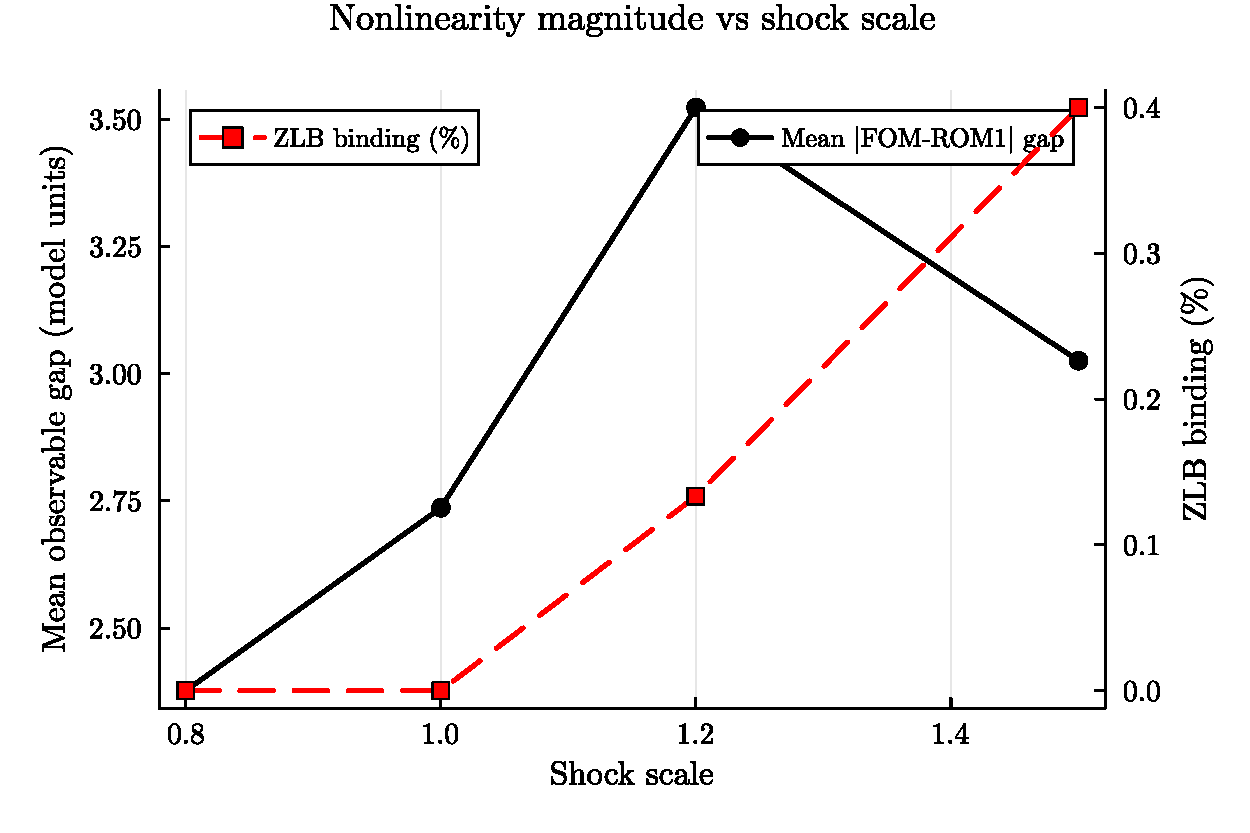
\includegraphics[width=\textwidth]{figures/gap_magnitude_vs_shock_scale.pdf}
\caption{FOM--ROM1 gap magnitude and lower-bound binding diagnostics across the plotted shock-scale grid. The left axis reports the total squared transition-function gap; the right axis reports lower-bound binding frequency and binding-period investment share. Investment/capital remains the largest contributor over the displayed range; at the most extreme scale (1.5$\sigma$), the binding-period share is based on only 3 binding periods.}
\label{fig:gap_magnitude_vs_scale}
\end{figure}

\begin{figure}[htbp]
\centering
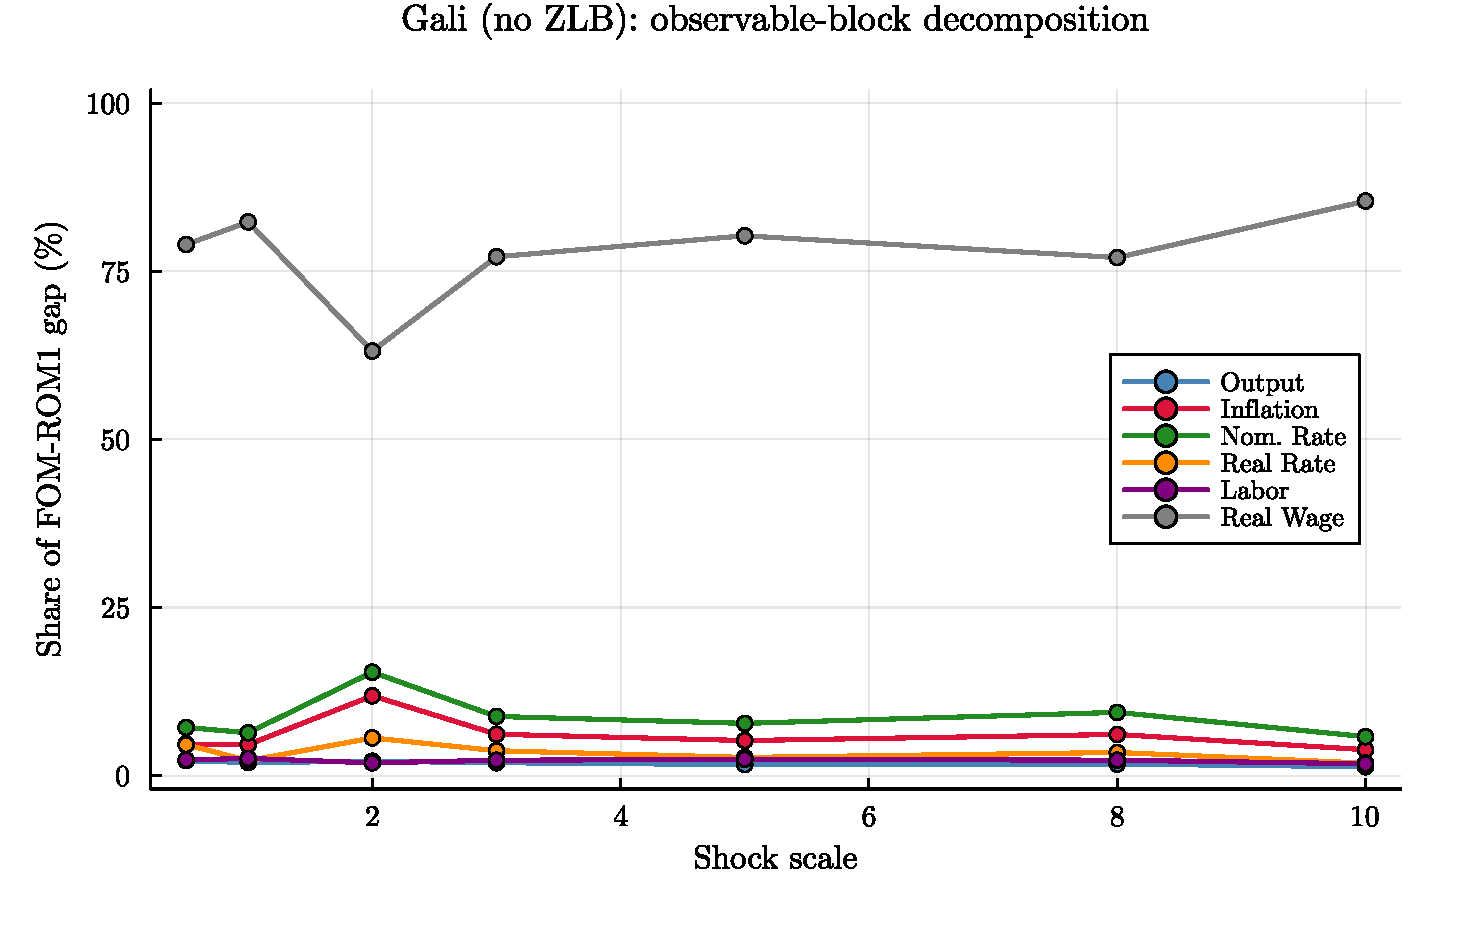
\includegraphics[width=\textwidth]{figures/gali_block_decomposition.pdf}
\caption{FOM--ROM1 gap decomposition in the Gal\'i (2015) model, which shares the ELB and Kimball structure with the HLT model but lacks investment. Shares are percentages of the total squared transition-function gap at each shock scale. The plotted gap is much smaller than in the HLT model at every shock scale, consistent with the investment channel being the main difference between the models.}
\label{fig:gali_block_decomposition}
\end{figure}


\section{Out-of-Sample Forecast Comparison}
\label{app:oos_forecast}

One natural question about the COVID-era results in Section~\ref{subsec:extended_sample} is whether the nonlinear model's better in-sample criterion value translates into better out-of-sample predictive performance---particularly over the COVID window that dominates the in-sample objective gap. This appendix reports a pseudo-out-of-sample exercise: I re-estimate both models on the pre-COVID sample 1959Q1--2019Q4 ($T_{\text{pre}} = 244$ quarters) and compute one-step-ahead conditional-prediction RMSE for each observable over the holdout window 2020Q1--2025Q1 ($T_{\text{fore}} = 21$ quarters).

\paragraph{Design.} I truncate the extended-sample data to 1959Q1--2019Q4 and re-run (i) the linear Kalman-NUTS chain and (ii) the surrogate regime-switching chain on the restricted sample, each warm-started from the corresponding full-sample posterior mean to reduce warmup cost. I use 500 post-warmup NUTS draws for the linear chain and 300 for the surrogate (reduced from the paper's main-text 2{,}000 because warm-starting largely eliminates the adaptation-period requirement; pooled ESS values in the linear chain on 500 draws exceed 120 for all but three parameters). From each pre-COVID chain I then evaluate the 21-period holdout window via one-step-ahead conditional predictions: for each posterior draw $\theta^{(j)}$, I run the Kalman smoother (linear) or inversion filter with surrogate correction (regime-switching) up to $T_{\text{pre}}$ to obtain the final filtered state $\hat{s}_{T_{\text{pre}}}$, then recover holdout shocks period by period when forming $\hat{y}_{t+1|t}$ for $t \in \{T_{\text{pre}}, \ldots, T_{\text{pre}} + T_{\text{fore}} - 1\}$. These are conditional filtering diagnostics, not real-time unconditional forecasts. RMSE is computed per observable as $\text{RMSE}_j = \sqrt{\frac{1}{T_{\text{fore}}}\sum_{t} (y_{t+1,j} - \hat{y}_{t+1|t,j})^2}$.

\paragraph{Results.} Table~\ref{tab:oos_forecast} reports the one-step-ahead conditional-prediction RMSE per observable over three windows: the full OOS period 2020Q1--2025Q1 (21 quarters), the COVID window 2020Q1--2021Q2 (6 quarters), and the post-COVID recovery 2021Q3--2025Q1 (15 quarters). The pattern is informative. During the COVID window the switching surrogate outperforms ROM1 on the four quantity aggregates---output growth (29 percent RMSE reduction), consumption (24 percent), investment (26 percent), and wage growth (8 percent)---and on the aggregate RMSE by 16 percent. These are the observables in which the investment-channel nonlinearity matters most, and the ranking is consistent with the in-sample decomposition in Section~\ref{subsec:nonlinearity_sources}. Over the post-COVID window, the ranking flips: ROM1 delivers smaller RMSE across most observables, reflecting that the regime-switching gate continues to fire through the recovery even as the underlying dynamics return to the linear regime. On the full OOS sample the aggregate RMSE ratio is $1.14$---the switching model's COVID gains are partly offset by its post-COVID over-activation, yielding a narrow overall ROM1 advantage.

\begin{table}[htbp]
\centering
\caption{Out-of-sample one-step-ahead conditional-prediction RMSE: 2020Q1--2025Q1}
\label{tab:oos_forecast}
\small
\begin{tabular}{lcccccccccc}
\toprule
& \multicolumn{3}{c}{Full OOS (21Q)} & \multicolumn{3}{c}{COVID (6Q)} & \multicolumn{3}{c}{Post-COVID (15Q)} \\
\cmidrule(lr){2-4} \cmidrule(lr){5-7} \cmidrule(lr){8-10}
Observable & ROM1 & Switch & Ratio & ROM1 & Switch & Ratio & ROM1 & Switch & Ratio \\
\midrule
$\Delta y$   & 3.61 & 2.61 & 0.72 & 6.66 & 4.74 & 0.71 & 0.71 & 0.74 & 1.04 \\
$\Delta c$   & 3.84 & 2.93 & 0.76 & 7.05 & 5.34 & 0.76 & 0.92 & 0.81 & 0.88 \\
$\Delta i$   & 7.54 & 7.56 & 1.00 & 13.29 & 9.85 & 0.74 & 3.00 & 6.41 & 2.14 \\
Labor        & 1.53 & 5.97 & 3.90 & 2.68 & 6.36 & 2.38 & 0.65 & 5.81 & 9.00 \\
$\pi$        & 0.49 & 1.36 & 2.78 & 0.71 & 1.08 & 1.52 & 0.37 & 1.46 & 3.96 \\
$\Delta w$   & 2.21 & 1.95 & 0.88 & 3.06 & 2.82 & 0.92 & 1.76 & 1.47 & 0.83 \\
$R$          & 0.34 & 2.28 & 6.79 & 0.58 & 2.01 & 3.47 & 0.15 & 2.38 & 15.72 \\
\midrule
Aggregate    & 3.63 & 4.12 & 1.14 & 6.41 & 5.37 & \textbf{0.84} & 1.42 & 3.51 & 2.48 \\
\bottomrule
\end{tabular}
\smallskip
\tablenotes{\textit{Notes}: One-step-ahead conditional-prediction RMSE at the pre-COVID posterior mean. ``ROM1'' uses the Kalman filter with the linear posterior mean from a 500-draw pre-COVID NUTS chain (min ESS $= 141$). ``Switch'' uses the inversion filter with the regime-switching surrogate at the surrogate posterior mean from a 300-draw pre-COVID NUTS chain (min ESS $= 80$), with soft gating calibrated on the pre-COVID sample. Holdout shocks are recovered period by period by the evaluator, so these are conditional filtering diagnostics rather than real-time unconditional forecasts. Ratio below 1 indicates the switching model produces smaller prediction errors. Estimation sample: 1959Q1--2019Q4 ($T_{\text{pre}} = 244$); evaluation sample: 2020Q1--2025Q1 ($T_{\text{fore}} = 21$). Aggregate RMSE is the root of the mean squared error pooled across all 7 observables, normalizing each observable by its in-sample standard deviation to make the aggregation scale-invariant.}
\end{table}

\paragraph{Interpretation.} The COVID-window result---a 16 percent reduction in aggregate RMSE, driven by 24--29 percent reductions on output, consumption, and investment---is a stress-window diagnostic. The nonlinear model is designed to activate during stressed episodes; 2020Q1--2021Q2 is the canonical stressed episode for post-war U.S. data, and the switching model delivers measurable conditional-prediction gains over the linear alternative. For investment growth during COVID, RMSE falls from 13.29 to 9.85, consistent with the equation-block decomposition assigning 69 percent of the nonlinearity to the investment block.

Two caveats apply. First, the post-COVID under-performance appears partly gate-related rather than solely model-fundamental: the gate threshold calibrated on the pre-COVID sample treats 2021Q3--2025Q1 as more stressed than the economy actually is, firing the NN correction in quarters when ROM1 would fit better. Re-calibrating the gate with a post-COVID tail adjustment, or moving to the soft-gate mixture formulation (Section~\ref{app:gate}) across the full holdout, is a natural robustness check. Second, the labor and interest-rate observables show large ratios in both windows; these observables enter the inversion filter's shock-recovery step and are therefore sensitive to the filter architecture, not just to the underlying model solution. I report the disaggregated numbers for transparency; the aggregate and block-level results are the quantitatively meaningful objects.

\paragraph{Quiet-sample diagnostic.} To test whether the same gate/surrogate design damages calm-period performance, I run a bounded quiet-sample pilot: estimate both models through 1994Q4 ($T_{\text{pre}} = 144$), then score one-step-ahead conditional predictions over 1995Q1--2007Q4 (52 quarters). The chains are shorter than the main posterior runs (200 linear draws and 150 surrogate draws, both warm-started from the full-sample posterior means, with zero post-warmup divergences), so this is a failure-mode diagnostic rather than a final forecasting comparison. Table~\ref{tab:oos_forecast_quiet} reports the original-gate results. Under the original gate, the acceptance criterion is not met. The switching surrogate's aggregate RMSE is 2.40 times ROM1 over the full quiet holdout, despite improving output and consumption growth. The degradation is concentrated in labor, inflation, and the policy rate, and the original hard gate is active throughout the quiet holdout.

I then run a fixed-posterior gate-recalibration diagnostic using the same quiet-sample chains. This diagnostic changes only the stored gate policy used by the evaluator; it does not re-estimate the surrogate posterior and should therefore be read as a localization exercise rather than a final forecasting result. Table~\ref{tab:oos_gate_recalibration} shows that the original quiet failure is largely a gate-stickiness problem. A baseline no-padding diagnostic lowers the aggregate ratio to 1.18 and the hard-gate share to 1.9 percent. A stricter q95 threshold with default padding performs best, lowering the aggregate ratio to 1.04, the remaining-window ratio to 1.03, and the hard-gate share to 1.9 percent. This substantially narrows the calm-period failure but does not close it: ROM1 still wins slightly.

Finally, I re-estimate the surrogate chain under the q95 padded gate. The chain has 150 post-warmup draws, zero post-warmup divergences, and posterior-mean objective $-844.95$ on the quiet estimation sample. Table~\ref{tab:oos_q95_reestimated} shows that re-estimation keeps the qualitative lesson from the fixed-posterior diagnostic but weakens the headline number. The full quiet-window aggregate ratio is 1.09, much better than the original-gate ratio of 2.40 but still worse than ROM1. The early quiet window favors the switching surrogate (0.70), while the remaining quiet window favors ROM1 (1.19). I therefore treat quiet-sample performance as an unresolved gate-design risk, not as evidence overturning the in-sample nonlinear posterior result.

\begin{table}[htbp]
\centering
\caption{Quiet-sample one-step-ahead conditional-prediction RMSE: 1995Q1--2007Q4}
\label{tab:oos_forecast_quiet}
\small
\begin{tabular}{lcccccccccc}
\toprule
& \multicolumn{3}{c}{Full OOS (52Q)} & \multicolumn{3}{c}{Early quiet (16Q)} & \multicolumn{3}{c}{Remaining (36Q)} \\
\cmidrule(lr){2-4} \cmidrule(lr){5-7} \cmidrule(lr){8-10}
Observable & ROM1 & Switch & Ratio & ROM1 & Switch & Ratio & ROM1 & Switch & Ratio \\
\midrule
$\Delta y$   & 1.265 & 0.525 & 0.41 & 1.335 & 0.450 & 0.34 & 1.233 & 0.554 & 0.45 \\
$\Delta c$   & 1.866 & 0.463 & 0.25 & 1.793 & 0.370 & 0.21 & 1.897 & 0.498 & 0.26 \\
$\Delta i$   & 1.505 & 4.736 & 3.15 & 1.125 & 5.398 & 4.80 & 1.645 & 4.411 & 2.68 \\
Labor        & 0.476 & 4.470 & 9.38 & 0.585 & 2.473 & 4.23 & 0.420 & 5.113 & 12.19 \\
$\pi$        & 0.166 & 2.084 & 12.53 & 0.155 & 2.199 & 14.17 & 0.171 & 2.030 & 11.88 \\
$\Delta w$   & 0.888 & 0.731 & 0.82 & 0.464 & 0.489 & 1.05 & 1.021 & 0.816 & 0.80 \\
$R$          & 0.239 & 0.955 & 3.99 & 0.248 & 0.450 & 1.82 & 0.236 & 1.108 & 4.70 \\
\midrule
Aggregate    & 1.098 & 2.637 & \textbf{2.40} & 0.993 & 2.416 & 2.43 & 1.142 & 2.730 & 2.39 \\
\bottomrule
\end{tabular}
\smallskip
\tablenotes{\textit{Notes}: One-step-ahead conditional-prediction RMSE at the quiet-sample posterior means. ROM1 uses the Kalman filter with a 200-draw linear NUTS chain. Switch uses the inversion filter with the regime-switching surrogate at the posterior mean from a 150-draw surrogate NUTS chain. Both chains are warm-started from the full-sample posterior means and have zero post-warmup divergences. Holdout shocks are recovered period by period by the evaluator, so these are conditional filtering diagnostics rather than real-time unconditional forecasts. Estimation sample: 1959Q1--1994Q4 ($T_{\text{pre}} = 144$); evaluation sample: 1995Q1--2007Q4. The early quiet window is 1995Q1--1998Q4. Ratio below 1 indicates the switching model produces smaller prediction errors. Hard-gate shares are 100.0 percent in all quiet windows under the original hard gate; soft-gate mean probabilities are unavailable for this gate configuration.}
\end{table}

\begin{table}[htbp]
\centering
\caption{Quiet-sample gate-recalibration diagnostic}
\label{tab:oos_gate_recalibration}
\small
\resizebox{\textwidth}{!}{%
\begin{tabular}{lcccccc}
\toprule
Gate & Threshold & Padding & Full & Early & Remaining & Hard gate \\
\midrule
Base, no pad & Baseline & 0/0/1 & 1.18 & 1.48 & 1.06 & 1.9\% \\
q95, padded & 0.95 & 4/8/4 & \textbf{1.04} & \textbf{1.07} & \textbf{1.03} & 1.9\% \\
q95, no pad & 0.95 & 0/0/1 & 1.19 & 1.48 & 1.08 & 0.0\% \\
q98, no pad & 0.98 & 0/0/1 & 1.20 & 1.50 & 1.09 & 0.0\% \\
\bottomrule
\end{tabular}
}
\smallskip
\tablenotes{\textit{Notes}: Fixed-posterior diagnostic using the quiet-sample chains from Table~\ref{tab:oos_forecast_quiet}. Only the gate calibration and padding rule supplied to the evaluator change. Padding is reported as $k_{\mathrm{pre}}/k_{\mathrm{post}}/\text{min\_len}$. Ratios are aggregate RMSE ratios, with values below 1 favoring the switching surrogate.}
\end{table}

\begin{table}[htbp]
\centering
\caption{Quiet-sample q95 re-estimation diagnostic}
\label{tab:oos_q95_reestimated}
\small
\begin{tabular}{lcccc}
\toprule
Run & Full & Early & Remaining & Hard gate \\
\midrule
Fixed posterior q95 & 1.04 & 1.07 & 1.03 & 1.9\% \\
Re-estimated q95 & 1.09 & 0.70 & 1.19 & 1.9\% \\
\bottomrule
\end{tabular}
\smallskip
\tablenotes{\textit{Notes}: Aggregate RMSE ratios for the q95 padded gate, where values below 1 favor the switching surrogate. The fixed-posterior row holds the original quiet-sample chains fixed and changes only the evaluator gate. The re-estimated row uses a new 150-draw surrogate NUTS chain estimated through 1994Q4 under the q95 padded gate, with zero post-warmup divergences and posterior-mean objective $-844.95$.}
\end{table}


\section{Additional Robustness Checks}
\label{app:robustness_extended}

This appendix presents extended robustness checks and full 18-parameter results.

\begin{table}[htbp]
\centering
\caption{Surrogate Accuracy by Parameter Region}
\label{tab:surrogate_regional_accuracy}
\begin{tabular}{lcccc}
\toprule
Parameter Region & $N_{\text{test}}$ & RRMSE (median) & RRMSE (95th pctl) & Worst Variable \\
\midrule
Core (0-25th pctl) & 1,250 & 0.00062 & 0.00098 & Capital \\
Mid-Low (25-50th) & 1,250 & 0.00078 & 0.00124 & Inflation \\
Mid-High (50-75th) & 1,250 & 0.00091 & 0.00156 & Output gap \\
Tail (75-100th) & 1,250 & 0.00135 & 0.00231 & Real rate \\
\bottomrule
\end{tabular}
\smallskip
\tablenotes{\textit{Notes}: Distance measured as Mahalanobis norm from prior mean. The median RRMSE is below 0.002 in every region; the tail-region 95th percentile exceeds 0.002, so far-tail accuracy remains a caveat.}
\end{table}

\subsection{Excluded Validation Tables}

Seed-sensitivity, prior-sensitivity, simplified 18-parameter validation, and sample-length recovery tables are excluded because the replication package does not contain documented runs supporting those numerical claims. Appendix~\ref{sec:validation_design} tracks the passing hard-ELB Gal\'i package audit, the reduced HLT direct-SEP bridge, and the remaining full multi-period direct-SEP HMC scaling targets.

\subsection{Surrogate Architecture Comparison}

The architecture-comparison table is also excluded because its posterior-mode errors came from the same unsupported three-parameter recovery exercise. The paper uses the architecture documented in the training materials and reports only held-out accuracy and posterior consequences with matching replication support.

\subsection{ZLB-Binding Surrogate Performance}

\begin{figure}[htbp]
\centering
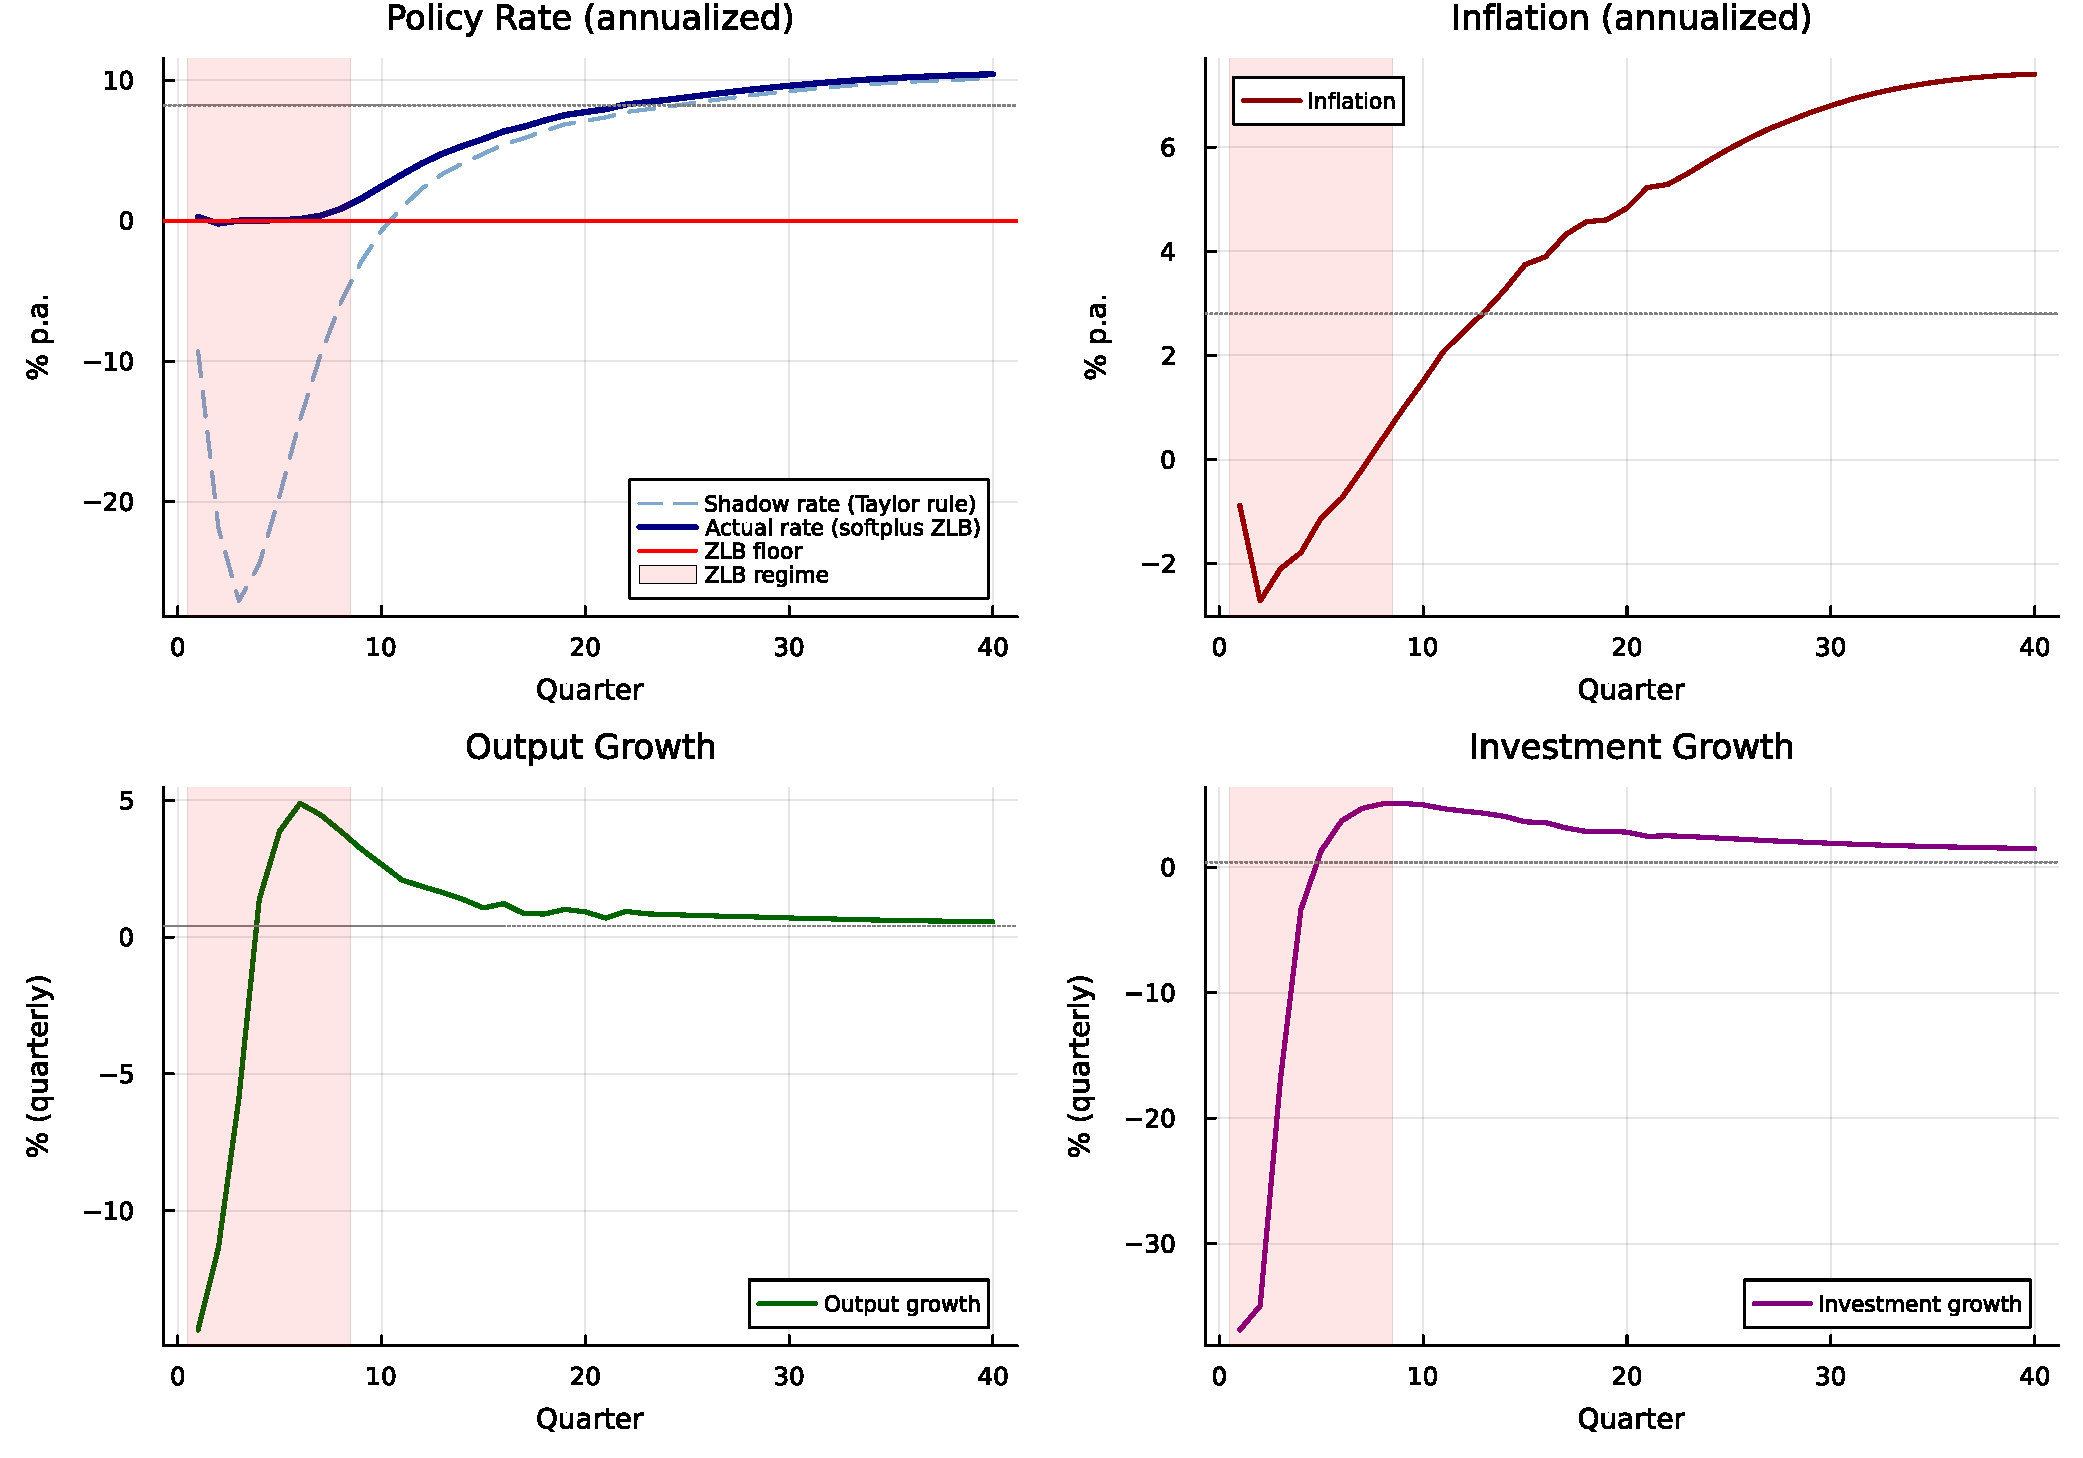
\includegraphics[width=0.88\textwidth]{figures/fig_zlb_binding_simulation.pdf}
\caption{ZLB-binding simulation using the SEP nonlinear solver with the softplus formulation ($\kappa_s = 100$). Top-left: shadow rate (dashed) versus actual rate (solid); red shading marks quarters where the actual annualized rate is below 1\%. Top-right: annualized inflation. Bottom-left: output growth. Bottom-right: investment growth. Shocks: $\varepsilon^b = (-2, -1, -0.5)\sigma$ and $\varepsilon^{qs} = (-1, -0.5)\sigma$ in the first three quarters. Gray dotted lines mark steady-state values.}
\label{fig:zlb_binding_simulation}
\end{figure}

\begin{figure}[htbp]
\centering
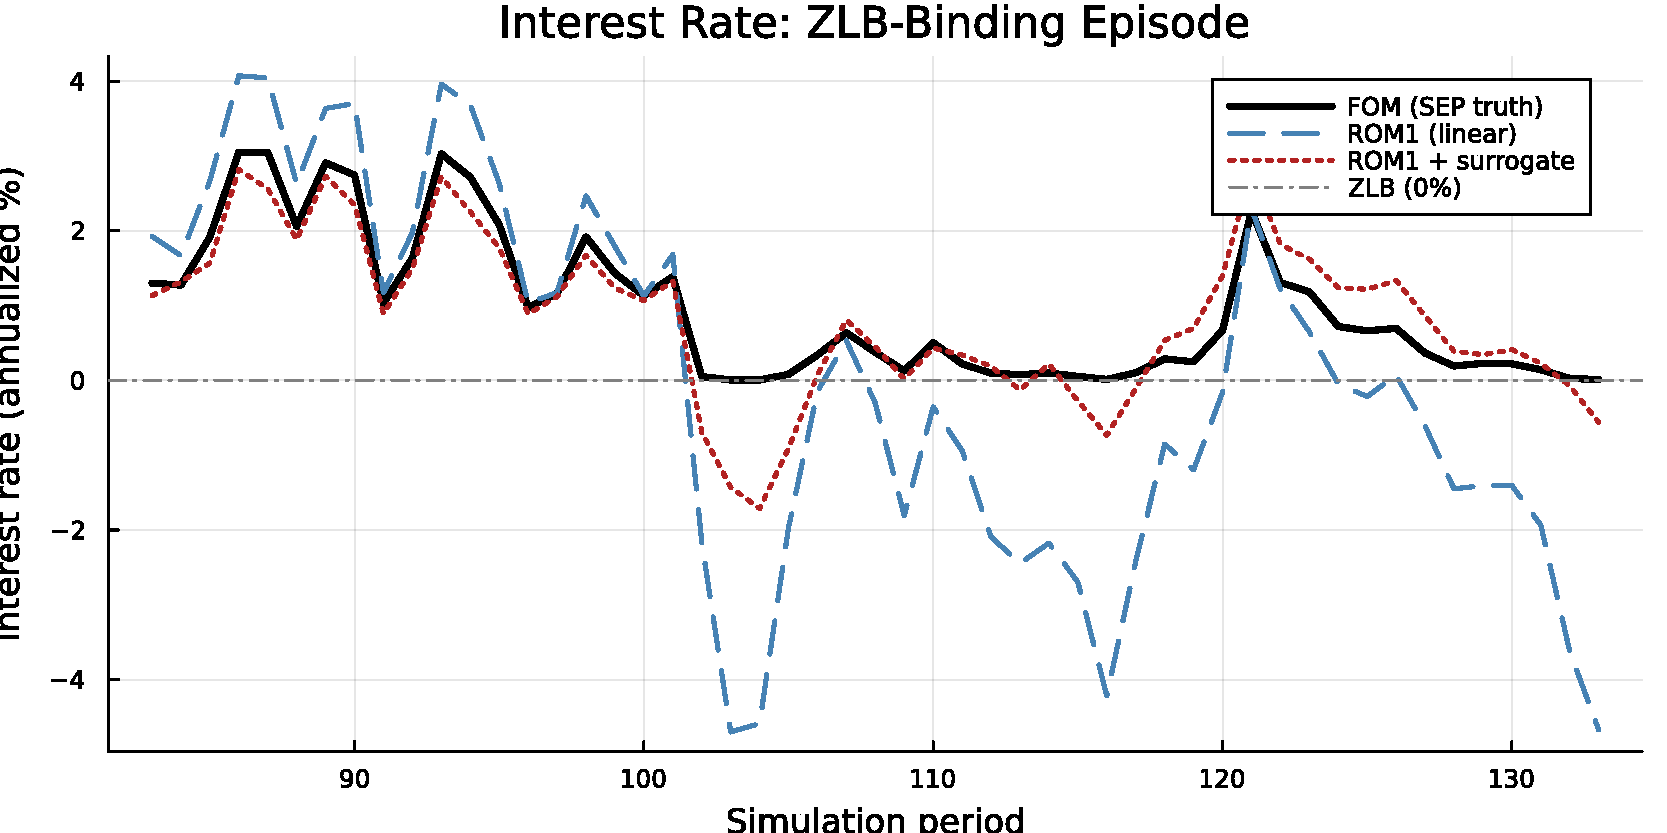
\includegraphics[width=0.95\textwidth]{figures/zlb_correction_robs_closeup.pdf}
\caption{Interest rate during a ZLB-binding episode. Black solid: FOM (SEP). Blue dashed: ROM1 (predicts negative rates). Red dotted: ROM1 + surrogate correction. Gray: ZLB floor. Shock scale 0.4, SW07-HLT model.}
\label{fig:zlb_correction_robs}
\end{figure}

\begin{figure}[htbp]
\centering
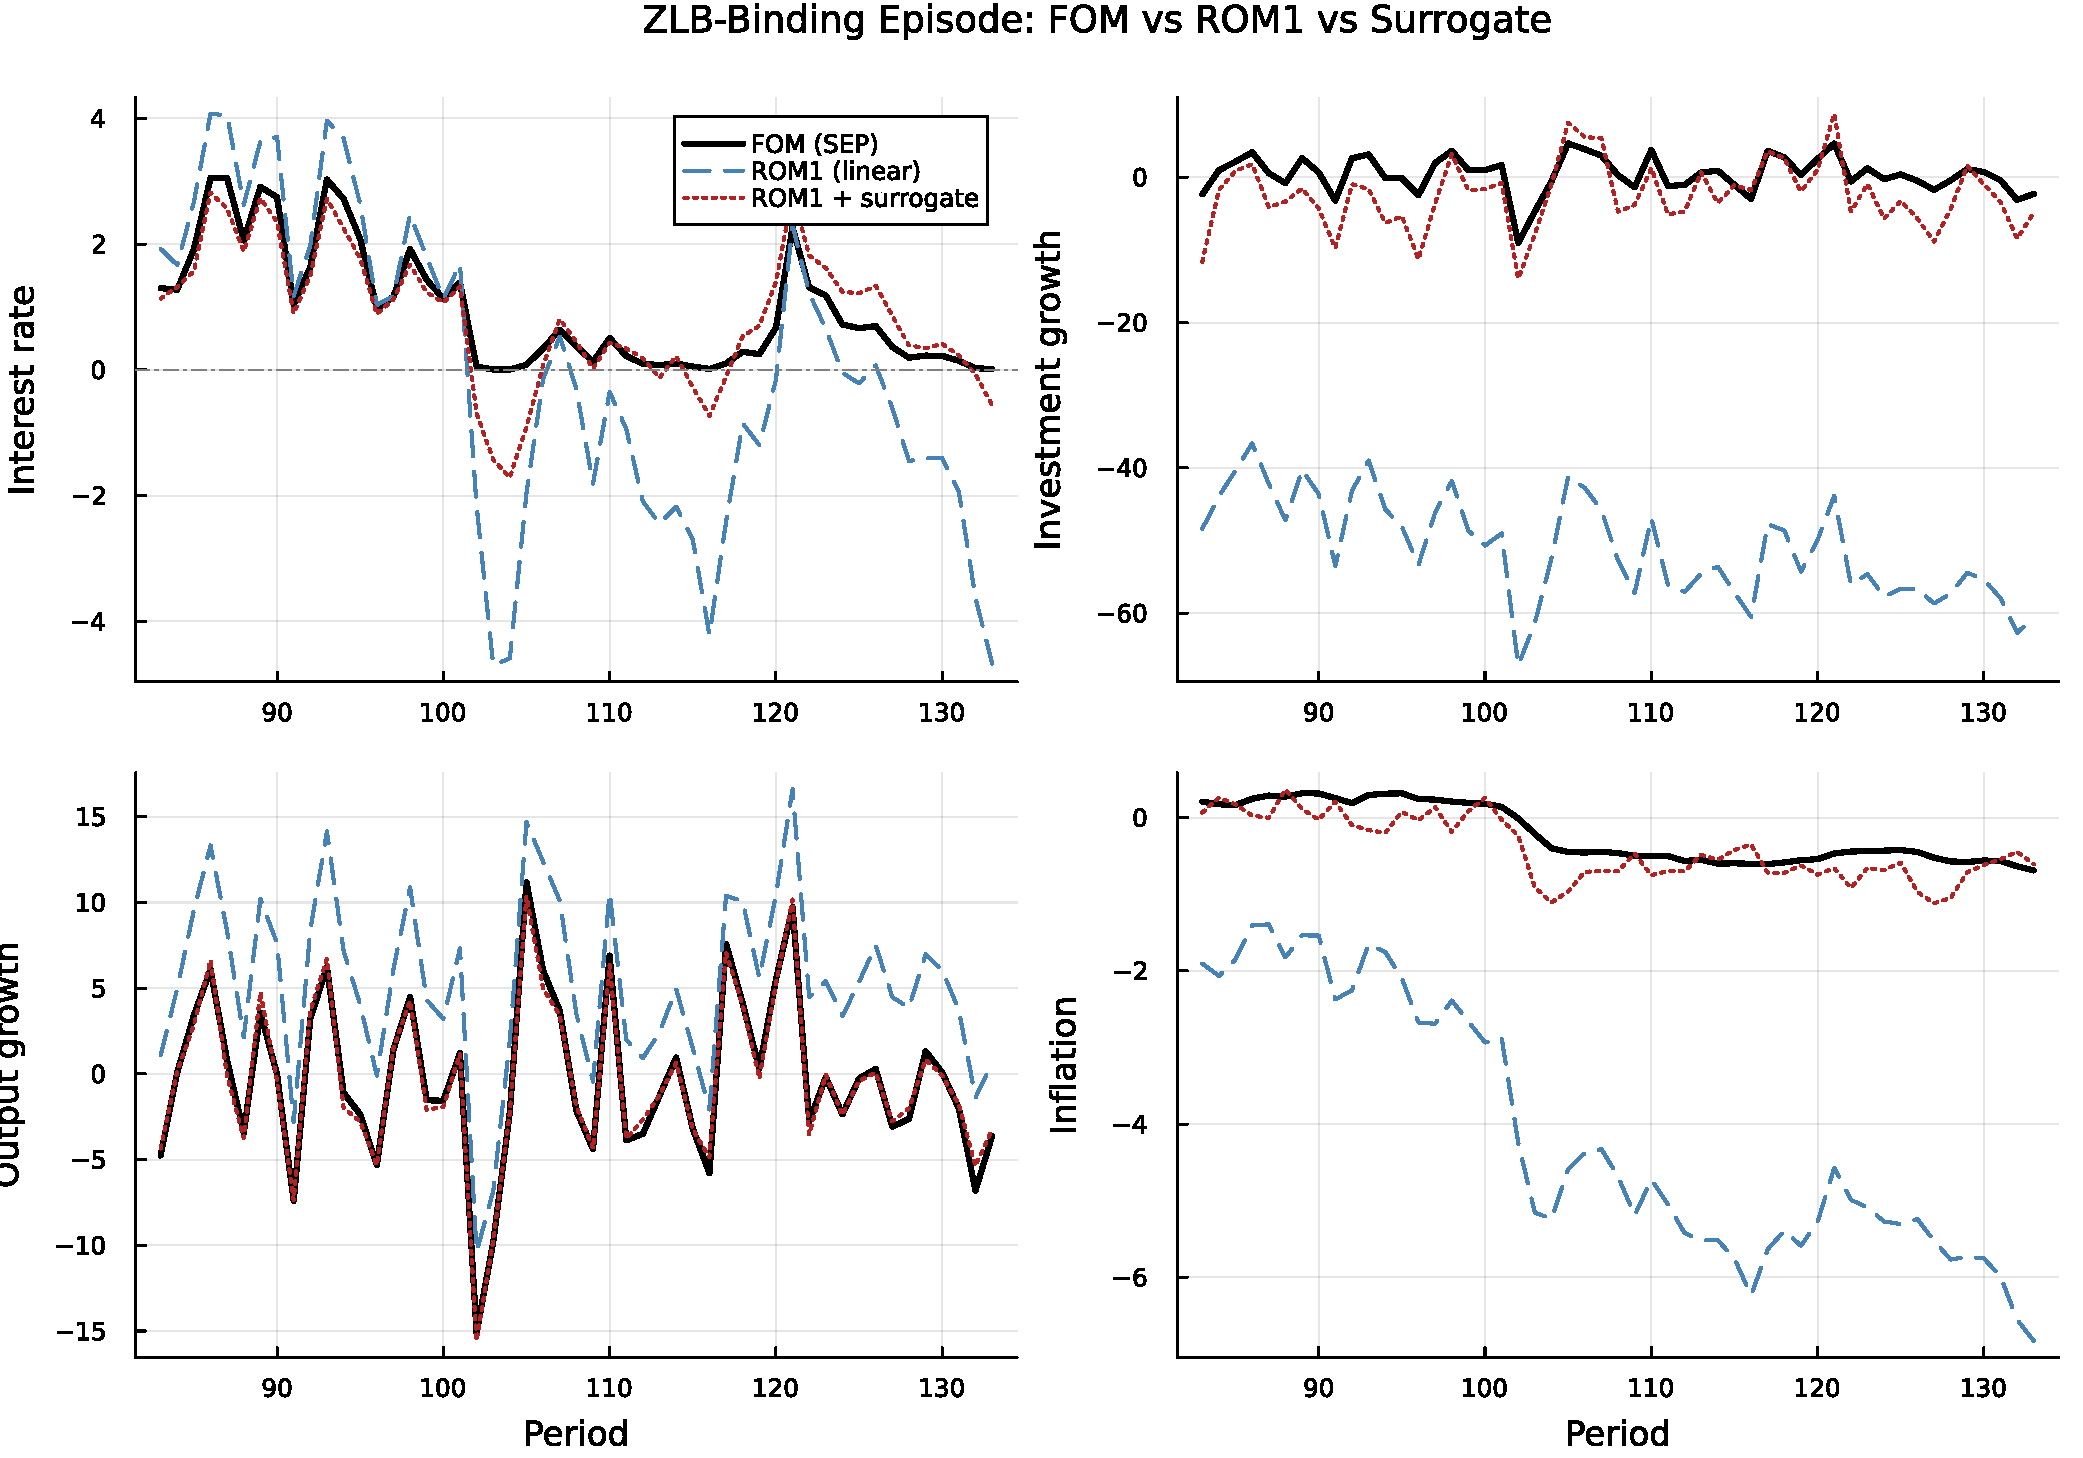
\includegraphics[width=0.95\textwidth]{figures/zlb_correction_timeseries_4panel.pdf}
\caption{Four-observable comparison during a ZLB-binding episode. ROM1 + surrogate (red dotted) tracks the SEP benchmark (black solid); ROM1 alone (blue dashed) diverges. Investment growth shows the largest corrections, consistent with the investment-dominance finding.}
\label{fig:zlb_correction_4panel}
\end{figure}


\section{Linear Baseline: Comparison with Farkas and Tat\'ar (2020)}
\label{app:hlt_vs_ft}
\label{app:ft_comparison}

The linear HMC baseline in Table~\ref{tab:18param_posterior} uses the Holden--Lind\'e--Trabandt (HLT) reparameterization of the \citet{smets2007shocks} model, which differs from the original specification in ways that affect posterior comparison with earlier work. This appendix documents these differences, compares the 18-parameter HMC posterior to the results in \citet{farkas2020bayesian}, and reports a sensitivity analysis restoring the moving-average (MA) markup structure.

\subsection{Model Differences}

The HLT specification departs from the base \citet{smets2007shocks} model in three ways relevant to posterior comparison:

The markup shock dynamics differ most consequentially. The original SW07 model specifies price and wage markup shocks as ARMA(1,1):
\[
s_t^{\pi} = \rho_\pi s_{t-1}^{\pi} + \varepsilon_t - \mu_p \varepsilon_{t-1}, \qquad
s_t^{w} = \rho_w s_{t-1}^{w} + \eta_t - \mu_w \eta_{t-1}.
\]
\citet{farkas2020bayesian} estimate $\mu_p = 0.80$ and $\mu_w = 0.89$ and show that this markup ARMA block contributes to a flat posterior target in the full Smets--Wouters specification. The HLT baseline fixes $\mu_p = \mu_w = 0$, eliminating the MA component entirely. This transfers the burden of generating inflation and wage persistence from the MA terms onto other parameters---principally indexation ($\iota_p$) and the AR coefficients ($\rho_\pi$, $\rho_w$).

The SCALE1 reparameterization adds another comparison issue. Shock innovations in HLT enter as $z_{\varepsilon}/100 \times \textit{SCALE1}_\varepsilon$, where the scaling factor is the inverse Phillips-curve slope at the parameter vector. This makes volatility parameters scale-independent of Calvo and Kimball parameters but makes the $z$ values not directly comparable to the raw $\sigma$ parameters in the standard specification.

Finally, the HLT model includes a Kimball demand curvature parameter $\varepsilon_p$ (estimated at 78 in Table~\ref{tab:18param_posterior}) that the original SW07 model does not have. The Kimball term flattens the Phillips curve slope by a factor of $1/[(\varepsilon_p - 1) S''(1) + 1]$, requiring higher Calvo stickiness to match observed inflation dynamics.

\subsection{Comparison with Farkas and Tat\'ar (2020)}

Table~\ref{tab:ft_comparison} compares the HLT baseline posterior to the HMC results from \citet{farkas2020bayesian}, who estimate the full SW07 specification (36 parameters) on the 1960Q1--2004Q4 sample using NUTS via Stan with 1,000 draws.

\begin{table}[htbp]
\centering
\caption{Posterior Comparison: HLT Baseline vs.\ Farkas--Tat\'ar (2020)}
\label{tab:ft_comparison}
\begin{tabular}{llccc}
\toprule
Parameter & Description & FT (2020) & HLT $\mu=0$ & HLT $\mu=\text{SW07}$ \\
\midrule
\multicolumn{5}{l}{\textit{Shock Persistence}} \\
$\rho_a$ & TFP & 0.98 & 0.986 & 0.987 \\
$\rho_b$ & Risk premium & 0.27 & 0.702 & 0.793 \\
$\rho_g$ & Government & 0.97 & 0.986 & 0.986 \\
$\rho_{qs}$ & Investment & 0.69 & 0.771 & 0.750 \\
$\rho_\pi$ & Price markup & 0.96 & 0.026 & 0.091 \\
$\rho_w$ & Wage markup & 0.97 & 0.391 & 0.751 \\
$\rho_{ms}$ & Monetary & 0.17 & 0.162 & 0.169 \\
\midrule
\multicolumn{5}{l}{\textit{Shock Volatilities}} \\
$\sigma_a$ & TFP & 0.48 & 0.505 & 0.505 \\
$\sigma_b$ & Risk premium & 0.24 & 0.142 & 0.106 \\
$\sigma_g$ & Government & 0.52 & 0.507 & 0.507 \\
$\sigma_{qs}$ & Investment & 0.46 & 0.363 & 0.376 \\
$\sigma_\pi$ & Price markup & 0.13 & 0.135 & 0.162 \\
$\sigma_w$ & Wage markup & 0.25 & 0.196 & 0.335 \\
$\sigma_{ms}$ & Monetary & 0.24 & 0.240 & 0.239 \\
\midrule
\multicolumn{5}{l}{\textit{Structural Parameters}} \\
$\xi_p$ & Calvo prices & 0.64 & 0.924 & 0.937 \\
$\iota_p$ & Price indexation & 0.24 & 0.925 & 0.979 \\
$\varepsilon_p$ & Kimball curvature & --- & 77.9 & 81.5 \\
$\xi_w$ & Calvo wages & 0.75 & 0.943 & 0.944 \\
\midrule
$\mu_p$ & Price MA & 0.80 & 0 (fixed) & 0.80 (fixed) \\
$\mu_w$ & Wage MA & 0.89 & 0 (fixed) & 0.89 (fixed) \\
\midrule
\multicolumn{2}{l}{Log-likelihood} & --- & $-1{,}027$ & $-993$ \\
\multicolumn{2}{l}{Draws / min ESS} & 1000 / 287 & 1000 / 501 & 1000 / 660 \\
\multicolumn{2}{l}{Divergences} & 0 & 0 & 0 \\
\bottomrule
\end{tabular}
\smallskip
\tablenotes{\textit{Notes}: ``FT (2020)'' reports posterior means from Table~4--5 of \citet{farkas2020bayesian}, who estimate the full SW07 model (36 parameters) on 1960Q1--2004Q4 data using NUTS via Stan. ``HLT $\mu=0$'' is the baseline from Table~\ref{tab:18param_posterior} (18 parameters, HLT reparameterization, $\mu_p = \mu_w = 0$). ``HLT $\mu=\text{SW07}$'' restores the MA coefficients at the \citet{farkas2020bayesian} posterior values ($\mu_p = 0.80$, $\mu_w = 0.89$) while keeping all other settings identical. Both HLT columns use the same sample (1959Q1--2004Q4, $T=184$), priors, and NUTS configuration. FT volatility parameters are raw $\sigma$; HLT volatilities are $z/100 \times \text{SCALE1}$ and therefore not directly comparable in magnitude. FT does not report log-likelihood or include Kimball curvature.}
\end{table}

\subsection{Discussion}

The comparison reveals which discrepancies arise from the MA specification versus deeper structural differences.

\paragraph{Parameters that match across compared specifications.} Technology persistence ($\rho_a \approx 0.98$), government spending persistence ($\rho_g \approx 0.97$--0.99), monetary policy persistence ($\rho_{ms} \approx 0.17$), and the shock volatilities for technology, government, and monetary policy ($\sigma_a$, $\sigma_g$, $\sigma_{ms}$) are stable across the compared HLT specifications. These parameters appear better identified than the markup block in this comparison.

\paragraph{Parameters sensitive to the MA terms.} Restoring $\mu_p = 0.80$ and $\mu_w = 0.89$ produces large shifts in wage markup persistence ($\rho_w$: $0.39 \to 0.75$, toward the FT value of 0.97) and improves the log-likelihood by 34 nats ($-1{,}027 \to -993$). The MA terms provide a ``first-period kick'' in the markup shocks that the pure AR specification must approximate through higher $\rho_w$ or, when $\rho_w$ is constrained, through indexation and Calvo stickiness. This is not a cosmetic specification choice: \citet{farkas2020bayesian} identify the ARMA markup block as a source of posterior flatness in the full SW07 target. Price markup persistence ($\rho_\pi$) rises modestly ($0.03 \to 0.09$) but remains far below the FT value of 0.96; the SCALE1 reparameterization and Kimball curvature prevent convergence to the standard SW07 posterior for this parameter.

\paragraph{Parameters driven by Kimball curvature.} Calvo price and wage stickiness ($\xi_p$, $\xi_w$) and price indexation ($\iota_p$) are substantially higher in both HLT specifications than in FT. This is a consequence of the Kimball aggregator ($\varepsilon_p \approx 80$), which flattens the Phillips curve slope and requires higher nominal rigidity to match observed inflation dynamics. These parameters are structurally incomparable without accounting for the Kimball term.

\paragraph{Remaining discrepancies.} Risk premium persistence ($\rho_b$) is higher in both HLT runs (0.70--0.79) than in FT (0.27). This likely reflects the 18 fixed structural parameters---habit formation, investment adjustment costs, risk aversion---whose estimation in FT interacts with the risk premium process. Similarly, the risk premium volatility $\sigma_b$ is lower in the HLT specification (0.11--0.14 vs.\ FT's 0.24), plausibly because the SCALE1 reparameterization rescales the effective shock size.

The 34-nat log-likelihood improvement from restoring the MA terms materially improves in-sample fit and changes the posterior geometry. For the nonlinear estimation in the main text, I retain the HLT default ($\mu_p = \mu_w = 0$) to maintain consistency with the surrogate training data, noting that future work should explore estimating the MA coefficients jointly with the structural parameters.


\clearpage

\fi
\end{document}
